% Options for packages loaded elsewhere
\PassOptionsToPackage{unicode}{hyperref}
\PassOptionsToPackage{hyphens}{url}
%
\documentclass[
  12pt,
  openany]{book}
\usepackage{lmodern}
\usepackage{setspace}
\usepackage{amsmath}
\usepackage{ifxetex,ifluatex}
\ifnum 0\ifxetex 1\fi\ifluatex 1\fi=0 % if pdftex
  \usepackage[T1]{fontenc}
  \usepackage[utf8]{inputenc}
  \usepackage{textcomp} % provide euro and other symbols
  \usepackage{amssymb}
\else % if luatex or xetex
  \usepackage{unicode-math}
  \defaultfontfeatures{Scale=MatchLowercase}
  \defaultfontfeatures[\rmfamily]{Ligatures=TeX,Scale=1}
\fi
% Use upquote if available, for straight quotes in verbatim environments
\IfFileExists{upquote.sty}{\usepackage{upquote}}{}
\IfFileExists{microtype.sty}{% use microtype if available
  \usepackage[]{microtype}
  \UseMicrotypeSet[protrusion]{basicmath} % disable protrusion for tt fonts
}{}
\makeatletter
\@ifundefined{KOMAClassName}{% if non-KOMA class
  \IfFileExists{parskip.sty}{%
    \usepackage{parskip}
  }{% else
    \setlength{\parindent}{0pt}
    \setlength{\parskip}{6pt plus 2pt minus 1pt}}
}{% if KOMA class
  \KOMAoptions{parskip=half}}
\makeatother
\usepackage{xcolor}
\IfFileExists{xurl.sty}{\usepackage{xurl}}{} % add URL line breaks if available
\IfFileExists{bookmark.sty}{\usepackage{bookmark}}{\usepackage{hyperref}}
\hypersetup{
  hidelinks,
  pdfcreator={LaTeX via pandoc}}
\urlstyle{same} % disable monospaced font for URLs
\usepackage[left=4cm, right=3cm, top=3cm, bottom=3cm]{geometry}
\usepackage{longtable,booktabs}
\usepackage{calc} % for calculating minipage widths
% Correct order of tables after \paragraph or \subparagraph
\usepackage{etoolbox}
\makeatletter
\patchcmd\longtable{\par}{\if@noskipsec\mbox{}\fi\par}{}{}
\makeatother
% Allow footnotes in longtable head/foot
\IfFileExists{footnotehyper.sty}{\usepackage{footnotehyper}}{\usepackage{footnote}}
\makesavenoteenv{longtable}
\usepackage{graphicx}
\makeatletter
\def\maxwidth{\ifdim\Gin@nat@width>\linewidth\linewidth\else\Gin@nat@width\fi}
\def\maxheight{\ifdim\Gin@nat@height>\textheight\textheight\else\Gin@nat@height\fi}
\makeatother
% Scale images if necessary, so that they will not overflow the page
% margins by default, and it is still possible to overwrite the defaults
% using explicit options in \includegraphics[width, height, ...]{}
\setkeys{Gin}{width=\maxwidth,height=\maxheight,keepaspectratio}
% Set default figure placement to htbp
\makeatletter
\def\fps@figure{htbp}
\makeatother
\setlength{\emergencystretch}{3em} % prevent overfull lines
\providecommand{\tightlist}{%
  \setlength{\itemsep}{0pt}\setlength{\parskip}{0pt}}
\setcounter{secnumdepth}{4}
\PassOptionsToPackage{cmyk}{xcolor}
\usepackage[none]{hyphenat}
\usepackage[cmyk]{xcolor} % Recommended by US-AB
\usepackage{lmodern} % Recommended by US-AB
\usepackage{fancyhdr}
\usepackage{etoolbox}
\patchcmd{\chapter}{\thispagestyle{plain}}{\thispagestyle{fancy}}{}{} % Removes plain pagestyle from chapter headings (otherwise, page numbers are centered)
\AtBeginDocument{\addtocontents{toc}{\protect\thispagestyle{empty}}} 
\pagestyle{empty} % This makes ToC without header/footer
\usepackage[skip=15pt]{caption} % This should increase space below captions (not tested)
\raggedbottom
\usepackage[noindentafter]{titlesec}
\usepackage{titlesec}
\titleformat{\chapter}{\normalfont\bfseries}{\thechapter.}{15pt}{}\titlespacing*{\chapter}{0pt}{-50pt}{0pt}
\titleformat{\section}{\normalfont\bfseries}{\thesection.}{1em}{}\titlespacing*{\section}{0pt}{0pt}{0pt}
\titleformat{\subsection}[runin]{\normalfont\bfseries}{\thesubsection.}{1em}{}
\titleformat{\subsubsection}[runin]{\normalfont\bfseries}{\thesubsubsection.}{1em}{}
\titleformat{\paragraph}[runin]{\normalfont\bfseries}{\theparagraph.}{1em}{}

\usepackage{CJKutf8} % For Mandarin in Acknowledgments

% For guiding quote in beginning of intro:
\makeatletter
% \renewcommand{\@chapapp}{}% Not necessary...
\newenvironment{chapquote}[2][2em]
  {\setlength{\@tempdima}{#1}%
   \def\chapquote@author{#2}%
   \parshape 1 \@tempdima \dimexpr\textwidth-2\@tempdima\relax%
   \itshape}
  {\par\normalfont\hfill--\ \chapquote@author\hspace*{\@tempdima}\par\bigskip}
\makeatother
\usepackage{placeins}
\usepackage{titlesec}
\usepackage{wrapfig}
\usepackage{caption}
\captionsetup[figure]{font=scriptsize}
\usepackage{float}
\usepackage{subcaption}
\usepackage{booktabs}
\usepackage{longtable}
\usepackage{array}
\usepackage{multirow}
\usepackage{wrapfig}
\usepackage{float}
\usepackage{colortbl}
\usepackage{pdflscape}
\usepackage{tabu}
\usepackage{threeparttable}
\usepackage{threeparttablex}
\usepackage[normalem]{ulem}
\usepackage{makecell}
\usepackage{xcolor}
\ifluatex
  \usepackage{selnolig}  % disable illegal ligatures
\fi
\newlength{\cslhangindent}
\setlength{\cslhangindent}{1.5em}
\newlength{\csllabelwidth}
\setlength{\csllabelwidth}{3em}
\newenvironment{CSLReferences}[2] % #1 hanging-ident, #2 entry spacing
 {% don't indent paragraphs
  \setlength{\parindent}{0pt}
  % turn on hanging indent if param 1 is 1
  \ifodd #1 \everypar{\setlength{\hangindent}{\cslhangindent}}\ignorespaces\fi
  % set entry spacing
  \ifnum #2 > 0
  \setlength{\parskip}{#2\baselineskip}
  \fi
 }%
 {}
\usepackage{calc}
\newcommand{\CSLBlock}[1]{#1\hfill\break}
\newcommand{\CSLLeftMargin}[1]{\parbox[t]{\csllabelwidth}{#1}}
\newcommand{\CSLRightInline}[1]{\parbox[t]{\linewidth - \csllabelwidth}{#1}\break}
\newcommand{\CSLIndent}[1]{\hspace{\cslhangindent}#1}

\author{}
\date{\vspace{-2.5em}}

\begin{document}

{
\setcounter{tocdepth}{4}
\tableofcontents
}
\setstretch{1.25}
\cleardoublepage
\pagenumbering{gobble}
\pagestyle{fancy}
\fancyhf{}
\renewcommand{\headrulewidth}{0pt}
\fancyfoot[LE,RO]{\thepage}
\renewcommand{\floatpagefraction}{.9}

\setcounter{page}{11}

\hypertarget{abbreviations}{%
\chapter*{Abbreviations}\label{abbreviations}}
\addcontentsline{toc}{chapter}{Abbreviations}

\begin{longtable}{ll}
\toprule
Abbreviation & Term\\
\midrule
\endfirsthead
\multicolumn{2}{@{}l}{\textit{(continued)}}\\
\toprule
Abbreviation & Term\\
\midrule
\endhead

\endfoot
\bottomrule
\endlastfoot
3' & 3 prime\\
4E-BP & 4E binding protein\\
mcm\textasciicircum{}5s\textasciicircum{}2U & 5-methoxycarbonyl-methyl-2-thiouridine\\
5' & 5 prime\\
m7g & 7-methyl-guanylate\\
\addlinespace
ATF4 & Activating transcription factor 4\\
AMP & Adenosine-mono-phosphate\\
AMPK & Adenosine-mono-phosphate
kinase\\
ATP & Adenosine-tri-phosphate\\
A-site & Aminoacyl-site\\
\addlinespace
aa-tRNA & Aminoacyl-tRNA\\
APV & Analysis of partial varaince\\
ABCE1 & ATP binding cassette protein\\
ARE & AU-rich element\\
ChIP & Chromatin immunoprecipitation\\
\addlinespace
cdsORF & Coding open reading frame\\
CDS & Coding sequence\\
CR-31 & CR-1-31-B\\
CHX & Cyclohexamide\\
CPE & Cytoplasmic polyadenylation\\
\addlinespace
CPEB & Cytoplasmic polyadenylation element binding protein\\
CTU1/2 & Cytosolic thiourdylase 1/2\\
DNA & Deoxyribonucleic acid\\
REDD1 & Development and
DNA damage response 1\\
GADD34 & DNA-inducible gene 34\\
\addlinespace
dsRNA & Double-stranded RNA\\
ELP3 & Elongator acetyltransferase complex subunit 3\\
ER & Endoplasmatic reticulum\\
ERalpha & Estrogen receptor alpha\\
eEF & Eukaryotic elongation factor\\
\addlinespace
eIF & Eukaryotic initiation facotr\\
eRF & Eukaryotic release factor\\
E-site & Exit-site\\
GC/MS & Gas chromatography
mass spectrometry\\
GCN2 & General control nonderepressible 2\\
\addlinespace
GLM & Generalised linear model\\
GDP & Guanosine-di-phosphate\\
GTP & Guanosine-tri-phosphate\\
HRI & Heme regulation eIF2alpha kinase\\
HuR & Human antigen R\\
\addlinespace
HIF-1 & Hypoxia inducible factor 1\\
IGF & Insulin-like growth factor 1\\
IGF1R & Insulin-like growth factor receptor\\
IR & Insulin receptor\\
ISR & Integrated stress response\\
\addlinespace
IRES & Internal ribosome entry site\\
LARP1 & La ribonucleoprotein domain family member 1\\
mTOR & Mammalian/mechatistic target of rapamycin\\
mRNP & Messenger ribonucleoprotein particle\\
mRNA & Messenger RNA\\
\addlinespace
met-tRNAi & Methionyl-initiatior transfer RNA\\
ALKBH8 & Methyltrasnferase TRM9-like domain of alkylation repair homolog 8\\
miRNA & microRNA\\
MAPK & Mitogen-activated protein
kinase\\
NB & Negative binomial\\
\addlinespace
Gld2 & Non-canonical poly(A) polymerase\\
ncRNA & Non-coding RNA\\
ODC1 & Ornithine decarboxylase\\
PDAC & Pancreatic ductal adenocarcinoma\\
P-site & Peptidyl-site\\
\addlinespace
PTEN & Phosphatase and tensin homologue\\
PIP3 & Phosphatidylinositol-3,4,5-trisphosphate\\
PIP2 & Phosphatidylinositol-4,5-bisphosphate\\
PI3K & Phosphoinositide-3-kinase\\
PDK1 & Phosphoinositide-dependent kinase 1\\
\addlinespace
PABP & Poly (A) binding protein\\
PARN & Poly(A) deadynelase\\
PIC & Pre-initiation complex\\
PDCD4 & Programmed cell death protein 4\\
AKT & Protein kinase A\\
\addlinespace
PKR & Protein Kinase R\\
PERK & Protein kinase R-like endoplasmatic reticulum kinase\\
RVM & Random variance model\\
Rheb & Ras homologue enriched in brain\\
ROC & Receiver operating characteristics\\
\addlinespace
RT-qPCR & Reverse transcription quantitative polymerase chain
reaction\\
RNA & Ribonucleic acid\\
rpS6 & Ribosomal protein S6\\
S6K & Ribosomal protein S6 kinases\\
rRNA & Ribosomal RNA\\
\addlinespace
RPF & Ribosome protected fragment\\
RBP & RNA binding protein\\
LKB1 & Serine/threonine kinase 11\\
siRNA & silence RNA\\
sgRNA & Single guide RNA\\
\addlinespace
TOP & Terminal oligopyrimidine\\
TC & Ternary complex\\
tRNA & Transfer RNA\\
TE & Translation efficiency\\
TSC & Tuberous sclerosis complex\\
\addlinespace
UTR & Untranslated region\\
uORF & Upstream open reading frame\\
URM & Urmylation\\
VEGF & Vascular endothelial growth factor\\*
\end{longtable}
\clearpage
\pagenumbering{arabic}

\setcounter{page}{1}

\chapter{Introduction}
\section{Gene expression}
\subsection{The central dogma of gene expression}
  \begin{wrapfigure}{r}{.6\textwidth}
  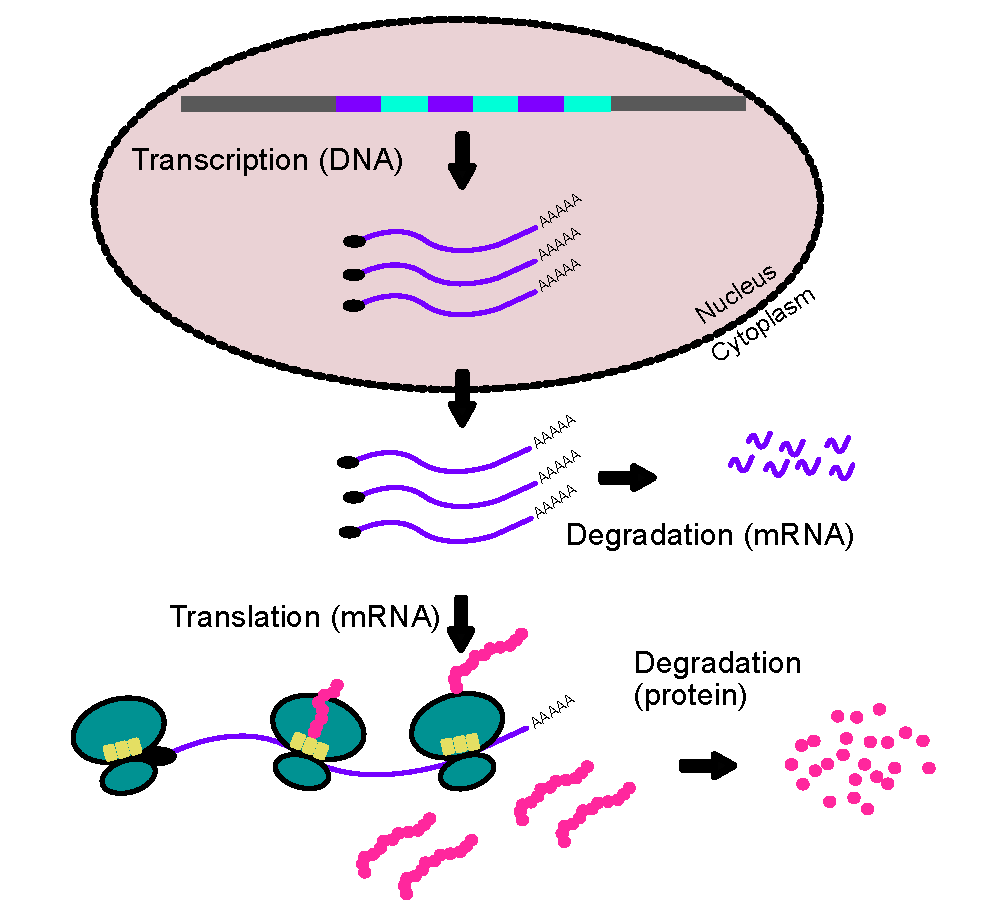
\includegraphics{./figures/geneExprPath_2.pdf}
  \caption{The gene expression pathway - DNA is transcribed into RNA. RNAs are processed into mRNAs that consist of a 5' cap, exons and a poly(A) tail. mRNAs can be transported out of the cellular nucleus into the cytoplasm where they can be degraded, stored, or translated into proteins depending on cellular demands. Synthesised proteins can be degraded by proteosomes. Coloured boxes in the DNA refer to introns (teal) and exons (purple). Introns are non-coding parts of the genome, whereas exons encoding regions. mRNAs are depicted as purple lines, i.e. a series of exons, with an AAAAA extension and an oval shape at its start. Proteins are depicted as a series of pink balls.  \label{fig:geneExprPath}}
\end{wrapfigure}

In eukaryotic cells, genetic code is stored as deoxyribonucleic acid (DNA) molecules in the nucleus. Transcription is the process whereby temporary copies of the DNA are generated and occurs in the nucleus. These copies are called ribonucleic acid (RNA). RNAs undergo processing by which multiple different variants coming from the same gene are produced. A subset of protein-encoding processed RNAs is the so called messenger RNA (mRNA). mRNAs are transported from the nucleus into the cytoplasm where they can be stored, degraded, or translated into proteins. Proteins themselves can also be degraded (\emph{see figure \ref{fig:geneExprPath}}). This flow of genetic information into expressed proteins is commonly referred to as the central dogma in molecular biology (F. Crick, 1970).
\clearpage

\subsection{Contribution to gene expression}

Proteins are the last product of the gene expression pathway and carry out the vast majority of all cellular functions. While it is apparent that modulation of protein levels will offer information on the changes in gene expression, it cannot completely answer the question as to why the protein levels change. In a disease context, protein levels alone might only offer sufficient insight to explain phenotypic differences. Studying the mechanisms that drive differences in protein levels is thus required to improve understanding of biological processes and their dysregulation in disease.

Recently developed system biology methods allow investigation of gene expression at multiple levels on a genome-wide scale. Initially, transcriptomics studies were applied to study gene expression with the assumption that mRNA expression is the main determinant for protein levels and therefore changes in transcript abundance may be used as a proxy for alterations in the proteome. However, this view was challenged by several landmark studies that observed a poor mRNA to protein correlation and indicated a larger role of post-transcriptional regulation in gene expression than previously assumed (Lu et al., 2005; Schwanhäusser et al., 2011; Silva et al., 2016; Sousa Abreu et al., 2009; Vogel et al., 2012).

The debate regarding which step of the gene expression pathway contributes most to the composition of the proteome is ongoing, nevertheless an understanding has been reached that the context under which studies are carried out is a major determinant. At steady state, mRNA levels seem to explain protein abundance best, however in perturbed systems (e.g.~under stress or growth factor signalling) the contribution of transcript abundance appears to have less impact relative to post-transcriptional steps in regulation of gene expression (Liu et al., 2016). Moreover, it appears that correlation between mRNA and protein levels also depends on the type of the stimulus. For example, in a study that stimulated bone marrow-derived dendritic cells with LPS, protein levels were dependent on cellular transcript levels (Jovanovic et al., 2015). In contrast, a study investigating cells under endoplasmatic reticulum stress observed extensive modulation of protein levels, whereas mRNA abundance was only mildly affected (Cheng et al., 2016).

Thus, the contribution of different steps of the gene expression pathway is dependent on many different factors, e.g.~cellular state or treatments. Nevertheless, mRNA translation is an essential process in determining composition of the proteome. Furthermore, dysregulation of mRNA translation has been observed in multiple diseases, ranging from neurological disorders to cancer which warrants for a comprehensive understanding of this process (Graff et al., 2009; Kapur et al., 2018; L. J. Lee et al., 2021; Ruggero, 2013; Tahmasebi et al., 2018). This thesis focusses on increasing understanding of the role of mRNA translation in cancer.
\newline

\section{mRNA translation}
\subsection{Schematic representation of mRNA}

mRNAs contain a protein coding region which is flanked by untranslated regions (5' and 3' UTRs). UTRs contain post-transcriptional regulatory elements that may affect localisation, stability and translation of the mRNA (Leppek et al., 2018; Loya et al., 2008; Mignone et al., 2002) (\emph{see figure \ref{fig:UTRFeat}, see also section \ref{regmRNA} for details}).

\begin{figure}[H]
  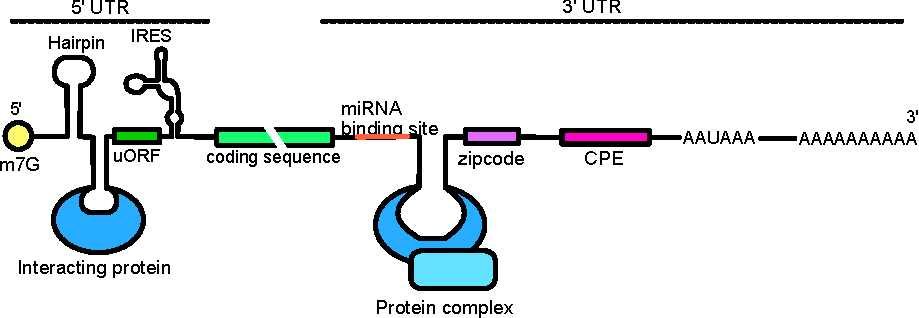
\includegraphics{./figures/UTRFeatures_2.pdf}
  \caption{ Schematic overview of mRNA - mRNA consists of a coding sequence, 5' and 3' untranslated regions flanking the coding sequence, a 5' cap and a poly-(A)-tail. Located within the 5' and 3' untranslated region are post-transcriptional regulatory elements that can influence gene expression. uORF; upstream open reading frame; IRES, internal ribosome entry site; CPE, cytoplasmic polyadenylation site; AAUAAA, polyadenylation signal. See section \ref{regmRNA} for details on these elements.
 \label{fig:UTRFeat}}
\end{figure}

The 5' end of mRNAs contain a 7-methyl-guanylate (m7G) cap that is important for translation initiation, while the 3' end has a poly-A tail protecting the mRNA against degradation (Grifo et al., 1983; Wilusz et al., 2001). Multiple different mRNA variants (also called isoforms) from the same gene can exist. Isoforms may arise due to alternative transcription start site usage or a process called alternative splicing. Isoforms can co-exist at the same time and have differing properties that can perform distinct functions (Joly Anne-Laure et al., 2018). Furthermore, alternative splicing may result in isoforms with different 5' UTRs. This leads to altered translation of mRNAs encoding for the same protein (Floor et al., 2016; Jewer et al., 2020).

\subsection{The steps of mRNA translation} \label{translation}

In eukaryotes, mRNA translation occurs in the cytoplasm for the vast majority of protein coding mRNAs. However, a small subset of mRNAs encoded by mitochondrial DNA is translated in the mitochondria (D'Souza et al., 2018). mRNA translation is a process that consists of several steps: initiation, elongation, termination and ribosome recycling (\emph{see figure \ref{fig:doodlemRNASteps}}). These steps will be discussed in detail below.

\begin{wrapfigure}{o}{1\textwidth}
  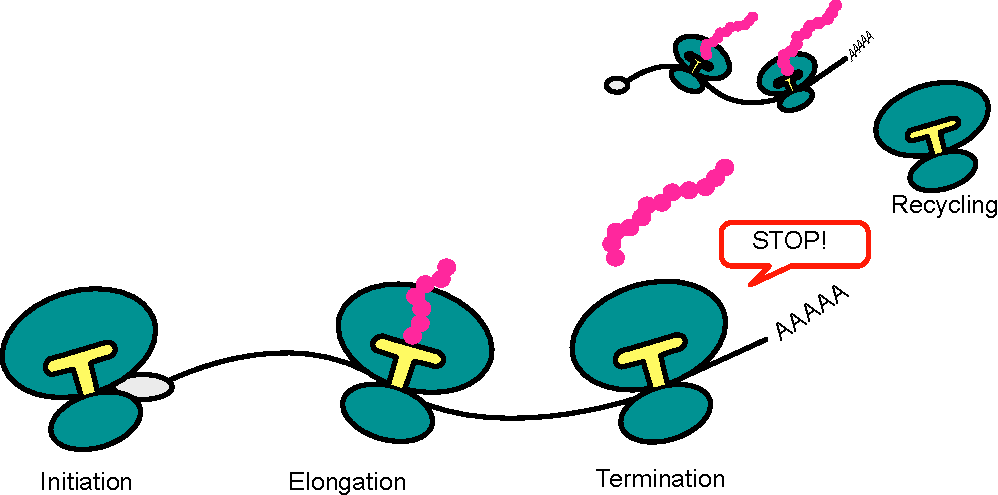
\includegraphics{./figures/doodleTranslation.pdf}
  \caption{mRNA translation initiation, elongation, termination and ribosome recycling steps - The ribosome binds to the mRNA and initiates scanning for a start codon (AUG). The elongation phase incorporates amino acids into a polypeptide chain (i.e. the protein product). Once a stop codon (e.g. UGA) is detected, the ribosome terminates translation and releases the polypeptide chain. The ribosome can then be recycled to participate in the translation of another mRNA or reinitiate on the same mRNA. Green ovals represent the ribosomal subunits. Within the ribosome the E, P and A-sites are indicated with yellow boxes (see section \ref{elongation} for details). Polypeptide chains are depicted as a series of pink balls. Orange crosses represent transfer RNAs (tRNA) (see section \ref{elongation} and \ref{tRNA} for more details on tRNAs).  \label{fig:doodlemRNASteps}}
\end{wrapfigure}
\clearpage

\subsubsection{Initiation} \label{initiation}

In eukaryotes, 5' cap-dependent initiation of mRNA translation consists of multiple stages. First, a ternary complex (TC) consisting of guanosine-tri-phosphate (GTP) bound eukaryotic initiation factor (eIF) 2 and methionine-initiator transfer RNA (met-tRNAi) is formed. This is followed by formation of the 43S pre-initiation complex (PIC). The PIC consists of a 40S ribosome subunit, the TC and, translation initiation factors eIF1, eIF1A, eIF3 and, eIF5 (Asano et al., 2000). mRNAs then undergo ``activation.'' Here, the 5' cap proximal structure is bound by eIF4F. eIF4F is the 5' cap binding complex consisting of: the 5' cap binding protein eIF4E, the RNA helicase eIF4A and, a scaffold protein eIF4G (Grifo et al., 1983). The Poly (A) binding protein (PABP) binds to the poly(A) tail of the 3' UTR and causes circularisation of the mRNA. The circularisation improves stability of the mRNA and aids in recruitment of translation initiation factors (Ivanov et al., 2016). Upon mRNA recruitment, the ATP-dependent eIF4A helicase activity of the eIF4F complex facilitates scanning of 43S PIC along the 5'UTR together with eIF4B and eIF4H. Recognition of the translation initiation codon (AUG) induces formation of the 48S initiation complex. Once the initiation codon (AUGi) is reached, displacement of eIF1 occurs which allows eIF5 to hydrolyse eIF2-bound GTP. The 60S ribosomal subunit then joins the 40S ribosomal subunit which causes the release of eIF2-GDP and other initiation factors (eIF1, eIF3, eIF4B, eIF4F and eIF5). Subunit joining is mediated by eIF5B. After subunit joining the 80S ribosome is formed and the elongation process starts (\emph{see figure \ref{initiation}}) (Asano et al., 2000; Alan G. Hinnebusch, 2006; Jackson et al., 2010). A mechanism for cap dependent translation initiation that is independent of eIF4E has been described. Here, eIF3d binds the 5' cap of mRNAs containing an RNA element that blocks eIF4E binding A. S. Y. Lee et al. (2016). Next to 5'cap-dependent initiation, mRNA translation can also be initiated in a 5' cap-independent manner, e.g.~via the internal ribosome entry site (IRES) (\emph{see figure \ref{fig:UTRFeat}}). Mechanisms for 5' cap-independent mRNA translation initiation are extensively reviewed elsewhere (Lacerda et al., 2017; Shatsky et al., 2018).

\subsubsection{Elongation} \label{elongation}

The 80S ribosome contains three sites important for decoding an mRNA: the aminoacyl (A), peptidyl (P) and exit (E) sites. During elongation in eukaryotes, aminoacytelated tRNAs are delivered to the A-site in a ternary complex with eukaryotic elongation factor (eEF) 1A and GTP. If the tRNA is cognate to the codon in the A-site of the ribosome, GTP bound to eEF1A is hydrolysed. This causes eEF1A to release and accommodates the aminoacetylated tRNA in the A-site. This is followed by a peptidyl transferase reaction. This reaction forms the peptide bond between the peptidyl tRNA in the P-site and amino group of the aminoacyl-tRNA in the A-site (aa-tRNA) and is catalysed by 60S ribosomal subunit. After the peptide bond is formed a translocation step occurs through eEF2-GTP hydrolysis. The translocation step encompasses that the deacetylated tRNA currently in the P-site moves into the E-site. Likewise, the peptidyl tRNA in the A-site moves to the P-site. Which leaves the A-site open for other aa-tRNAs. The deacytelated tRNA in the E-site is then released from the ribosome (Dever et al., 2012). This process is repeated until a stop codon (UAA, UGA or UAG) enters the A-site of the ribosome.

\begin{figure}[ht]
\centering
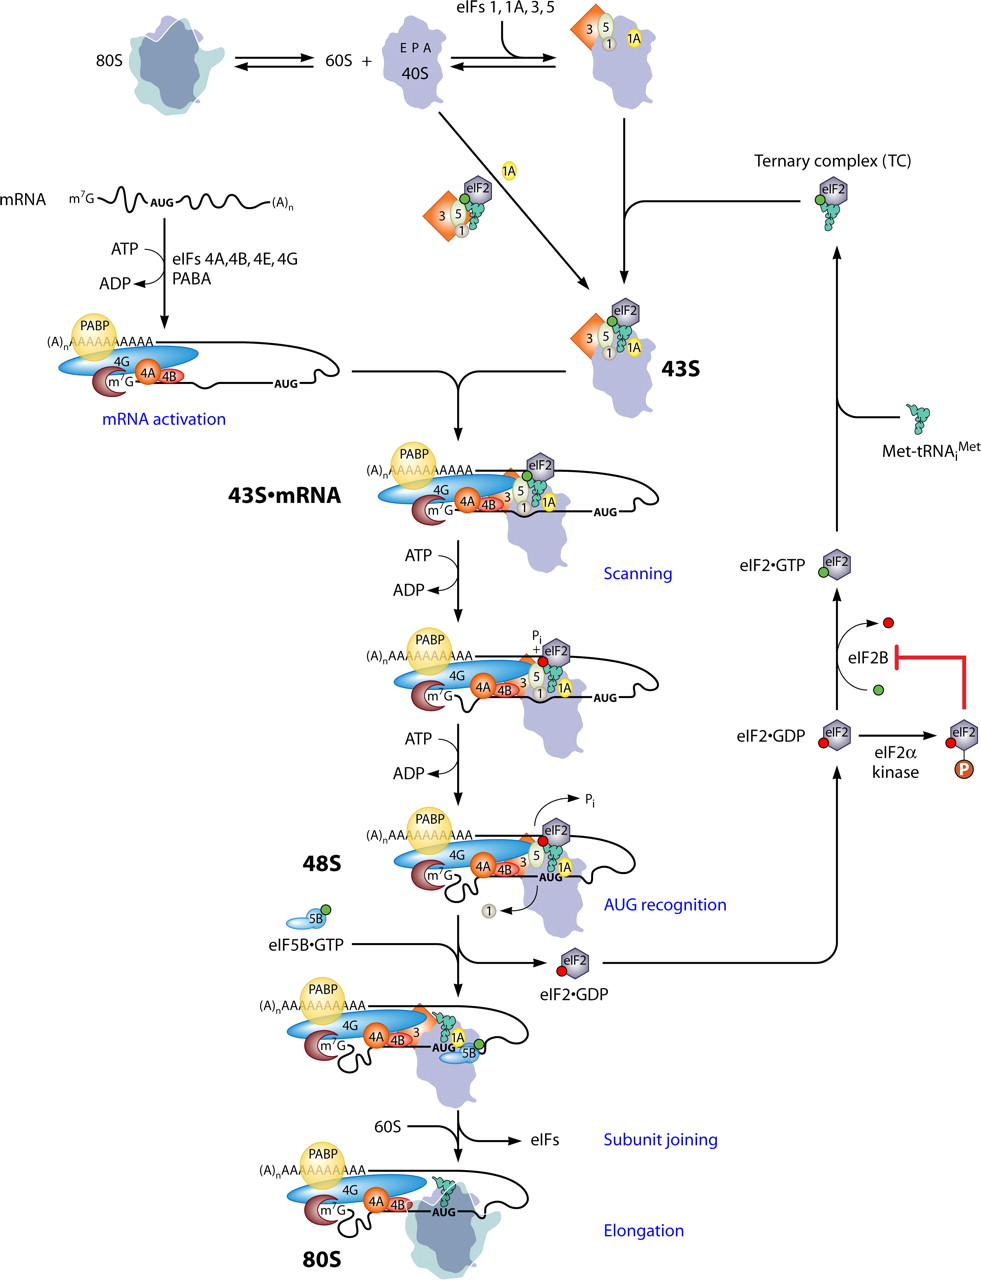
\includegraphics[width=1.0\linewidth,height=0.8\textheight]{./figures/initiation.jpg} 
  \caption{Pathway of eukaryotic translation initiation via ribosomal scanning. Reprinted with permission. Cold Spring Harb Perspect Biol. 2012 Oct; 4(10): a011544.doi: 10.1101/cshperspect.a011544.© 2012 Cold Spring Harbor Laboratory Press.
  \label{fig:initiation}}
\end{figure}

\clearpage

\subsubsection{Termination and recycling} 
\begin{wrapfigure}{r}{.4\textwidth}
  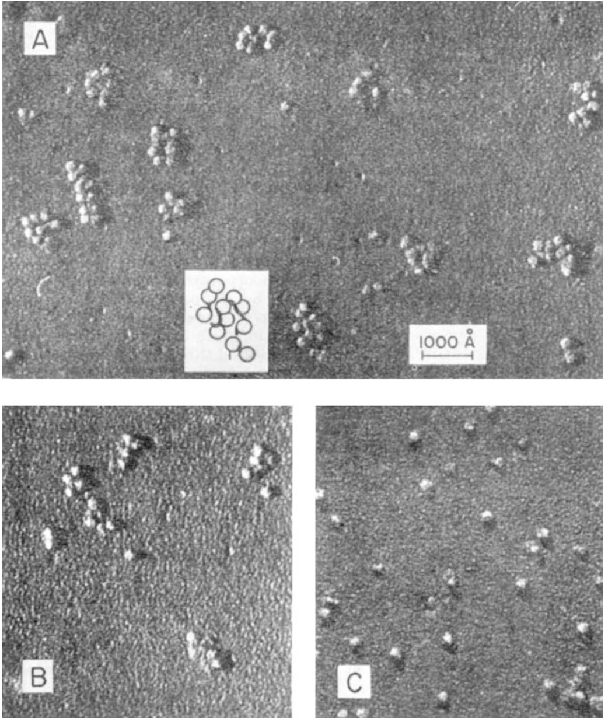
\includegraphics{./figures/polysome.pdf}
  \caption{Electromicrongraph of ribosomes extracted from different positions along a sucrose gradient used for polysome fractionation (A-C). Multiple ribosomes bound to the same mRNA can be observed. For details on polysome fractionation see section \ref{exptMethod}. Reprinted with permission. DR. T. STAEHELIN et. al. Nature.1963 Aug 31;199:865-70.doi: 10.1038/199865a0. Copyright © 1963, Nature Publishing Group.
 \label{fig:polysomes}}
\end{wrapfigure}

mRNA translation termination is facilitated by two eukaryotic release factors (eRF), eRF1 and eRF3-GTP (Alkalaeva et al., 2006; Stansfield et al., 1995). The eRF1:eRF3-GTP complex binds to the A-site of the ribosome upon recognition of a stop codon. This causes an hydrolysis event resulting in a conformational change and release of the polypeptide chain. eRF1 and the ATP binding cassette protein (ABCE1) together promote the splitting of the 60S and 40S subunits after which they can be recycled (Hellen, 2018; Pisarev et al., 2010).

\subsection{Translation efficiency} \label{transEff}

Each ribosome synthesises a single protein during translation of an mRNA assuming it is not prematurely terminated. It has been known since the `60s that translation of an mRNA occurs via multiple bound ribosomes (polysomes) simultaneously (\emph{see figure \ref{fig:polysomes}A-C}) (Staehelin et al., 1963; Warner et al., 1962). Therefore, the translation efficiency of an mRNA depends on the number of ribosomes it is associated with. Experimental methods like polysome profiling and ribosome profiling are used to study translation efficiency by measuring the number of ribosomes bound on an mRNA (\emph{explained in detail in section \ref{exptMethod}}). While all steps of translation can affect the translation efficiency of an mRNA, it is thought to most commonly be regulated at the initiation step (Dever et al., 2012; Jackson et al., 2010; Richter et al., 2015). This is supported by findings using polysome profiling in yeast that was cultured in nutrient rich medium where initiation was rate-limiting for most mRNAs (Arava et al., 2003). Furthermore, a recent ribosome profiling study assessed transcriptome-wide elongation rates. This revealed a similar rate of elongation for mRNAs of different classes, e.g.~mRNAs with differences in 5' UTR characteristics (Ingolia et al., 2011). The next section will go further into detail how translation initiation and elongation can be regulated.
\newline

\section{Regulation of mRNA translation} \label{regmRNA}

mRNA translation is the most energy consuming process in the cell. In a study using concanavalin A stimulated rat thymocytes, it was estimated that translation accounts for \textasciitilde20\% of the cellular energy consumption (Buttgereit et al., 1995). The high energy consumption of mRNA translation and its central role in the gene expression pathway requires it to be tightly regulated.

Regulation of translation can be exerted at a global level, i.e.~regulation of a large set of mRNA simultaneously. Global regulation of mRNA translation can be achieved by, e.g.~perturbations of major signalling pathways impinging on mRNA translation. Regulation of mRNA translation is that it can affect specific mRNA populations selectively. Selective translational regulation acts on characteristics of mRNAs, e.g.~through 5' UTRs or RNA binding proteins (RBP) that bind to the 3' UTRs (\textbf{see figure \ref{fig:UTRFeat}}) (Leppek et al., 2018). Furthermore, regulation of initiation factors can also regulate translation selectively Gandin, Masvidal, Hulea, et al. (2016). Below we will discuss multiple mechanisms that regulate mRNA translation globally or selectively.

\subsection{mTOR} \label{mTOR}

mTOR is a conserved Ser/Thr kinase and is found in two structurally and functionally distinct complexes, mTORC1 and mTORC2 (Pearce et al., 2007; Saxton et al., 2017). In a growth promoting environment mTOR regulates cell metabolism to increase protein synthesis, lipids and nucleotides, while suppressing catabolic pathways, e.g.~autophagy. mTORC2 promotes survival via signalling through protein kinase A (AKT), anabolic metabolism, and cytoskeleton regulation Zoncu et al. (2011).

mTORC1 activity is modulated via hormone and growth factor signalling, e.g.~insulin and insulin-like growth factor (IGF1). This signalling is predominantly mediated through the phosphoinositide 3-kinase (PI3K) / AKT pathway. PI3K activation generates phosphatidylinositol-3,4,5-trisphosphate (PIP3). Phosphatase and tensin homologue (PTEN) can counteract this by hydrolysis of PIP3 to phosphatidylinositol 4,5-bisphosphate (PIP2). PIP3 recruits phosphoinositide-dependent kinase 1 (PDK1) and AKT to the plasma membrane. At the plasma membrane AKT is activated through phosphorylation of PDK1. AKT in turn increases activity towards its substrate tuberous sclerosis complex (TSC). TSC consists of a scaffold protein, TSC1, and a GTPase, TSC2. TSC negatively regulates mTORC1 activity. This negative regulation occurs through hydrolysis of Ras homologue enriched in brain (Rheb) that leads to its inactivation. Rheb binds to mTOR to promote its activity (\emph{see Figure \ref{fig:mtorsignal}}). Furthermore, several cross-talk mechanism with other pathways (e.g.~RAS/ERK) have been shown to lead to mTORC1 activation (reviewed in (Reuben J. Shaw et al., 2006)). The mechanisms of mTORC2 activation are less well understood.

The PI3K pathway is involved in oncogenic signalling and under investigation as therapeutic target in cancer (Hilger et al., 2002; Yang et al., 2019). In several cancers (e.g.~breast, lung, prostate and colon) the gene encoding the catalytic p110\(\alpha\) subunit of PI3K (PI3KCA) is frequently mutated or amplified (J. W. Lee et al., 2005; D. A. Levine et al., 2005; Samuels et al., 2004). The E545K mutation leads to a reduced inhibitory effect of the regulatory p85 subunit on PI3KCA. In \textbf{study 3}, we investigate oncogenic signalling via the PI3K pathway activated by insulin. Here, were focus on the role of mTOR in mediating the effects of insulin on gene expression in the MCF7 breast cancer cell line that harbours the E545K mutation (Schneck et al., 2013). Hyperactivity of PI3K/AKT signalling has been reported in multiple cancers and has been linked to anti-cancer therapy resistance (Pópulo et al., 2012; Salaroglio et al., 2019; Tan et al., 2013). Furthermore, both PTEN and the TSC act as tumour suppressors and are frequently mutated in cancer (Mak et al., 2004; Song et al., 2012). Therefore, mTOR has become a focus of anti-cancer therapy by either targeting mTORC1 or using dual inhibitors for PI3K and mTOR (Bhat et al., 2015).
\clearpage

\begin{figure}[ht]
 \centering
  \includegraphics{./figures/mTORsignal.jpg}
  \caption{Schematic representation of mTOR signalling to the translational machinery. Philippe P. Roux, and Ivan Topisirovic Mol. Cell. Biol. 2018; doi:10.1128/MCB.00070-18. Reprinted with permission. Copyright © 2018, American Society for Microbiology
 \label{fig:mtorsignal}}
\end{figure}

mTOR also fulfills a central role in metabolic signalling. Here, mTOR integrates signals arising through amino acid availability, glucose metabolism and cellular oxygen levels. For example, increased amino acid availability induces relocalisation of mTOR into proximity of Rag GTPases leading to its activation through Rheb (Sancak et al., 2008). Furthermore, Glucose deprivation leads to increased adenosine-mono-phosphate kinase (AMPK) signalling via serine/threonine kinase 11 (LKB1) (Kimball, 2006; Sanders et al., 2007; R. J. Shaw, 2009). In turn, AMPK phosphorylates TSC2 leading to its activation (Kimball, 2006). LKB1 mutations have been found in cancer and are being considered as targets in anti-cancer therapy (Zhao et al., 2014). Hypoxia also inhibits mTOR via regulated in development and DNA damage response 1 (REDD1) which stabilises the TSC (Brugarolas et al., 2004). While hypoxia (i.e.~deprivation of oxygen) inhibits protein synthesis in normal cells, in breast cancer, protein synthesis appeared not to be significantly inhibited during hypoxia which is attributed to uncontrolled mTOR signalling (Connolly et al., 2006).

In cancer, cellular metabolism, proliferation as well as growth are often dysregulated (Hanahan et al., 2011). Given the central of mTOR governing proliferation, growth, and metabolism it is vital to comprehensively understand mTOR signalling in this disease (Roux et al., 2018).

\subsubsection{Global regulation of translation via mTOR}

Well studied downstream targets of mTOR for the regulation of mRNA translation are 4E-binding proteins (4E-BP) and ribosomal protein S6 kinases (S6Ks). mTOR phosphorylates 4E-BP leading to the release of eIF4E that then can engage in eIF4F complex formation (Gingras et al., 1999). Therefore, inhibition of mTOR leads to a down regulation of 5' cap-dependent mRNA translation.

S6Ks have been shown to regulate phosphorylation of multiple components of the translation machinery, e.g.~ribosomal protein S6 (rpS6), programmed cell death protein 4 (PDCD4), eEF2 kinase and eIF4B. S6K phosphorylates rpS6 which has been implicated in the regulation of cellular growth and protein synthesis (Ruvinsky et al., 2005). Furthermore, S6K/rpS6 signalling was suggested to be involved in ribosome biogenesis. Another S6K target is eEF2 kinase which phosphorylates and inhibits eEF2, thus attenuating elongation rates. (X. Wang et al., 2001). MTORC1 phosphorylates and inhibits eEF2K either directly or via S6Ks. Furthermore, phosphorylation of PDCD4 by S6K triggers its degradation. PDCD4 blocks eIF4G-eIF4A interactions repressing eIF4A activity and cap-dependent mRNA translation (Dorrello et al., 2006; Göke et al., 2002). Lastly, phosphorylation of eIF4B by S6K is suggested to stimulate the unwinding activity of eIF4A (Rogers et al., 2001).

Collectively, through acting on its downstream targets, mTOR regulates translation globally via a number of mechanisms.

\subsubsection{Selective or "mTOR sensitive" regulation of translation}

\paragraph{Terminal oligo pyrmidine mRNAs}

Selective or ``mTOR sensitive'' regulation of translation can act on a terminal oligo pyrimidine (TOP) motif in the 5' UTR of mRNAs. This TOP motif consists of a C followed by a stretch of 4-15 pyrimidines directly after the 5' cap. TOP mRNAs show near complete dissociation from ribosomes under conditions when mTOR is inhibited and are enriched for genes encoding for components of the translation machinery (Meyuhas, 2000; Thoreen et al., 2012; Yamashita et al., 2008). Recent works indicate the importance of La ribonucleoprotein domain family member 1 (LARP1) in regulation of TOP mRNAs with contradictory findings (Fonseca et al., 2015; Hopkins et al., 2016; Jia et al., 2021; Maraia et al., 2017). A panel of researches was asked to evaluate these findings, which led to the establishment of a model for translational regulation via LARP1 (Berman et al., 2021). According to this model, LARP1 binds to the 5' mRNA cap of TOP mRNAs via its DM15 domain. Binding of DM15 represses translation of TOP mRNAs by obstructing eIF4E binding and occurs in instances where mTOR activity is reduced. Under conditions where mTOR is active, DM15 is phosphorylated by mTOR. This causes DM15 to release the 5' cap. However, the la domain of LARP1 remains bound to the 3' UTR. The still bound la domain stabilises the mRNA to facilitate translation (Berman et al., 2021). Other instances of selective translation by mTOR are explained in the next section.

\paragraph{Selective regulation through members of the eIF4F complex} \label{sel4F}

As mentioned above, the eIF4F complex consists of eIF4E, eIF4A and eIF4G and is required for cap-dependent mRNA translation (Alan G. Hinnebusch, 2014). The availability of the eIF4F complex is limited under basal conditions due to that eIF4E is bound by 4E-BPs. Therefore, under basal conditions mRNAs must compete for access to components of the translation machinery. Such competition is affected by characteristics of 5' UTRs that introduce variation to how well mRNAs can be translated. Benedetti et. al.~derived and expanded on a model for mRNA competition originally proposed by Lodish (De Benedetti et al., 2004 ; Lodish, 1974). Herein, ``strong'' mRNAs are widely expressed and, represent the majority of cellular mRNAs and are characterised by optimally long and unstructured 5' UTRs, e.g.~\(\beta\)-actin. An optimal 5' UTR length of 70-150 nucleotides was proposed by Kozak (Kozak, 1987). On the other hand, ``weak'' mRNAs have long and structured 5' UTRs. ``Weak'' mRNAs encode for potent growth and survival factors, e.g.~c-Myc, ornithine decarboxylase (ODC1) and vascular endothelial growth factor (VEGF). Translation of ``strong'' mRNAs would remain effective in conditions where eIF4F complex availability would be limited. However, ``weak'' mRNAs show sensitivity to eIF4F availability which is dependent on eIF4E expression and/or availability (Graff et al., 2008). Elevated eIF4E expression and/or availability due to increased mTORC1 activity and consequent inhibition of 4E-BPs are common in cancer and drives malignancy due to selective induction of translation of tumour promoting mRNAs (De Benedetti et al., 2004).

In addition to eIF4E, other eIF4F subunits have been shown to also selectively impact mRNA translation. Therein, mRNAs dependent on eIF4A showed characteristics of ``weak'' mRNAs, i.e.~these mRNAs had long and structured 5' UTRs (Rubio et al., 2014; Waldron et al., 2018; Wolfe et al., 2014). Structural elements in the 5' UTRs include classical hairpins formed through Watson-Crick base pairing (\emph{see Figure \ref{fig:UTRFeat}}) (Leppek et al., 2018). Other structures formed via hoogsteen base pairing have also been proposed to regulate eIF4A dependent mRNA translation (Wolfe et al., 2014). These structures are called G-quadruplexes. G-quadruplexes are stable structures formed by stacking two or more G-tetrads (Kwok et al., 2017). However, whether G-quadruplexes form in RNA is still debated (Biffi et al., 2014; Guo et al., 2016; Laguerre et al., 2015; Weldon et al., 2016). Formation of G-quadruplex structures is predicted based on occurrences of \(GGC_4\) motif repeats in the 5' UTR of mRNAs (Singh et al., 2021; Wolfe et al., 2014). Indeed, multiple studies report enrichment of \(GGC_4\) motifs in mRNAs whose translation is dependent on eIF4A (Modelska et al., 2015; Rubio et al., 2014; Singh et al., 2021; Waldron et al., 2018). However, Waldron et al.~show that \(GCC_4\) motifs fail to form G-quadruplexes in their reporter mRNA system. The authors concluded that eIF4A dependence of mRNAs with \(GGC_4\) motifs enriched in their 5' UTR was likely mediated by classical hairpin-like structures (Waldron et al., 2018). In addition, in Rubio et al.~one third of eIF4A-dependent mRNAs exhibited multiple 5' UTR variants, while for eIF4A-independent mRNAs this was \textless{} 1\% (Rubio et al., 2014). Translation of mRNAs with different 5' UTR variants has recently been implicated to drive cancer cell plasticity towards more ``stem cell-like'' phenotypes during hypoxia (Jewer et al., 2020). In addition, eIF4A inhibitors with different mechanisms of action have been shown to exert different impact on the translatome. Hippuristanol inhibits RNA interaction by selective binding to eIF4A (Bordeleau et al., 2006; Lindqvist et al., 2008). In contrast rocaglates and their derivatives, e.g.~silvestrol and CR-1-31-B, clamp eIF4A on polypurine sequences on the mRNA (Iwasaki et al., 2016).

Recently, a more nuanced picture for translation of mRNAs sensitive to inhibition of components of the eIF4F complex has been reported (Gandin, Masvidal, Hulea, et al., 2016). Therein, a comparison of treatments with a mTOR and eIF4A inhibitors was evaluated. This revealed that non-TOP mTOR-sensitive mRNAs encompass two functionally distinct sets of mRNAs. These sets were characterised by different 5' UTR features. Here, one subset showed less sensitivity to eIF4A but more so to eIF4E (here after referred to as mTOR-eIF4E sensitive mRNAs). mTOR-eIF4E sensitive mRNAs contain very short 5' UTRs (\textless{} 40 nt) and encode for proteins in metabolic functions. The other subset was sensitive to both eIF4E and eIF4A (hereafter referred to as mTOR-eIF4A sensitive). mTOR-eIF4A sensitive mRNAs were characterised by long and structured 5' UTRs that encode for pro-survival proteins. The authors concluded that inhibition of mTOR-eIF4A dependent programs would lead to cytotoxic effects. Whereas, inhibition of mTOR-eIF4E mRNAs would lead to metabolic dormancy and a cytostatic effect (Gandin, Masvidal, Hulea, et al., 2016). The difference in cytostatic and cytotoxic effects was attributed to that eIF4A inhibition leads to continuous expression of proteins involved in respiration. However, expression of proteins protecting mitochondrial integrity would be reduced. Thus, leading to apoptosis. In contrast, inhibition of mTOR activity would impact protein expression of both subsets simultaneously, leading to metabolic dormancy.

\subsection{The integrated stress response}

The integrated stress response (ISR) is a pathway activated through kinases responding to various stress signals. These kinases include: Protein kinase R-like endoplasmic reticulum kinase (PERK) activated by misfolded peptides in the endoplasmatic reticulum (ER); Heme regulated eIF2alpha kinase (HRI) activated during heme deficiency; Protein kinase R (PKR) which is activated in response to certain viral infections by binding to double-stranded RNA (dsRNA); and general control nonderepressible 2 (GCN2) which is activated when cells are deprived of amino acids (Dmitry E. Andreev et al., 2015; Guan et al., 2017; Kapur et al., 2017; Lemaire et al., 2005; Taniuchi et al., 2016).

\subsubsection{Global and selective regulation of translation via the ISR}

Similar to mTOR signalling, regulation of translation via the ISR is achieved at a global and selective level. During the ISR the \(\alpha\) subunit of eIF2 is phosphorylated. Phosphorylated eIF2\(\alpha\) directly engages the guanine nucleotide exchange factor eIF2B and prevents conversion of inactive eIF2-GDP to active eIF2-GTP needed for met-tRNAi incorporation in the TC. This reduces TC availability and causes a global downregulation of mRNA translation (Sonenberg et al., 2009) (\emph{see figure \ref{fig:initiation}}). While global translation is reduced upon ISR, translation of a selective subset of mRNA with upstream open reading frames (uORFs) is increased. A uORF is a reading frame that originates in the 5' UTR of an mRNA upstream of the coding ORF (cdsORF) (\emph{see Figure \ref{fig:UTRFeat}}). uORFs can be out of frame with the cdsORF and, when translated, lower the expression of the cdsORF (Kozak, 1984). Activating transcription factor 4 (ATF4), that regulates expression of stress response genes, contains multiple uORFs of which one partially overlaps with the cdsORF. Under normal conditions ATF4 translation is initiated at uORF1 and reinitiation at uORF2 occurs. The overlap of uORF2 with the cdsORF causes ribosomes to synthesise protein from uORF2 thereby inhibiting the translation of the cdsORF. Limitation of TC availability during ISR causes longer ribosome scanning times leading to that ribosomes scan past uORF2 and initiate at the cdsORF (i.e.~delayed reinitiation) (Pakos-Zebrucka et al., 2016).

Ribosome profiling studies indicate that 50\% of mammalian mRNAs harbour uORFs (\emph{see section \ref{exptMethod} for details on ribosome profiling}). mRNAs containing uORFs include oncogenes and transcripts important in differentiation and cell cycle (Calvo et al., 2009; Ingolia et al., 2011). Apart from delayed reinitiation, uORF translation can also be regulated by ``leaky scanning.'' The surrounding sequence of the uORF is important for initiation of translation. An AUG in the classical Kozak context (i.e.~RNN\textbf{AUG}G) is most efficient for translation initiation due to better recognition by the met-tRNAi (Calvo et al., 2009; Kozak, 1986). Unfavoured flanking sequences of the AUG can cause the ribosome to scan past the AUG, this process is called ``leaky scanning.'' An example of this is DNA-inducible gene 34 (GADD34) which increases its translation upon ER stress, i.e.~a condition where eIF2\(\alpha\) is phosphorylated. In humans, GADD34 contains two uORFs separated by 30 nucleotides (Y.-Y. Lee et al., 2009). In contrast to the uORFs in ATF4, the uORFs in GADD34 are too close together to allow for reinitiation. Under basal conditions uORF2, which has a poor Kozak context, represses translation of the cdsORF. However, under stress causing eIF2\(\alpha\) phosphorylation, ribosomes scan past uORF2 to translate the cdsORF (Young et al., 2015). Lastly, structural elements in proximity of the uORF can also influence its translation (Ruan et al., 1994).

\subsection{Regulation of mRNA translation by tRNAs} \label{tRNA}
\begin{wrapfigure}{r}{0.6\textwidth}
  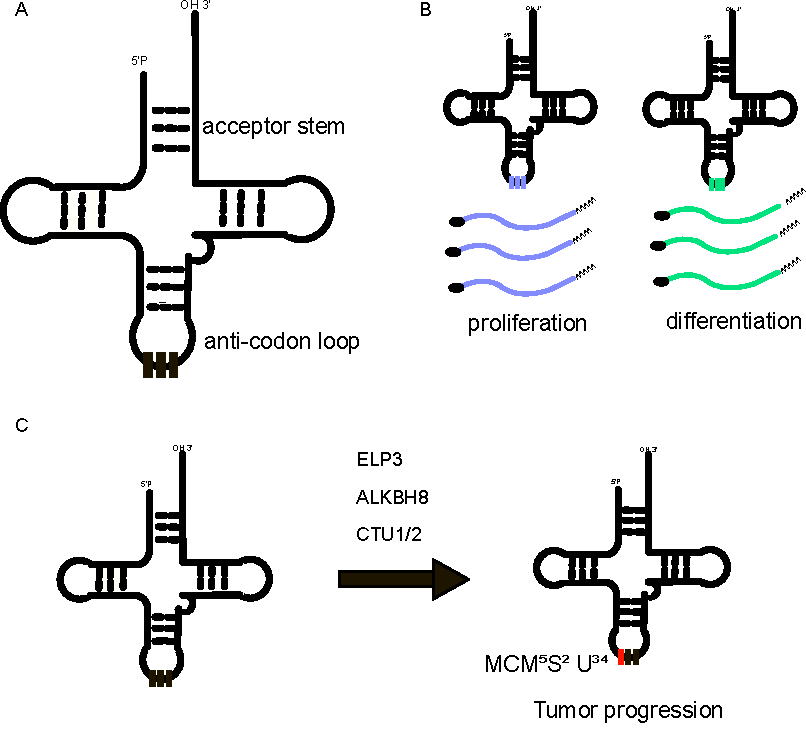
\includegraphics{./figures/tRNA.pdf}
  \caption{ Schematic representations of (A) the tRNA cloverleaf structure with indicated anti-codon and amino acid acceptor sites;  (B)  the proliferation and differentiation mRNAs dependent on distinct tRNA subsets; (C) the U34 wobble position and the catalytic enzymes involved in this modification that is implied in tumour progression.
 \label{fig:tRNA}}
\end{wrapfigure}

As touched upon earlier, tRNAs are an essential part of the translation machinery that carry the amino acids to the ribosome. In eukaryotes, tRNAs consist of a 76-90 long nucleotide sequence set into a ``cloverleaf'' structure forming several loops (Sharp et al., 1985) (\emph{see figure \ref{fig:tRNA}}). The acceptor stem binds the amino, while the anti-codon loop binds to the mRNA within the ribosome via classical Watson-Crick base pairing (Watson et al., 1953). Multiple codons can encode for the same amino acid (synonymous codons), however the availability of the tRNAs for different codons may vary which can influence elongation rates and thus protein synthesis.

This supply ( i.e.~tRNA availability) and demand (i.e.~codon composition) relationship has been found to vary across different cellular states, e.g.~proliferation and differentiation. Gingold et. al.~observed two different tRNA subsets. One subset is induced when proliferation is stimulated and is otherwise repressed. And the other subset increases expression when differentiation is induced and is repressed otherwise (\emph{see figure \ref{fig:tRNA}}). Both tRNA subsets match the codon demand of the transcriptome under their respective cellular state (Gingold et al., 2014). This model has been disputed and it was proposed that the observed differences may be attributed to GC content in the mRNA (Rudolph et al., 2016). Nevertheless, aberrant tRNA expression and codon usage have been reported in cancer (Z. Zhang et al., 2018). Furthermore, a comprehensive study using small RNAseq (e.g.~for identification of tRNAs) and protein samples across 17 tissues reported a tRNA signature stratified by proliferation marker Ki67 staining. The identified tRNA signature has implications for patient survival (Hernandez-Alias et al., 2020). Therefore, while a consensus on proliferation specific tRNA subsets might not have been reached, emerging evidence implicates a role thereof in cancer (Gingold et al., 2014; Hernandez-Alias et al., 2020; Z. Zhang et al., 2018). For instance, increased expression of \(tRNA_{CCG}^{Arg}\) and \(tRNA_{UUC}^{Glu}\) has been observed in breast cancer cell lines and are proposed to drive metastasis (Goodarzi et al., 2016).

Others reported of a role for tRNAs in cancer attributed to tRNA modifications, specifically at the highly conserved U34 anti-codon (wobble) position (El Yacoubi et al., 2012; Lorent et al., 2019; Rapino et al., 2017). The ability to wobble was proposed by Francis Crick and refers to non-Watson-Crick base pairing of tRNA anti-codons (F. H. Crick, 1966). This enables a smaller set of tRNAs (41-55 in eukaryotes) to encode for the 64 possible codon combinations (Goodenbour et al., 2006). In mammals, the U34 modification catalytic cascade involves the acetyltransferase Elongator (ELP3), the methyltransferase TRM9-like domain of Alkylation repair homolog 8 (ALKBH8), and the urmylation (URM) pathway. The URM pathway includes the cytosolic thiouridylase homolog 1 and 2 (CTU1/CTU2) (Kalhor et al., 2003; Karlsborn et al., 2014). These enzymes ultimately modify the U34 position into 5-methoxycarbonyl-methyl-2-thiouridine (\(mcm^5s^2U\)) which ensures cognate codon recognition. This modification is thought to occur in tRNAs with a U in the wobble position, e.g.~\(tRNA^{UUU}\), \(tRNA^{UUC}\), \(tRNA^{UUG}\), \(tRNA^{UCC}\), and \(tRNA^{UCU}\) (\emph{see figure \ref{fig:tRNA}}).

Loss of the ability to modify U34 has been shown to reduce translation elongation rates with varying effects on protein expression (Deng et al., 2015; Nedialkova et al., 2015; Zinshteyn et al., 2013). While in some cases U34 dependent signalling led to ribosome stalling resulting in protein aggregates and increased stress (Nedialkova et al., 2015; Zinshteyn et al., 2013), others reported a subtle downregulation of proteins encoded by mRNAs requiring U34-modified tRNAs (Deng et al., 2015). U34 modification dependent tRNAs have been shown to play a role in cancer. For example, ELP3 is important in tumour initiation in intestinal epithelia and promotes breast cancer invasion as well as progression to metastasis (Delaunay et al., 2016; Ladang et al., 2015).

\subsection{RNA binding proteins and trans-acting factors}

The UTRs of an mRNA contain sequence elements to which small RNA and RNA binding proteins (RBPs) bind and exert translational regulation (\emph{see figure \ref{fig:UTRFeat}}).

\subsubsection{microRNAs}

microRNAs (miRNA) are a class of small non-coding RNA. The precise role and mechanisms of regulation of translation by miRNAs are still under active investigation (Oliveto et al., 2017). However, miRNAs can directly bind to other mRNAs and silence them which is accomplished through translational repression or destabilisation (Jonas et al., 2015). Regulation of gene expression by miRNAs has been observed in cancer. Here, miRNAs have been implicated to promote tumorigenesis or act as tumour suppressors (Muniyappa et al., 2009; Nagpal et al., 2015; Sampson et al., 2007; Tian et al., 2010).

\subsubsection{RNA binding proteins}

RBPs are a class of proteins involved in many regulatory steps of gene expression and account for \textasciitilde7.5\% of the protein coding genes. RBPs bind to elements in the 3' UTRs, e.g.~the poly (A) tail. One RBP binding the poly(A) tail is PABP. As explained in \emph{section \ref{initiation}} PABP is involved in mRNA translation initiation and stabilisation of the mRNA (Afonina et al., 2014; Amrani et al., 2008) (\emph{see also figure \ref{fig:initiation}}).

Another site in the 3' UTR is the U-rich cytoplasmic polyadenylation (CPE) site to which cytoplasmic polyadenylation element binding proteins (CPEBs) can bind (\emph{see Figure \ref{fig:UTRFeat}}). Studies in \emph{Xenopus} oocytes indicate that CPEB associates with a non-canonical poly(A) polymerase (Gld2) and a poly(A) deadynelase (PARN). PARN has a higher activity than Gld2 and thus binding of CPEB to an mRNA leads to shortening of the Poly(A) tail (Barnard et al., 2004). However, hormonal stimulation leading to CPEB phosphorylation removes PARN from the complex. Removal of PARN promotes poly(A) tail elongation through Gld-2 (Kim et al., 2006). Furthermore, in \emph{Xenopus} oocytes, CPEB associates with an eIF4E binding protein, i.e.~maskin. Maskin bound to eIF4E prevents eIF4F complex formation which represses mRNA translation (Ivshina et al., 2014; Stebbins-Boaz et al., 1999). Therefore, CPEBs can regulate translation by altering 3' UTR lengths and are involved in translational repression by blocking eIF4E association with the 5' cap in \emph{Xenopus} oocytes. While the role of CPEB mediated regulation has been described mostly in \emph{Xenopus} oocytes, dysregulation of CPEBs has been observed in glioblastoma, colorectal and pancreatic cancer (Chang et al., 2014; Ortiz-Zapater et al., 2011; Villanueva et al., 2017).

Another important RBP implicated in regulation of translation is Human antigen R (HuR). HuR preferentially binds to AU-rich sequences in the 3' UTR, acts as a stabilising agent and is involved in RNA-processing (Baou et al., 2011; Fan et al., 1998; T. D. Levine et al., 1993; Peng et al., 1998). In colorectal carcinoma cells HuR has been shown to enhance protein synthesis of p53 after exposure to short-wavelength UV light (UVC) by binding the 3' UTR (Mazan-Mamczarz et al., 2003). The enhanced effect on protein synthesis was not mediated by stability as HuR failed to stabilise p53 upon UVC exposure. In human bone osteosarcoma epithelial cells, overexpression of HuR led to a dose dependent increase in eIF4E protein levels. The increase in protein levels was atrributed to eIF4E transcript stabilisation through binding of HuR to AU-rich elements (AREs) in the 3' UTR of eIF4E (Topisirovic et al., 2009). Other known drivers of tumor progression targeted by HuR include hypoxia inducible factor 1 (HIF-1), VEGF, c-Myc (Denkert et al., 2004; López de Silanes et al., 2003, 2005). Furthermore, studies in breast, colon and lung cancer observed correlation between HuR and malignancy (Denkert et al., 2004; López de Silanes et al., 2003, 2005).

\clearpage
\section{Expertimental methods to measure mRNA translation} \label{exptMethod}
\begin{wrapfigure}{r}{0.6\textwidth}
    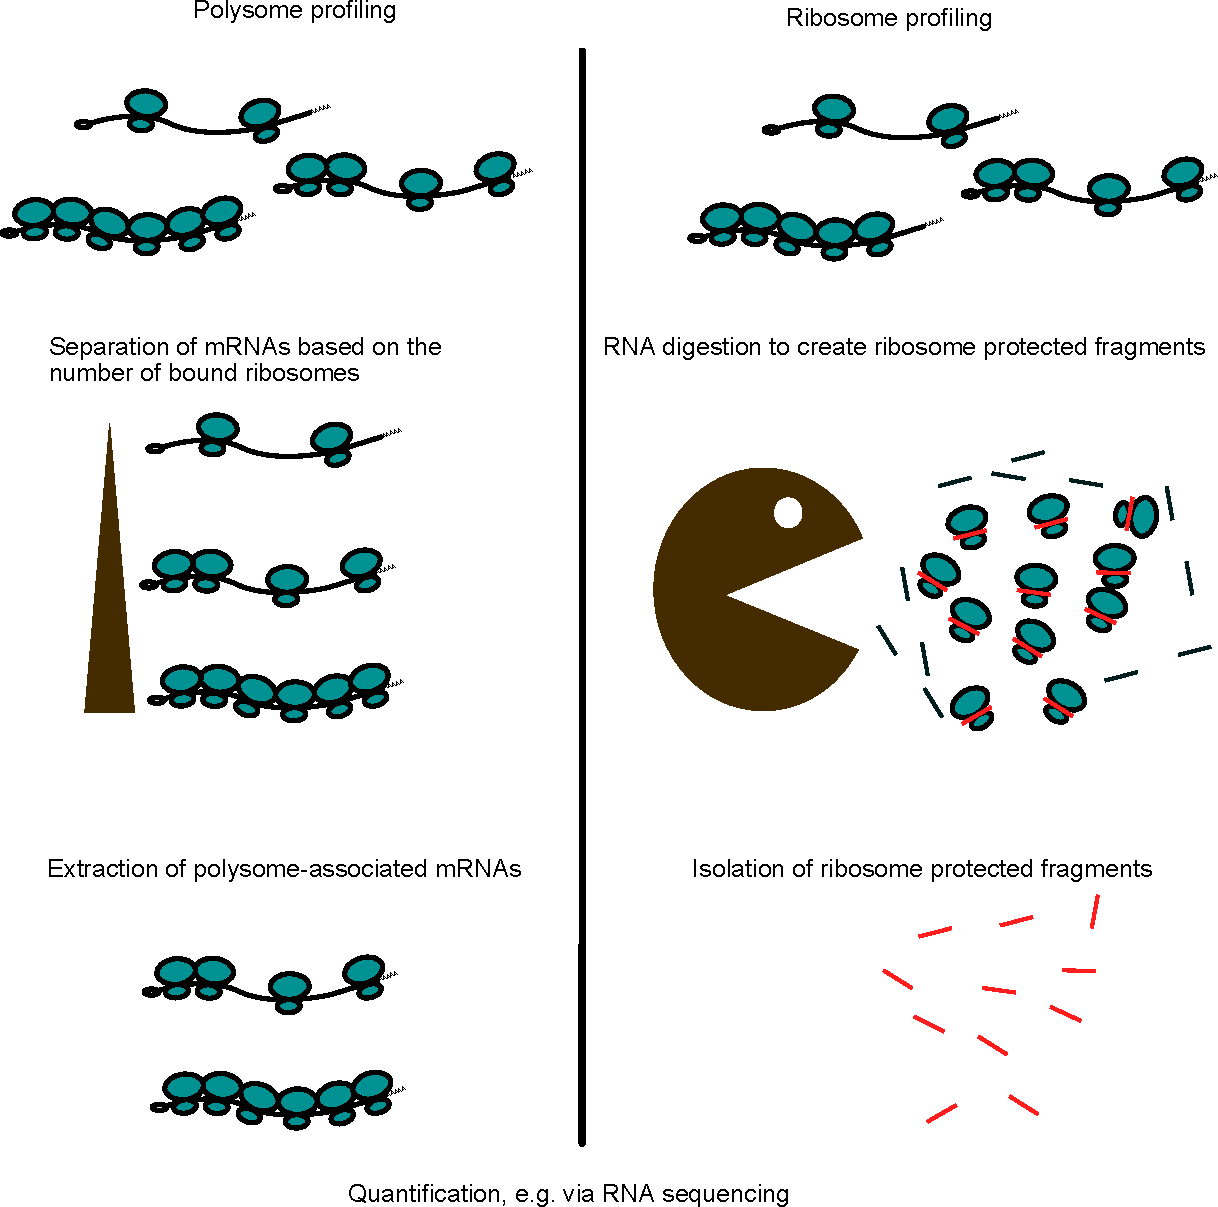
\includegraphics{./figures/polyRibo.pdf}
  \caption{Polysome profiling and ribosome profiling workflows. In polysome profiling a fraction from whole cytoplasmic RNA is loaded onto a sucrose gradient on which they get separated by sedimentation into the sucrose gradient using ultra centrifugation. Fractions corresponding to efficiently translated mRNAs are collected and can be quantified with for example RNA sequencing (left). During ribosome profiling a fraction from the whole cytoplasmic RNA is exposed to a digestion agent which breaks the RNA. Ribosomes will protect fragments thereby creating ribosome protected fragments. These fragments are then isolated and can be sequenced. Note the differently coloured mRNAs and how both methods separate them. \label{fig:polyRibo}}
\end{wrapfigure}

Two methods are predominantly used for measuring mRNA translation to estimate changes in translation efficiencies across conditions, namely polysome profiling and ribosome profiling (\textbf{see figure \ref{fig:polyRibo}}). These methods capture the number of ribosomes an mRNA is associated with. The number of bound ribosomes is an adequate of estimator changes in translation efficiencies when initiation is rate limiting. Indeed, as explained above this is a common scenario (\emph{see section \ref{transEff}}).

\subsection{Polysome profiling}

Polysome profiling allows for separation of polysomes from monosomes, ribosomal subunits and messenger ribonucleoprotein particles (mRNPs). During this assay, ribosomes are immobilized on the mRNAs using translation elongation inhibitors, e.g.~cycloheximide (CHX). Cytoplasmic extracts sediment on a linear sucrose gradient (5-50\%) using ultra centrifugation. The resulting gradient is fractionated and mRNAs with different numbers of bound ribosomes can be extracted and analyzed for mRNA content (Gandin et al., 2014). Typically fractions belonging to mRNAs with more than 3 bound ribosomes are pooled. A 3-ribosome cutoff has been chosen as it is thought to capture most biologically relevant changes in translation efficiency (Gandin, Masvidal, Hulea, et al., 2016).

\begin{wrapfigure}{r}{0.6\textwidth}
    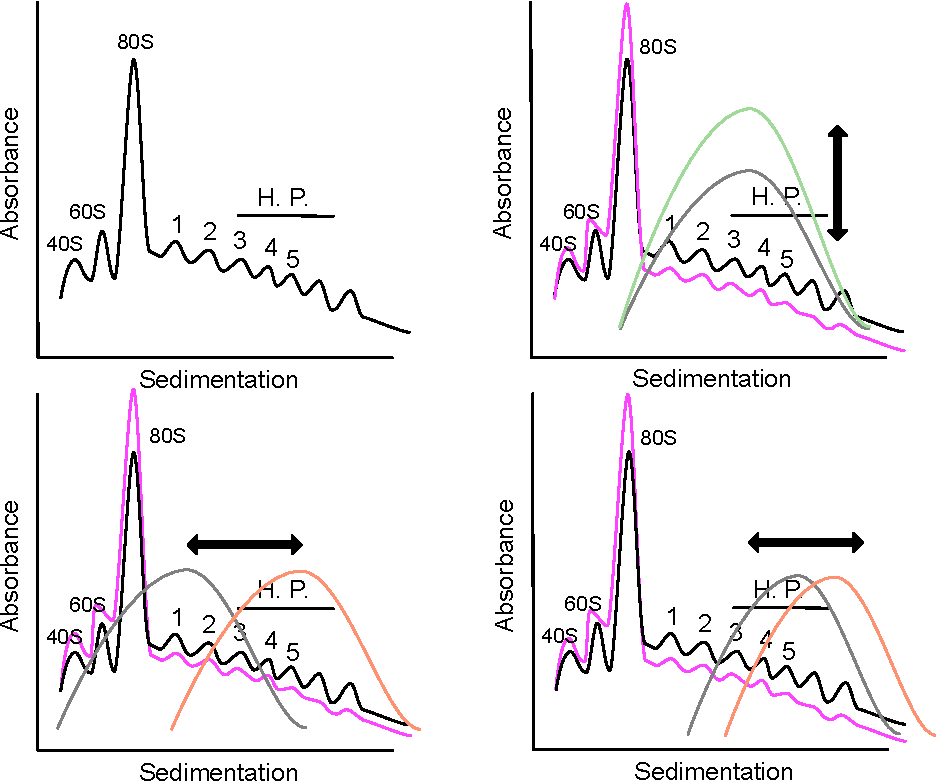
\includegraphics[width=0.9\linewidth]{./figures/polysome_shifts.pdf}
  \caption{Polysome profliles -  (top left) Schematic representation of a polysome profile using linear sucrose gradient fractionation. Indicated in the polysome profiles are the 40S, 60S ribosomal subunits as well as the 80S monosome. H.P. indicates heavy polysome fractions. Between conditions (i.e. black an pink lines) distribution changes for mRNA abundance (grey and green; top right), translation (grey and red; bottom left) and translation within high polysome fractions (grey and red; bottom right) are illustrated. \label{fig:polysome}}
\end{wrapfigure}

An illustration of a polysome profile with peaks for the 40S, 60S subunits and 80S ribosome can be seen in (\emph{Fig \ref{fig:polysome} top left}). Subsequent peaks along the fractions indicate the mRNAs with 2 or more bound ribosomes. mRNAs are typically normally distributed along the fractions, i.e.~in a pool of the same mRNA many will be associated with different numbers of ribosomes (Gandin, Masvidal, Hulea, et al., 2016). Changes in mRNA abundance may lead to an overall increase in the amount of isolated polysome-associated mRNA without a shift of the distribution along the fractions (\emph{Fig \ref{fig:polysome} top right}). This means that the translation efficiency per mRNA remains unchanged. In contrast, changes in translational efficiency can be observed by shifts along the polysome fractions. For example, if the mRNAs shift from the light (inefficiently translated) towards the heavy (efficiently translated) polysome fractions or vice versa in the absence of changes in total mRNA levels (\emph{Fig \ref{fig:polysome} bottom left}). Shifts within the heavy polysome fractions (i.e.~with a mean distribution around 4 bound ribosomes to 7 bound ribosomes) can also occur (\emph{Fig \ref{fig:polysome} bottom right}). Quantification of mRNA levels within each fraction can be assessed using Northern blotting or reverse transcription quantitative polymerase chain reaction (RT-qPCR). For transcriptome-wide studies, efficiently translated mRNAs are pooled and quantified using either DNA-microarrays or RNA sequencing.

Pooling of mRNAs as well as collection of multiple fractions makes polysome profiling inconvenient when dealing with low amounts of input RNA or with large samples sizes. Therefore, an optimised sucrose gradient was developed where mRNAs bound to \textgreater3 ribosomes are collected on a sucrose cushion and thereby can be isolated from one single fraction (Liang et al., 2018). This optimised gradient allows for application of polysome profiling in small tissue samples where RNA quantity is limiting and reduces labour intensity of the assay.

Polysome-associated mRNA levels are subject to changes in translation efficiency as well as factors contributing to cytosolic mRNA levels. Cytosolic mRNA levels impact the pool of mRNAs that can associate with ribosomes. However, changes in cytosolic can occur due to, e.g.~transcription or mRNA stability. Therefore, to identify true changes in translation efficiency it is important to collect cytoplasmic mRNA and polysome-associated mRNA from the same sample in parallel to correct for such mechanisms during downstream analysis.

\subsection{Ribosome profiling} \label{riboseq}

R17 bacteriophage ribosome protected RNA fragments (RPFs) have been obtained in the 1960s using ribonucleosases to trim away mRNA sequences not protected by ribosomes (Steitz, 1969). More recently ribosome profiling has been developed. Ribosome profiling encompasses sequencing of RPFs on a transcriptome-wide scale (Ingolia et al., 2009; Ingolia, 2016). Similar to polysome profiling, in the ribosome profiling assay ribosomes are immobilised on mRNAs using translation elongations inhibitors (e.g.~CHX).

RPFs are obtained by RNAse treatment that degrades the links of RNA between ribosomes leaving single ribosomes covering a \textasciitilde28 nucleotide long RNA fragment. However, as ribosomal RNAs (rRNA) are also degraded during this process they represent a major contaminant herein. The RPFs are then isolated using ultra centrifugation through a sucrose cushion. During this step other RNA fragments such as rRNAs, non-coding RNAs (ncRNAs) or large ribonucleoprotein complexes can co-migrate and contaminate the sample. Typically, RPFs with a size ranging from 25-30 nucleotides are selected for quantification. However, RBP-or 43S-protected RNAs, such as those localised in stress granules, may produce fragments of similar length. Furthermore, ribosomes undergoing conformational changes have been shown to protect fragments corresponding to a length of 21nt when translation elongation is blocked by e.g., CHX (Lareau et al., 2014). Therefore, size selection can distort the estimation of translation efficiency from ribosome profiling data (Dmitry E. Andreev et al., 2017). From the resulting RPFs libraries are generated and quantified using RNA sequencing. During library construction additional biases due to enzyme sequence preferences can be introduced that can lead erroneous estimations of codon positions within the ribosome (Artieri et al., 2014a).

Recently, the algorithm Ribo-seq Unit Step Transformation (RUST) has been developed (O'Connor et al., 2016). RUST can reveal mRNA sequence features affecting RPF density globally. The authors applied RUST to 30 publicly available data sets and identified substantial sequence heterogeneity affecting RPF densities. Thus, sequence bias is prominent in ribosome profiling (O'Connor et al., 2016).

Initially, fragmented total mRNA using alkaline hydrolysis of the same size were retrieved in parallel to RPFs. This was achieved by extraction of total mRNA from cell lysate followed by purification via recovery of polyadenylated messages or removal of ribosomal RNA (Brar et al., 2015; Ingolia et al., 2009). The random fragmentation of total mRNA has been shown to result in experimental bias. Therefore, now sequencing of unfragmented total mRNA in parallel is preferred.

\subsection{Comparing ribosome and polysome profiling}

Albeit both methods generate count data after quantification with RNA sequencing, there are some key aspects that differ between the techniques. Polysome profiling separates efficiently translated mRNAs from non- efficiently translated mRNAs along a sucrose gradient thereby creating an mRNA-based perspective for analysing changes in translational efficiencies. In contrast, ribosome profiling determines translational efficiencies by counting the number of RPFs of both efficiently and non-efficiently translated mRNAs (\emph{see figure \ref{fig:polyRibo}}). This can have implications for identification of transcript variants. For example, if a ribosome would not protect a fragment differentiating two isoforms, information on the isoforms would be lost during ribosome profiling (Floor et al., 2016). In polysome profiling the integrity of the mRNA is preserved. This gives polysome profiling the advantage in cases where transcript variants with different 5' UTR lengths are of interest. This makes polysome profiling, but not ribosome profiling, compatible with methods to investigate UTRs (e.g.~CAGE and 3P-seq) (Jan et al., 2011; Takahashi et al., 2012).

Shifts in ribosome association can be dramatic (e.g.~near complete dissociation of ribosomes from an mRNA) or subtle (e.g.~shifts from 2 to 4 ribosomes). These shifts can occur due to different properties of the mRNAs the ribosomes associate with (Gandin, Masvidal, Hulea, et al., 2016). When dramatic and subtle changes in ribosome association are present in parallel, ribosome profiling is biased towards identification of shifts with a greater magnitude and masks the subtle ones (Gandin, Masvidal, Hulea, et al., 2016). Gandin et. al.~showed under mTOR inhibition ribosome profiling studies are likely to predominantly identify TOP mRNAs (i.e.~heavy shifters). In contrast, polysome profiling identified both TOP and non-TOP mRNAs (i.e.~more subtle shifters compared to TOP mRNAs) when mTOR is inhibited (Gandin, Masvidal, Hulea, et al., 2016). Therefore, in scenarios where global mRNA translation is affected, application of ribosome profiling could lead to imprecise biological conclusions. The masking of subtle changes has been attributed to the indirect estimation of translation efficiencies from counting RPFs for ribosome profiling, which is highly dependent on the abundance of mRNAs. In polysome profiling this effect is much less pronounced as changes in translation efficiency are directly estimated from the mRNAs associated with heavy polysomes (Masvidal et al., 2017). Therefore, polysome profiling is more suitable than ribosome profiling in studies that aim to analyse global changes in translation efficiences. (Gandin, Masvidal, Hulea, et al., 2016; Masvidal et al., 2017).

An advantage of ribosome profiling is that it provides exact nucleotide positions occupied by ribosomes. This offers information at a single nucleotide level where the ribosome is located at the mRNA. Polysome profiling cannot reveal ribosome locations along the mRNA. The single nucleotide resolution of ribosome profiling is necessary in contexts studying events such as ribosomal frame shifts or uORF translation (Dmitry E. Andreev et al., 2015; Rato et al., 2011). One limitation of ribosome profiling to identify features such as uORFs, is the use of elongation inhibitors (e.g.~CHX) as pre-treatment in the protocol. After CHX treatment elongation is not immediately inhibited but continues for several cycles (Hussmann et al., 2015). Studies investigating stress in yeast showed that increases in ribosome occupancy were due to CHX treatment rather than stress (Gerashchenko et al., 2014). Therefore, CHX pre-treatment can introduce biases in ribosome profiling obscuring identification of sequence features that are potentially important for translational regulation (Gerashchenko et al., 2014; Hussmann et al., 2015).

Both methods have their strengths and weaknesses. Thus, when designing an experiment each method should be considered and chosen depending on the underlying biological question.
\newline

\section{Modes for regulation of gene expression through mRNA translation} \label{modes}
\begin{wrapfigure}{r}{0.6\textwidth}
  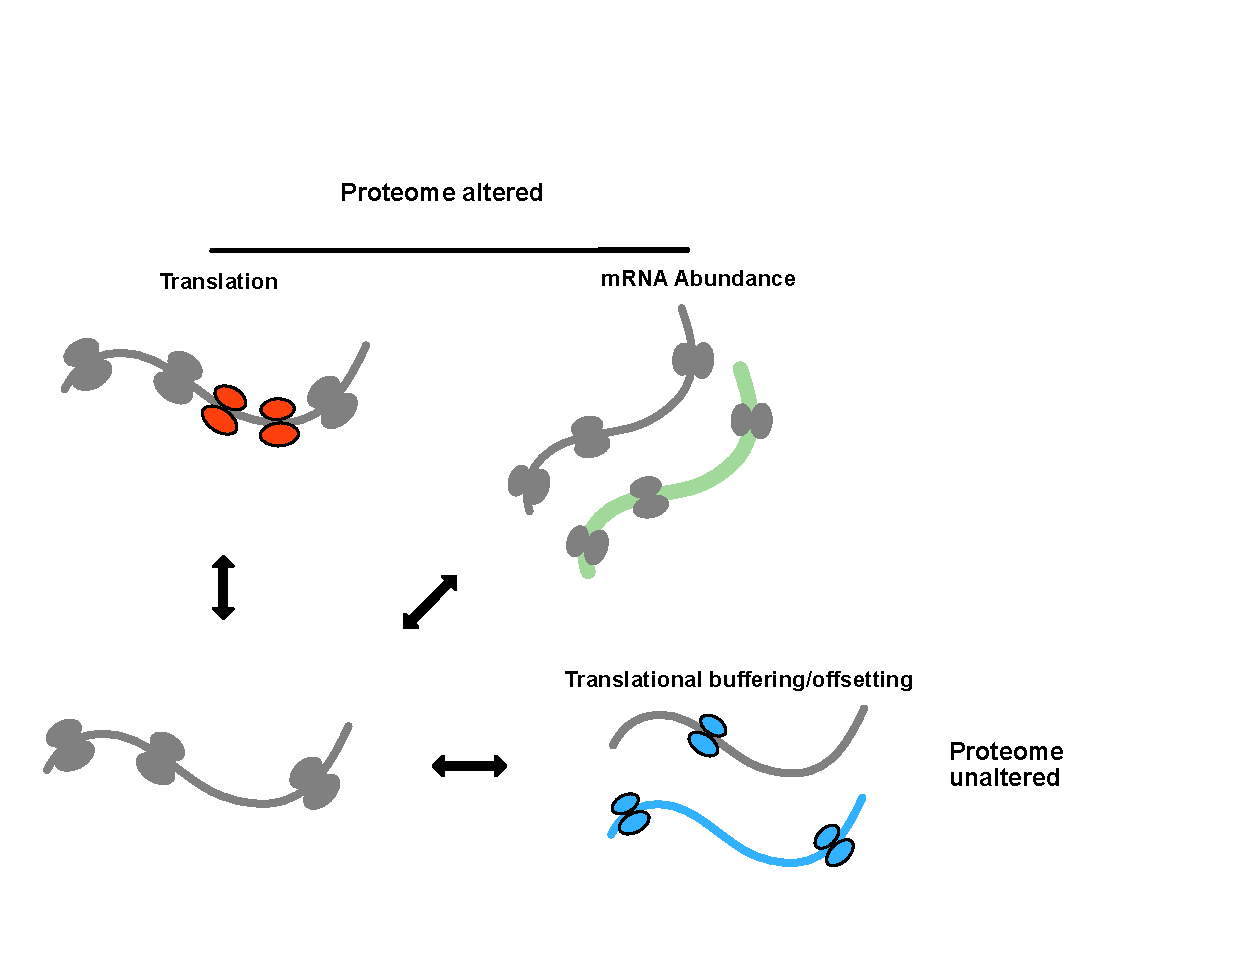
\includegraphics{./figures/geneModes_MRNA.pdf}
  \caption{Modes for regulation of gene expression - Schematic representation of modes by which mRNA translation regulates gene expression. Indicated are: changes of the translation mode, i.e. an mRNA increases its ribosome association without a change in total mRNA levels; The mRNA abundance mode, i.e. changes in total mRNA levels paralleled by changes in translated mRNA levels; The translational buffering mode, i.e. changes in total mRNA levels without changes in translated mRNA levels. Also indicated is the expected outcome on the proteome for all three modes. \label{fig:modes}}
\end{wrapfigure}

From transcriptome-wide assessments of translation using ribosome or polysome profiling expression levels for both cytoplasmic and polysome-associated mRNAs (or RPFs) are obtained. For simplicity, from now on, these RNA types will be referred to as total mRNA (i.e.~cytoplasmic mRNA) and translated mRNA (i.e.~polysome-associated mRNA or RPFs). The estimation of expression levels for both translated mRNA and total mRNA allows distinction between changes occurring at total mRNA level or translation and their integration. This is important because, the interplay of total mRNA with translated mRNA can give valuable insights about the underlying mechanisms that govern gene expression in the studied system.

When comparing perturbed systems to their corresponding control state three ``modes'' in which translated mRNA and total mRNA distinctly interact can be observed (\emph{see figure \ref{fig:modes}}). These modes are referred to as ``mRNA abundance,'' ``translation'' (i.e.~changes in translation efficiencies leading to altered protein levels) and, ``translational buffering'' (i.e.~changes in translation efficiencies ensuring stable protein levels across conditions).

\subsection{mRNA Abundance mode}

A change in mRNA abundance is observed when total mRNA levels change, by e.g.~transcription or mRNA stability, but the translation efficiency of those mRNA is unaltered. (\emph{see figure \ref{fig:modes}}). The change in total mRNA levels alters the number of mRNAs to compete for components of the translation machinery. Thus, their association to ribosomes can be explained by their abundance. While the translation efficiency for these mRNAs is unaltered, a modulation of protein synthesis is expected as more or less mRNAs are translated.

\subsection{Translation mode}

A change in translation occurs when translated mRNA levels either increase or decrease, while corresponding total mRNA levels remain constant or change to a lesser extent (\emph{see figure \ref{fig:modes}}). The change in ribosome association independent of total mRNA levels is therefore a change in their translation efficiency. A prominent example of this mode can be observed for TOP mRNAs. Under conditions when mTOR is inhibited, TOP mRNAs show a near complete disassociation from ribosomes (Gandin, Masvidal, Hulea, et al., 2016). Furthermore, during the ISR, translation of ATF4 mRNA is altered due to eIF2\(\alpha\) phosphorylation. Similar to changes in mRNA abundance, mRNAs under the translation mode lead to changes in corresponding protein levels (\emph{see figure \ref{fig:modes}}).

\subsection{Translational buffering mode} \label{modeBuffering}

The third mode of regulation of gene expression is termed translational buffering. Under this mode, a change in total mRNA levels is observed, whereas polysome-associated mRNA levels remain constant between conditions. Translational buffering thus reflects a change in translation efficiency as the proportion of mRNAs associated with ribosomes is altered. In contrast to changes in translation and mRNA abundance, translational buffering has been shown to maintain similar protein levels across conditions rather than inducing alterations to them (\emph{See figure \ref{fig:modes}}) (Lorent et al., 2019; McManus et al., 2014).

Current literature supports multiple forms of translational buffering. Translational buffering can compensate for differences in mRNA levels due to e.g.~differences in gene dosages, so that protein levels remain similar (Dassi et al., 2015; Lalanne et al., 2018). Furthermore, rather than compensating it can ``offset'' modulations of total mRNA levels at the level of translation to maintain corresponding protein levels (Lorent et al., 2019).

Translational buffering in its compensation form has been observed at steady state levels. A study comparing co-evolution of transcription and translation across seven different organs and mammals showed overall greater divergence of transcription as compared to translation (Z.-Y. Wang et al., 2020). Similar compensation at the level of translation has been observed between individuals, tissues and prokaryotes (Artieri et al., 2014b; Cenik et al., 2015; Dassi et al., 2015; Lalanne et al., 2018; Perl et al., 2017).

Compensation via translational buffering can also enforce equilibration of pathway or protein complex stoichiometry (Lalanne et al., 2018; G.-W. Li et al., 2014). An example of this was observed in evolutionary distant bacteria, i.e.~\emph{B. subtilis} and \emph{E. coli}. In \emph{B. subtilis} translation related factors rpsP and rplS are located in different operons, whereas in \emph{E. coli} rpsP and rplS lie within the same operon as rimM and trmD. While \emph{B. subtilis} can fine tune transcription at the different operons, in \emph{E. coli} these will be transcribed together. However, in \emph{E. coli} rimM and trmD are only required in low protein abundance, whereas rpsP and rplS are required in high abundance. \emph{E. coli} compensates the transcriptional input at the translational level and thus equilibrates for requirements in pathway stoichiometry (Lalanne et al., 2018).

As mentioned above, a different form of translational buffering can be observed in perturbed systems that offset changes in total mRNA levels at the level of translation temporarily. For example, translational offsetting was observed in prostate cancer cells where a transcriptional program was induced under estrogen receptor \(\alpha\) (ER\(\alpha\)) depletion that showed no increase in polysome-associated mRNA. mRNAs whose transcription was translationally offset required the tRNA U34 modification. ER\(\alpha\) has been shown to regulate the expression of the catalytic enzymes required for the U34 modification (Lorent et al., 2019). Thus, depletion of ER\(\alpha\) led to impeded modification of tRNAs at the U34 position. Therefore, the translation efficiency of mRNAs requiring the modification was reduced despite increased total mRNA levels. The authors confirmed that protein levels of translationally offset mRNAs were unaltered between conditions (Lorent et al., 2019).
\newline

\section{Algorithms for analysis of changes in translation efficiencies}\label{algorithm}

As discussed above, the proteome can be reshaped via multiple modes for regulation of gene expression. Furthermore, these modes can have different underlying mechanisms. It is therefore warranted to distinguish them in analysis of translation efficiencies. This section discusses methods to analyse polysome-profiling and ribosome profiling data to estimate changes in translation efficiencies across 2 or more conditions.

Initially, analysis of transcriptome-wide translation studies used an approach called the translation efficiency score (TE-score) that applied the following equation:
\[\varDelta TE = \frac{\frac{P_{c2}}{T_{c2}}} {\frac{P_{c1}}{T_{c1}}}\\\]

This score calculates the ratio of the ratios between polysome-associated mRNA levels (P) divided by total mRNA levels (T) within each condition, i.e.~C1 and C2. The TE- score approach has been shown to be prone to spurious correlations (Larsson et al., 2010). Spurious correlations arise due to that the ratio of polysome-associated mRNA and total mRNA can systematically correlate with total mRNA levels which is not corrected for in this equation and leads to an elevated type-1 error.

\emph{Figure \ref{fig:TE}} gives an overview of the relationship between a change in TE-score and each gene expression mode (\emph{see also figure \ref{fig:modes}}). Changes in mRNA abundance will lead to a \(\varDelta\)TE close to 0 in log space (i.e.~no change in translation efficiency). This is due to that total mRNA and translated mRNA change with a similar magnitude. However, in the case of both the translation mode and the translational buffering mode, the nominator and denominator in the TE-score equation change leading to a \(\varDelta\)TE (TE \textless{} 0 or TE \textgreater{} 0). Therefore, the TE-score cannot distinguish between changes belonging to the translation mode from changes of the translational buffering mode. This can have drastic consequences for the interpretation of the results.
\clearpage

\begin{wrapfigure}{o}{0.5\textwidth}
  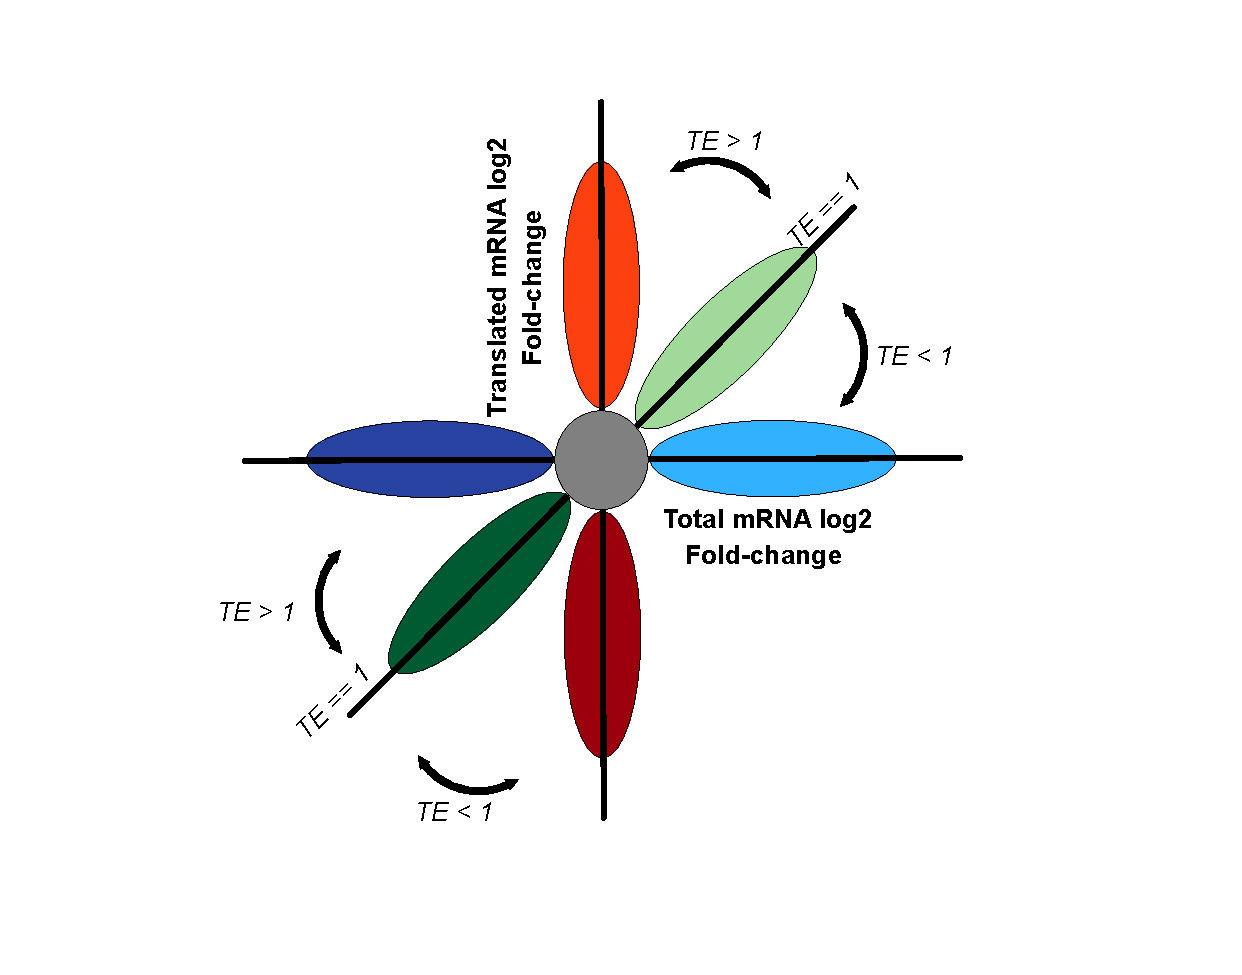
\includegraphics{./figures/geneModes_TE.pdf}
  \caption{TE-scores for modes for regulation of gene expression -  Schematic representation of modes for regulation of gene expression in a fold-change scatter plot. The x-axis indicates the fold-change for total mRNA levels. The y-axis indicates the fold-change for translated mRNA levels. Indicated in red are changes in translation efficiency altering protein levels (i.e. translation mode), in green changes in mRNA abundance and in blue changes in translation efficiency leading to translational buffering/offsetting. The relationship for the TE-score and the modes for regulation of gene expression is indicated. \label{fig:TE}}
\end{wrapfigure}

The TE-score approach was questioned when proposing the Analysis of Translation Activity (anota) algorithm which was developed for DNA-microarray data (Larsson et al., 2010). Anota combines analysis of partial variance (APV) (Schleifer et al., 1993) with a random variance model (RVM) (Wright et al., 2003). RVM estimates gene variance using shared information across all genes to increase power for detection of differential expression (Wright et al., 2003). Anota uses a two-step process that firstly assesses the model assumptions for (i) absence of highly influential data points, (ii) samples classes sharing a common slope, (iii) homoscedasticity of residuals and (iv) normal distribution of per gene residuals. In the second step anota performs analysis of changes in translational activity using the following model:

\[y_{gi} = \beta_g^{RNA}\ X_i^{RNA}+ \beta_g^{cond}\ X_i^{cond} + \varepsilon_{gi}\]

here \(y_{gi}\) is the polysome associated mRNA expression, \(\beta_g^{RNA}\) describes the relationship to total RNA for the \(gth\) gene of the \(ith\) sample column of model matrix \(X\); \(\beta_g^{cond}\) represent the difference in intercept between treatment classes and \(\varepsilon_{gi}\) denotes the residual error.
\clearpage

\begin{wrapfigure}{o}{0.5\textwidth}
  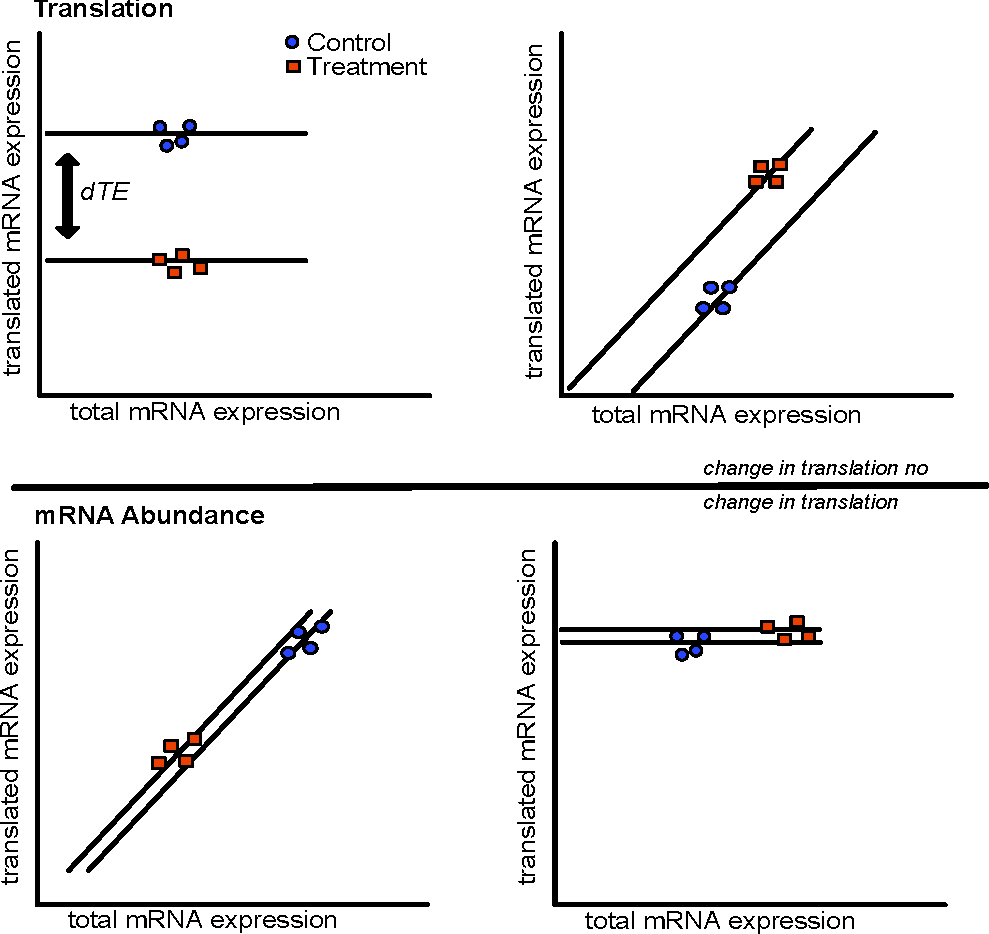
\includegraphics{./figures/geneModes_anota_Larsson.pdf}
  \caption{anota gene models - Schematic representation of the anota analysis models. Translated mRNA expression is set out against total mRNA expression for each biological replicate and treatment condition. Top left shows the model of a gene that is differentially translated (i.e. change in translated but not total mRNA). The difference in the slope intercepts is used to estimate changes in translation efficiencies between conditions. Other gene models are shown; change in translation efficiency leading to altered protein levels with varying total mRNA levels (top right); change in mRNA abundance (bottom left) and translational buffering (bottom right).
  \label{fig:anota}}
\end{wrapfigure}

Within anota, a common slope for the treatment classes that describes the relationship between translated mRNA and total mRNA is calculated. The difference between the slope intercepts is then interpreted as the change in translation efficiency. A simplified view of this model is provided in (\emph{Figure \ref{fig:anota} top left}). Here, expression for translated mRNA and total mRNA are modeled over two sample classes that each has 4 replicates. Changes in translation efficiencies can also be observed when translated mRNA expression is modulated to a larger extent than the total mRNA levels (\emph{Figure \ref{fig:anota} top right}). Identification of genes in this category can be a challenge, especially in highly variable data sets, as they resemble genes regulated at the level of mRNA abundance (\emph{Figure \ref{fig:anota} bottom left}). Nevertheless, using the linear regression analysis anota accurately corrects changes in translated mRNA as can be seen in (\emph{Figure \ref{fig:anota} bottom right}). Here, a change in total mRNA but not translated mRNA levels is observed. For this gene, the difference in slope intercepts between sample classes is small and will not be identified as differentially translated as would be the case in the TE-score approach. Anota was developed at a time where translational buffering was not considered in data sets. Naturally, the method lacks a setting to analyse translational buffering. This was addressed in anota's successor, anota2seq, and will be discussed in \emph{Study 1}.

Advances in experimental methods warrant for appropriate statistical approaches to analyse data resulting from them. DNA-microarray was the dominant platform to assess transcriptome-wide changes before the advent of RNA sequencing. DNA-microarrays measure intensity after hybridisation events which is an indicator of expression. In contrast, in RNA sequencing reads of constructed libraries are counted. Intensity data from DNA-microarray can be normalised and transformed (i.e.~log transformation) to fulfill the requirements for application of linear models, whereas RNA sequencing harbours additional characteristics that need to be accounted for. Therefore, algorithms developed for analysis of DNA- microarray are not directly applicable to RNA sequencing data as is the case for the anota algorithm.

RNA sequencing data shows variance that is greater than the mean which is commonly referred to as overdispersion. Count data from RNA sequencing have been initially approached using Poisson distributions which assumes that the variance is equal to the mean (Lu et al., 2005). Now established RNA sequencing analysis frameworks such as edgeR and DESeq2 use negative binomial distributions in combination with generalised linear models (GLMs) (Love et al., 2014; Robinson et al., 2010). The negative binomial distribution uses a dispersion parameter to account for differences in the mean-variance relationship across the expression range (McCarthy et al., 2012). While analysis principles of DESeq2 and edgeR are similar, they differ in their normalisation method, dispersion estimation and information sharing across genes. In a simple differential expression analysis between two conditions with one RNA type the GLM model would be as in the following equation:

\[log(y_{gi}) = \beta_g^{cond}\ X_i^{cond} + \varepsilon_{gi}\]

here \(\beta_g^{cond}\ X_i^{cond}\) represent the condition (i.e.~control and treatment) log2 fold change for the \(gth\) gene \(ith\) sample column of the model matrix X and \(\varepsilon_{gi}\) denotes the residual error. When analysing changes in translation effiencies additional parameters for RNA type (i.e.~total mRNA or translated mRNA) and the interaction between the RNA type and condition are added so that:

\[log(y_{gi}) = \beta_g^{RNA}\ X_i^{RNA}+ \beta_g^{cond}\ X_i^{cond} + \beta_g^{RNA:cond}\ X_i^{interaction} + \varepsilon_gi\]

In this model, the interaction term is interpreted as the change in translation effiencies (Chothani et al., 2019). Other methods (i.e.~Ribodiff (Zhong et al., 2017), Riborex (W. Li et al., 2017) and deltaTE (Chothani et al., 2019)) borrow this analysis principle of an GLM with an interaction term by applying this exact model. A notable difference is that Ribodiff allows dispersion estimation for translated mRNA and total mRNA separately. Differences in within-RNA variances between RNA types can be expected due to varying experimental protocols (Liang et al., 2018; Zhong et al., 2017). While the flexibility of GLMs allows for complex study designs involving 2 or more treatment conditions, Riborex and Ribodiff limit the study design to only two conditions. DeltaTE gives their users full flexibility of the DESeq2 GLM model. Xtail is a method developed for ribosome profiling that makes use of DESeq2 for RNAseq count normalisation (Z. Xiao et al., 2016). Their assessment of differences in translation efficiencies relies on probability matrices for the ratio of translated mRNA over total mRNA within condition and a between condition ratio of these ratios. Babel was the first algorithm designed solely for analysis of differential translation and uses an error-in-variables regression analysis (Olshen et al., 2013). The error-in-variables regression allows accounting for variable total mRNA levels when assessing changes in translation. Although these methods have distinct approaches to identify changes in translation efficiencies, their principle of analysis is similar to comparing a ratio of ratios (see TE-score equation above). Therefore, these methods suffer from similar issues as the TE-score which will be discussed in \textbf{Study 1}.

\chapter{Aims of this thesis}

This thesis aims to expand current methodologies for analysis of translation efficiency data and explore the regulation of gene expression in cancer.

In \textbf{Study I}, we adapted the ANalysis Of Translation Activity data (anota) algorithm so that it could be applied to next-generation sequencing data. Furthermore, we implemented the analysis of translational buffering a recently described mode for regulation of gene expression. The resulting algorithm was named anota2seq.

We then applied the anota2seq algorithm to investigate changes in translation efficiencies in two cancer models:

In \textbf{Study II} we unravelled the effects of eIF4A, an RNA helicase, inhibition using a synthetic rocaglate CR-1-31-B (CR-31) in pancreatic ductal adenocarcinoma.

In \textbf{Study III} we explored the effects of insulin on gene expression in multiple cell lines.

\chapter{Results and discussion}

\section{Study 1 - Generally applicable transcriptome-wide analysis of translation using anota2seq}

Initially, changes in translation efficiencies were estimated using the TE-score approach as outlined in section \ref{algorithm}. However, this method was shown to be prone to spurious correlations. This leads to elevated false positive identification that can result in erroneous biological conclusions (Larsson et al., 2010). When using the TE-score, spurious correlations can be attributed to the inadequate correction for changes in total mRNA levels when estimating translation efficiencies (Larsson et al., 2010, 2011). The Analysis of Translation Activity (anota) algorithm facilitates analysis of translational efficiencies that are corrected for changes in total mRNA levels (Larsson et al., 2011).

Anota was developed for analysis of transcriptome-wide analysis for data quantified by DNA- microarrays (Larsson et al., 2010). However, advances in experimental methodologies lead to the development of RNA sequencing. RNA sequencing and DNA microarray data have distinct characteristics that need to be accounted for before analysis (\textbf{see section \ref{algorithm}}). Therefore, while the statistical framework of anota was shown as an adequate approach for analysis of translational efficiencies DNA microarray data, it was not directly applicable to RNA sequencing data (\emph{see section \ref{algorithm}}). Efforts have been made to make RNA sequencing data more ``DNA-microarray-like'' so that algorithms developed for intensity based microarray data can be applied to count based RNA sequencing data (Law et al., 2014; Love et al., 2014). Anota2seq, the algorithm developed in this study, allows for transformation and normalisation of RNA sequencing data so that the anota statistical framework can be applied for analysis of count data.

Another feature of anota2seq is that it allows for statistical analysis of translational buffering. The need for the analysis of translational buffering, or the uncoupling of total mRNA levels from translation, has been noted before anota2seq's development by comparing 20 translatomes and transcriptomes with different underlying stimuli in mammalian cells (Tebaldi et al., 2012). The same authors proposed a framework, called tRanslatome, that combines several methodologies for analysis of differential transcription and translation efficiencies, including anota, for a comprehensive analysis of transcription and translation as well as their underlying mechanisms (Tebaldi et al., 2014).

\begin{wrapfigure}{o}{0.5\textwidth}
  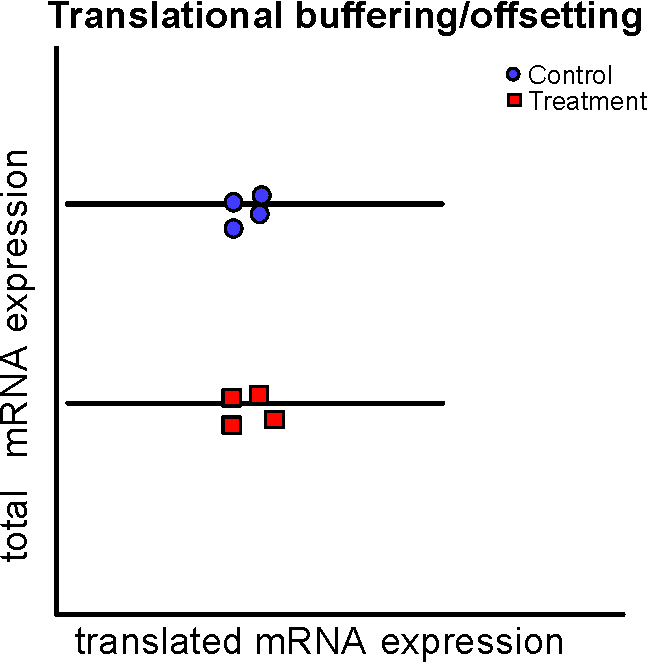
\includegraphics{./figures/geneModes_anota2seq.pdf}
  \caption{anota2seq gene model for analysis of translational buffering /offsetting - Total mRNA expression is set out against translated mRNA expression for each biological replicate and treatment condition. The model shows total mRNA changes that are independent of translated mRNA changes, i.e. translational buffering (see section \ref{modes}).
  \label{fig:anota2seq}}
\end{wrapfigure}

Nevertheless, commonly observed in polysome and ribosome profiling data sets are three gene expression modes, translation, translational buffering and mRNA abundance. While anota can be used to identify genes among the translation and mRNA abundance modes, analysis of translational buffering was not implemented therein (\emph{See Figure \ref{fig:anota}}). Therefore, one would need to rely on the integration of several methods to efficiently analyse transcriptome-wide studies of translation efficiencies. Anota2seq addresses this issue by changing the analysis model as described in section \ref{algorithm} to analyse changes in total mRNA levels corrected for changes in translated mRNA levels (i.e.~translational buffering, \emph{see figure \ref{fig:anota2seq}}).

Application of anota2seq has successfully identified translational buffering to which biological mechanisms could be linked (Lorent et al., 2019). Furthermore, in \textbf{study 2} translational buffering can be observed as a compensating mechanism in ``healthy'' cells upon treatment with an eIF4A inhibitor and in \textbf{study 3} we identify mTOR dependent translational buffering for mRNAs with certain 3' UTR characteristics.

The aim of this study was to compare anota2seq's performance to other established algorithms (i.e.~DESeq2, RiboDiff, babel, TE-score and Xtail) for analysis of translation efficiencies. More specifically, we were interested in their ability to distinguish the three prominent modes of gene expression (\emph{see figure \ref{fig:modes}}). To achieve this we used simulated data. While it is arguable to what extent conclusion drawn from simulated data can be extended towards empirical data, it allows for a controlled environment where true positive changes are known in advance. The mean-variance relationship in the simulated data is based on a real polysome profiling data set to increase confidence that drawn conclusions are also applicable to empirical data (Guan et al., 2017). Furthermore, during testing of our simulation we used an additional data set to estimate parameters from to generate data sets. Using these simulated data to compare the performance of the above mentioned algorithms showed almost identical results.

The simulated data consisted of four replicates for translated mRNA and total mRNA with a ``control'' and a ``treatment'' condition. The data sets also contained a combination of the following gene sets:

\emph{Unchanged}: For this simulation category we sampled reads from the same NB distribution for both the control and treatment conditions in both the translated and total mRNA. This category represents genes that would be unaffected by e.g.~a stimulus.

\emph{mRNA abundance}: For this category the control condition for both the translated mRNA and total mRNA were sampled from the same NB distribution. The NB distribution for \textbf{both translated mRNA and total mRNA} of the treatment condition was altered so that values would be drawn corresponding to a fold change (negative or positive) ranging between 1.5 to 3.0. The directionality of the fold changes (i.e.~up or down regulation) was the same for translated mRNA and total mRNA.

\emph{translation}: For this category the control condition for both the translated mRNA and total mRNA were sampled from the same NB distribution. The NB distribution for \textbf{translated mRNA only} of the treatment condition was altered so that values would be drawn corresponding to a fold change (negative or positive) ranging between 1.5 to 3.0.

\emph{buffering}: For this category the control condition for both the translated mRNA and total mRNA were sampled from the same NB distribution. The NB distribution for \textbf{total mRNA only} of the treatment condition was altered so that values would be drawn corresponding to a fold change (negative or positive) ranging between 1.5 to 3.0.

As a first step, we tested whether the methods could properly control for type-1 errors (i.e.~false positive identification). For this we simulated a data set with genes belonging only to the ``unchanged'' category. This revealed that babel, but to an even greater extent Xtail, were unable to control their type-1 error as these methods assigned low p-values and FDRs when no real changes were present. DESeq2 was marginally affected by this also. This indicated a limited applicability of Xtail and babel for statistical analysis of translatomes.

From the comparative analysis of the analysis for changes in translation efficiencies affecting protein levels we concluded that anota2seq outperforms all other methods. This was assessed by comparing the area under the curve from Receiver operating characteristics (ROC) and precision recall curves. The ROC curves showed a, albeit slightly, better performance for detecting changes in translation. However, the precision recall was much higher for anota2seq. This can be accredited to that the analysis principle of the other methods is similar to the TE-score (\emph{as explained in section \ref{algorithm}}). Nevertheless, when comparing the performance using simulated data in the absence of genes belonging to the ``buffering'' category anota2seq still showed superior performance.

Knowing the simulated true changes in advance allowed us to modify parameters to investigate the robustness of the methods to increased variance, overall sequencing depth and differing sequencing depth between samples. Here, all methods showed robustness against variance, sequencing depth, and differences in sequencing depth between samples as long as a minimum of 5 million counts per sample was reached.

A shortcoming in the simulation study is that we did not assess the effects of systematic batch effects for all methods. Batch effects can be introduced during experimental design and can reduce statistical power. Currently there are many methods that try to correct for batch effects when present in the data (Johnson et al., 2007; Leek, 2014; Y. Zhang et al., 2020). Other ways to correct for batch effects is to include them in the analysis model. For instance, Anota2seq, edgeR and DESeq2 allow for incorporation of batch effects in their analysis models. Indeed, analysis of a dataset with prominent batch effects showed that batch effects can dampen the efficiency of the anota2seq algorithm to identify changes. However, including a batch correction in the analysis model of anota2seq increased statistical power to detect changes drastically.

In this study, we developed an analysis algorithm for efficient transcriptome-wide analysis of translation efficiencies applicable to DNA-microarrays and RNA sequencing. Furthermore, anota2seq has been successfully applied to broaden the knowledge around mRNA translation in various different contexts (Chan et al., 2019; Chaparro et al., 2020; Hipolito et al., 2019; Lorent et al., 2019). Furthermore, more recently anota2seq has been used to compare mRNA levels between cytoplasmic mRNA and mRNA stored in P-bodes showcasing that anota2seq is generally applicable beyond analysis of translation efficiencies (Bearss et al., 2021).
\newline

\section{Study 2 - eIF4A supports an oncogenic translation program in pancreatic ductal adenocarcinoma}

Pancreatic cancer is considered a lethal malignancy and has limited treatment options. While other cancers (e.g.~ovary, breast and stomach) showed a decline in mortality rates, no major overall reduction in mortality was observed for pancreatic cancer in the period of 1970-2020 (Carioli et al., 2021).

Pancreatic ductal adenocarcinoma (PDAC) accounts for over 90\% of exocrine pancreatic cancer, whereas non ductal pancreatic cancers e.g.~acinar cell carcinomas are uncommon (Feldmann et al., 2007; Jun et al., 2016). It is estimated the 60-70\% of the PDACs arise in the head of the pancreas (Luchini et al., 2016). So far treatment options are mostly limited to surgical removal, which often is impossible due to the anatomical location of the pancreas head. The 5-year survival rate for this disease is less than 10\% (Rawla et al., 2019). A Dutch nationwide study indicated that in cases where surgical removal was possible 5-year survival only increased from 9.1\% to 16.5\% (Latenstein et al., 2020).

With the increasing understanding of tumour heterogeneity, anti-cancer therapy improved (Biankin et al., 2011). For example, in breast cancer stratification by histological, molecular and gene expression features identified several breast cancer subtypes for which different treatment options exist, e.g.~\(ER^+\) breast cancer subtypes respond to endocrine therapy, whereas \(ER^-\) do not (Andre et al., 2006; Parker et al., 2009). While breast cancer treatment strategies benefit from a rather well established understanding of the molecular subtypes, in pancreatic cancer transcriptomic based subtyping is still ongoing (Bailey et al., 2016; Collisson et al., 2011; Collisson et al., 2019; Moffitt et al., 2015; Puleo et al., 2018). Therefore, insufficient understanding of molecular mechanisms that underpin PDAC hinder development of more efficient therapeutic approaches.

While intricacies of molecular subtypes are still being investigated, research has shown that oncogenic mutations in KRAS as well as inactivation of tumour suppressor TP53 are commonly shared among PDACs (Jones et al., 2008). Furthermore, PDACs have been shown to be dependent on increased protein synthesis induced via KRAS mutations (Chio et al., 2016). This indicates an important role of mRNA translation in PDAC.

The aim of \emph{study 2} was to investigate the therapeutic effects of targeting eIF4A in a murine three dimensional PDAC organoid cell culture with mutations in the \(Kras^{LSL-G12D}\), \(Trp53^{LSL-R172H}\) and Pdx1-cre alleles that has been shown to recapitulate PDAC tumour progression (Boj et al., 2015). Pancreatic and duodenal homeobox 1 (PDX1), is an important factor for pancreatic differentiation. PDX1 knock out mice failed to develop a pancreas (Hale et al., 2005). The inhibition of eIF4A was carried out using a synthetic rocaglate, CR-31. Rocaglates have been shown to inhibit eIF4A helicase function and display anti-tumour activity (Cencic et al., 2009).

We first wanted to establish the therapeutic validity of targeting eIF4A in PDAC. \emph{In vitro} experiments comparing treated PDAC organoids (KP) to their normal (N) counter parts revealed heightened sensitivity of KP organoids to CR-31 treatment relative to N organoids. OP-puromycin incorporation showed reduced protein synthesis in KP organoids, whereas N organoids were affected to a lesser extent. Furthermore, similar effects were found \emph{in vivo} for PDAC tumours. Here, CR-31 reduced protein synthesis (assessed by SUnSET assay), tumour growth (assessed by ultra sound imaging) and increased survival of mice. The effect on protein synthesis was not due to inhibition of oncogenic signalling pathways which was evaluated via western blot assessing the phosphorylation of e.g.~AKT, mTOR and 4E-BP1. From these findings we concluded that there is therapeutic validity in targeting eIF4A in PDAC.

Using polysome profiling, we then sought to decipher the mechanisms explaining the increased sensitivity to CR-31 in KP organoids. First, we investigated the differences in gene expression between untreated KP organoids and N organoids. Analysis of changes in translation efficiencies using anota2seq revealed massive modulation at both total mRNA and translated mRNA levels in KP organoids relative to N organoids. This is indicative of the underlying differences in e.g.~genomic stability and enhanced oncogenic signalling impinging on protein synthesis reported in PDAC (Boj et al., 2015).

We then compared the translatome of treated KP organoids to the differences between untreated KP organoids and N organoids. Treatment of KP organoids with CR-31 reversed the changes of untreated KP organoids as compared to N organoids. Furthermore, CR-31 treatment in N organoids had no apparent effect on mRNA translation. This is consistent with the \emph{in vitro} OP-puromycin incorporation and \emph{in vivo} SUNsET experiments, CR-31 strongly impacted global protein synthesis in KP organoids, while only exerting a modest effect in N organoids. Nevertheless, mRNAs affected by CR-31 in KP organoids showed modulated total mRNA levels in N organoids that were offset at the level of translation. Translational offsetting has been shown to keep protein levels constant despite alterations in total mRNA levels (Lorent et al., 2019). The ability for N organoids to modulate total mRNA levels for mRNAs of which translation is affected in KP organoids by CR-31 could partially explain as to why protein synthesis is not reduced to a similar extent in N organoids as in KP organoids.

We then assessed 5' UTR characteristics of the mRNAs whose translation was affected upon CR-31 treatment in KP organoids. It was reported that eIF4A-senstive mRNAs showed overall longer and more structured 5' UTRs (e.g.~containing G-quadruplexes) (Gandin, Masvidal, Hulea, et al., 2016; Rubio et al., 2014; Wolfe et al., 2014). Furthermore, a mechanisms by which rocaglates would clamp eIF4A to mRNAs with {[}A,G{]} repeats in their 5 UTR was described (Iwasaki et al., 2016). However, mRNAs sensitive to CR-31 treatment herein had short 5' UTRs that were more structured when corrected for their length without enrichment for G-quadruplexes or {[}A,G{]} repeats. Therefore, CR-31 sensitive mRNAs in KP organoids show 5' UTR characteristics different from those reported in the literature (\emph{see section \ref{sel4F}}). However, based on our polysome profiling and 5' UTR analysis, we concluded that eIF4A supports an oncogenic translation program in PDAC cells for mRNAs with shorter but more structured 5' UTRs as compared to our background set (i.e.~all non-regulated mRNAs).

Translation of mRNAs harbouring short 5' UTRs and long 5' UTRs has been shown to be sensitive to eIF4E expression (Gandin, Masvidal, Hulea, et al., 2016). When we compared an eIF4E overexpression signature in the KP vs N and CR-31 treated KP we observed that in KP organoids translationally regulated mRNAs under eIF4E overexpression were also translationally activated. This observation is consistent with reports of 4E-BP1 loss in pancreatic cancer and consequently increased ability of eIF4E to engage in the eIF4F complex (Martineau et al., 2014). eIF4A inhibition in tumours resistant to mTOR inhibition by loss of 4E-BP1 has been shown to circumvent this resistance (Müller et al., 2019). CR-31 treatment in KP organoids reversed the translational profile for eIF4E-sensitive mRNAs.

We further inspected the regulated gene sets in treated and untreated KP organoids compared to N organoids. Here, we could see an enrichment in metabolic pathways, e.g.~oxidative phosphorylation. Th oxidative phosphorylation pathway was upregulated at the polysome associated mRNA level in untreated KP organoids compared to N organoids, whereas in KP organoids CR-31 treatment reversed the translational profile of this pathway. Furthermore, CR-31 treatment in KP organoids lead to reduced oxygen consumption rates, whereas N organoids where affected to a lesser extent. While measuring oxygen consumption rates do not rule out that non-mitochondrial sources are affected, we attributed the observed decrease in oxygen consumption to defective oxidative phosphorylation.

A way to counter loss of energy production through oxidative phosphorylation is to increase activity of other metabolic pathways, i.e.~glycolysis. However, in CR-31 treated KP organoids we could not detect an upregulation of glycolysis measured by \(U-C^{13}\) glucose labelling and extra cellular acidification rates nor did CR-31 treatment affect expression of glycolytic enzymes (e.g.~HK1,HK2, LDHA, SLCA1, SLCA3). Furthermore, glucose deprivation did not further sensitise to CR-31 treatment. However, the polysome profiling data revealed translational downregulation and subsequent reduction of protein expression for the glucose transporter Slc2a6. Indeed, perturbation of Slc2a6 using \(sgRNA^{Slc2a6}\) in N and KP organoids revealed a decrease in glucose uptake. From this we concluded that glycolytic compensation of KP is diminished by translational regulation of the glucose transporter Slc2a6 upon CR-31 treatment.

Among the translationally activated genes in the CR-31 treated KP organoids where mRNAs involved in the glutamine metabolism (i.e.~Slc1a5 and Gls1). Furthermore, glutamine levels were elevated in patient derived PDAC cell lines treated with CR-31. Glutamine can be converted into \(\alpha\)-ketoglutarate which can undergo reductive carboxylation to produce citrate (D. Xiao et al., 2016). Indeed, using gas chromatography mass spectrometry (GC/MS) to quantify metabolites after labelling PDAC cells in \(C_5^{13}\)-glutamine, we identified a shift towards reductive carboxylation of \(\alpha\)-ketoglutarate obtained from \(C_5^{13}\)-glutamine to produce citrate. Notably, the reductive glutamine metabolism was not elevated in N organoids.

A combined treatment of CR-31 with glutaminase inhibitors (BPTES or CB839) could sensitise to CR-31 treatment patient-derived PDAC cells to CR-31 treatment indicating that glutamine utilisation is important therein. Therefore, our study suggests an eIF4A dependent translational program in PDAC that can act as a therapeutic target in PDAC. Furthermore, a recently published observed the same therapeutic effect of CR-31 treatment \emph{in vivo} on survival and tumour volume (Singh et al., 2021). This underlines the significance of our study in identifying eIF4A as therapeutic target in PDAC.

Nevertheless, the same study indicated differences on 5' UTR characteristics of eIF4A-sensitive mRNA subsets (Singh et al., 2021). They report, in line with the literature, that eIF4A dependent mRNAs show long and structured 5' UTRs containing \(GGC_4\) sequence motifs they propose to form G-quadruplexes (Singh et al., 2021). The 5' UTR characteristics of the mRNAs proposed in our study resembled more those of mTOR-eIF4E sensitive mRNAs proposed by Gandin et al., i.e.~shorter 5' UTRs as compared to our background (Gandin, Masvidal, Cargnello, et al., 2016). This raises some questions about the differences between experimental setups and their potential influence on biological outcomes and interpretation thereof. For instance, Singh et. al.~performed ribosome profiling on a PANC1 cell line culture treated with 25nM CR-31, whereas herein we performed polysome profiling on a 3D-organoid culture treated with 10nM CR-31. The differences between ribosome and polysome profiling have been discussed extensively (see section \ref{exptMethod}). Furthermore, by measuring IC50 concentrations for CR-31 in a panel of pancreatic cancer cell lines, Singh et. al.~show a \textasciitilde6-fold difference in susceptibility to CR-31 between the cell lines of which PANC1 cells were most sensitive to CR-31. Dosage dependent viability experiments of patient derived PDAC cells in our study revealed that at 10nM CR-31 treatment cell viability was reduced by \textasciitilde30\%, whereas treatment with 25nM reduced viability by \textgreater{} 50\%. Furthermore, in patient derived PDAC at 25nm CR-31 a combination treatment of CR-31 and CB839 did not alter cell viability compared to CR-31 treatment alone. However, at 12.50nM CR-31 treatment, combined treated with CR-31 and CB839 further reduced viability. Therefore, combining the findings of these two studies indicate that CR-31 treatment in PDAC indeed has a therapeutic effect. However the underlying mechanisms that are observed in the transcriptome-wide analysis of translation efficiencies could be dependent on the experimental method to assess mRNA translation, the model system and drug concentrations. Therefore, further research is warranted to resolve these discrepancies and better understand the regulation of mRNA translation upon eIF4A inhibition in PDAC.
\newline

\section{Study 3 - Insulin signalling gene expression landscapes distinguish non-transformed vs. BCa cells}

An important factor to consider in breast cancer treatment are life style and other health related issues that could impact cancer progression or response to treatment, e.g.~obesity. Studies in the 1970 observed unfavourable prognosis for breast cancer in obese women (Abe et al., 1976). Obesity can pose an increased risk to develop metabolic disorders such as metabolic syndrome or type 2 diabetes that can lead to hyperinsulinemia, i.e.~elevated physiological insulin levels (Saltiel, 2001).

The role of insulin in the body is to regulate glucose and lipid metabolism as well as protein synthesis of which dysregulation are hallmarks of cancer (Hanahan et al., 2011; Saltiel, 2001). Insulin binds to insulin receptor (IR) A and B that activate the PI3K/AKT/mTOR and mitogen activated protein kinase (MAPK) signalling pathways. A role of insulin in cancer progression has initially been observed in long term tissues cultures where it increased metabolism as well as growth (Osborne et al., 1976). IGFs (i.e.~IGF1 and IGF2) carry out similar roles as insulin and bind to insulin-like growth factors receptor 1 (IGFR1). Insulin and IGFs can bind to either IRs or IGF1R. Furthermore, IRs and IGF1R have been shown to form homo- and heterodimers, e.g.~IR-A/IGF1R dimers. Because they act on same receptors, insulin and IGFs activate the same signalling pathways albeit with different affinities (Boucher et al., 2010; Pollak, 2008). Additionally, IGF1 plays a role in cancer progression and its levels are elevated upon hyperinsulinemia (Bailyes et al., 1997; Christopoulos et al., 2015; Gallagher et al., 2010; Molinaro et al., 2019).

The importance of both IGF1 and insulin signalling in cancer is well-established and led to development of therapeutic strategies by e.g.~targeting both IGF1R and IR or the PI3K signalling pathway (Kuijjer et al., 2013; Mayer et al., 2017). Yet, to this day the full mechanism of insulin/IGF action in cancer remains poorly understood. This study aims to bridge this gap in knowledge by elucidating the effects of insulin signalling on gene expression using a multi-omics (including transcriptomics, translatomics and proteomics) approach to capture multiple steps of the gene expression pathway simultaneously. Furthermore, we assess insulin signalling in cancer cells as well as non-transformed epithelial cells.

We first investigated the effects of insulin on gene expression in a luminal A breast cancer cell line, i.e.~MCF7 cells. MCF7 cells harbour the E545K PI3KC mutation and are sensitive to insulin stimulation. Polysome-profiling revealed a strong modulation of total mRNA levels and translational response upon insulin stimulation. Among the translationally activated mRNAs were mRNAs with short 5' UTRs that harboured TOP motifs which is in accordance that insulin signalling leads to activation of mTORC1 and phosphorylation of its downstream targets. When visualising the upon stimulated translationally activated mRNAs in MCF7 in the data where MCF7 cells were stimulated with insulin in the presence of torin1, we observed that the changes in mRNA translation were almost fully reversed. Torin1 is an mTOR active site inhibitor. This led to the conclusion that the effects of insulin on gene expression are to a great extent dependent on mTOR activity.

What was surprising to us was the observation that a subset of mRNAs exhibited translational buffering upon insulin stimulation while mTOR is inhibited. For these mRNAs, the total mRNA levels were increased, whereas the polysome-association was unaltered between conditions Thus, changes in total mRNA levels where offset at the level of translation. Using high resolution isoelectric focussing (HiRIEF) LC/MS we show that translationally offset mRNAs maintain constant protein expression across conditions (Branca et al., 2014). The ability of translational offsetting to maintain constant protein levels across conditions despite alterations in total RNA levels has been shown by others before (Lorent et al., 2019). These findings indicate that mTOR can act as a gatekeeper for modulations of total mRNA levels to fine tune translation in response to extra cellular or intra cellular signals.

MCF7 cells are of epithelial origin and therefore not ``classical'' insulin-sensitive such as adipose tissue or muscle cells. The strong response of MCF7 cells to insulin prompted us to investigate whether this could be an adapted mechanism in cancer. To assess this we chose to compare the effects found in MCF7 to a non-malignant epithelial cell type, i.e.~HMEC cells. We found that insulin alone was not sufficient to stimulate the PI3K/AKT/mTOR pathway in HMEC to a similar extent as in MCF7. However, a combination treatment of insulin and IGF1 in HMEC cells elicited a similar response as insulin treatment in MCF7 alone. We therefore opted to compare the combined insulin + IGF1 treatment in HMEC to that of MCF7 assuming their signalling cascades are nearly identical as proposed in the literature (Boucher et al., 2010; Pollak, 2008).

Polysome profiling of the insulin + IGF1 stimulated HMEC cells revealed a strong translational response which was similar to MCF7 cells. Translationally activated mRNAs in HMEC showed 5' UTR features similar to those in MCF7 cells. Consequently, their translational activation was dependent on mTOR signalling evident from their translational suppression under conditions when mTOR was inhibited during insulin + IGF stimulation. Furthermore, comparing the mRNA signatures of HMEC in the expression data originating from MCF7, and \emph{vice versa}, we suggested that changes at the level of translation were almost fully in accord across cell types.

In contrast to MCF7 cells, HMEC did not elicit a strong modulation of total mRNA levels as shown by the small number of changes in mRNA abundance. When comparing a recently described transcription signature induced after IR translocation to the nucleus, we could see that in both HMEC and MCF7 these mRNAs show changes in total mRNA levels but of differing magnitude (Hancock et al., 2019). A possible explanation for the different response in total mRNA levels between the cell clines could be due to differences in, e.g.~chromosome instability that expose different parts of the DNA to trans acting factors. While not assessed herein, a transcription factor analysis paired with chromatin immunoprecipitation (ChIP) sequencing could provide insight into this (Park, 2009; Solomon et al., 1988). Assuming a consequence of having a weaker modulation of total mRNA levels, HMEC cells did not elicit translational offsetting upon insulin + IGF1 stimulation when mTOR was inhibited. Thus, the effects of insulin and IGF1 signalling on mRNA translation are foremost mTOR dependent, however total mRNA responses differ between malignant and non-malignant epithelial cells.

The translational offsetting in MCF7 drove us to investigate this phenomenon more. To assess differences dependent on mRNA characteristics we defined two subsets. The ``reversed'' and the ``uncoupled'' (that is translationally buffered when mTOR is inhibited) subsets that only differed in their total mRNA response when mTOR was inhibited during insulin stimulation. To rule out that the observed effects on total mRNA are technical artifacts we validated total mRNA levels for two genes from each subset. The differences in regulation of gene expression were not dependent on codon usage which has been described before in a different context (Lorent et al., 2019). However, overall uncoupled mRNAs had shorter 3' UTRs with a higher GC content and were depleted for HuR binding sites. Notably, there were no strong differences in 5' UTR characteristics between these subsets.

The depletion of HuR binding sites in the 3' UTRs of the uncoupled subset prompted us to investigate mRNA stability differences. Using a time series experiment under actinomycin D treatment to block transcription quantified using nanoString, we found significant longer mRNA half lifes for the uncoupled subset as compared to the reversed subset. Based on these data, we hypothesised that there are different underlying mechanisms that regulate gene expression under conditions where mRNA translation is dampened between these subsets in MCF7 cells. Under this hypothesis: On one hand, the reversed subset could be regulated through mRNA stability. Therefore, when translation is inhibited total RNA levels would be reduced by destabilisation of the mRNA. On the other hand the uncoupled subset cannot be de-stabilised and has longer half lives than the reversed subset. Therefore, their increased total mRNAs levels require to be translationally offset under conditions when mRNA translation is inhibited.

The involvement of HuR in this cannot be fully supported with our current data as the analysis only supports a correlation between the occurrence of HuR binding sites and the 3' UTRs of the reversed subset. The effect on stability could be due to other trans acting factors, e.g.~miRNAs and other RBPs (Valinezhad Orang et al., 2014). A way to increase confidence is to investigate HuRs involvement experimentally, e.g.~we could use a small interfering (siRNA) to silence HuR and measure total mRNA levels of the reversed and uncoupled mRNAs previously validated by qPCR. If HuR is involved, we would expect that the reversed mRNAs retain higher total mRNA levels under the condition where mTOR is inhibited during insulin stimulation in MCF7 cells as compared to control. Furthermore, while the differences in total mRNA levels between the insulin and the insulin and torin1 treated conditions in the RNAseq data imply a treatment effect on the mRNA stability we did not observe this in the time chase experiment quantified by nanoString. This raises the question whether the transcription block induced by actinomycin D could influence the regulation of mRNA stability between treatments. We could address this by including actinomycin D in the siHuR experiment and see if effects thereof differ or setup an experiment independent of siHuR. Presence of an effect of actinomycin D on mRNA stability could indicate a cross-talk between transcription and regulation of mRNA stability.

Since the translational offsetting identified herein was only observed in insulin treated cancer cells, we wondered whether this is only specific to this system. It has been shown that cancer cells can become more ``stem-cell-like'' (Jewer et al., 2020; Quail et al., 2012; Wahl et al., 2017). Therefore, we reasoned that a system where we study gene expression of stem cells could give some insight whether cancer cells obtained stem cell features that normal epithelial cells do not have. Furthermore, we wanted to investigate whether other means of mTOR inactivation, e.g.~hypoxia, would lead to similar effects on gene expression. To assess these aspects we cultured H9 stem cells in medium with insulin present in normoxia and hypoxia. This experimental setup differs to that of MCF7 and HMEC cells as these were serum starved (i.e.~no insulin in medium) prior to induction with insulin.

Studying this system in H9, we observed changes for all three modes for regulation of gene expression. Most notably, we observed a large fraction of translationally buffered mRNAs with similar 3' UTR characteristics to that of the uncoupled subset in MCF7 cells. Using publicly available data on mRNA stability we saw that the translationally buffered mRNA were overall more stable as compared to their background. Furthermore, visualising the reversed and uncoupled subset identified in MCF7 in the H9 data we observe differences in their regulation of total mRNA levels, indicating that these subset underlie different modes of regulation even across these two models. Furthermore, these data argue for that translational buffering observed in insulin treated MCF7 cells during mTOR inhibition is not limited to that system but can also occur under more other conditions where mTOR is inhibited.

Here, we present an unprecedented and comprehensive investigation of the effects on insulin on gene expression in cancer cells and non- transformed epithelial cells across multiple steps of the gene expression pathway. Our results indicate that cancer cells have acquired an increased sensitivity to insulin signalling as compared to non-transformed epithelial cells that is largely dependent on mTOR in both cell types. Furthermore, we observed that cancer cells have the ability to translationally buffer mRNAs which is a feature they share with stem cells.

\chapter{Conclusions}

Cancer is a vastly heterogeneous disease that is characterised by uncontrollable growth and proliferation as well as dysregulated metabolism that can evade therapy through acquiring resistance. mRNA translation is a common denominator of these processes and it is therefore paramount to understand the precise mechanisms by which mRNA translation is regulated to better formulate therapeutic strategies against cancer.

This thesis provides an advance in methodology to analyse transcriptome-wide changes translation efficiencies that can be applied to study cancer models. Using this methodology in the context of pancreatic cancer we could propose a possible new therapeutic strategy for this lethal disease where treatment options are limited. Lastly, we explore the effects of insulin on gene expression in an unprecedented study that highlighted an adapted insulin responsiveness of cancer cells. Furthermore, we illuminate the ability of cancer cells to translationally buffer genes which is a feature they share with stem cells and could therefore be an acquired mechanism.

Taken together this thesis provides insight on gene expression in two different cancer models that could potentially lead to clinical applications. While these studies are a step forward, more research is needed to grasp the full extent of the mechanisms involved in cancer.

\hypertarget{acknowledgments}{%
\chapter*{Acknowledgments}\label{acknowledgments}}
\addcontentsline{toc}{chapter}{Acknowledgments}

Welcome to the, according to some, most important part of this thesis. I greatly appreciate you taking the time to read my thesis and now have arrived to this section.

Ola as my primary supervisor, you are probably the person that I have cost most time and energy. I found it valuable that you could always find the time if there was the need to talk about my projects where you nudged me in the right direction when I was stuck. I am thankful for your support and guidance throughout my studies.

Ivan, thank you for your co-supervision of my studies. Although you were on a different continent, you were always open for discussions about science to which you brought a hint of philosophy. Your view on the projects was extremely valuable as it comes from a vastly different perspective than ours over here which enriches science immensely. Also, thank you for the opportunities to involve me in paper reviews as they were extremely fun and helpful.

Without a doubt research is not something that can be done alone, and this thesis would not have happened without collaboration between researchers. I have not met everyone with whom I share a space in the author lists of the research papers presented herein. However, I am extremely grateful for everyone's contribution that enabled these studies. A special thanks goes to Christine Chio for involving us in the pancreatic cancer studies. I really enjoyed discussing and exploring the data with you. Furthermore, I would also like to thank everyone I worked with on projects that are not included in this thesis that contributed greatly to my development.

I would also like to take this opportunity to thank my opponent, Alessandro Quattrone and the examination board members, Lukas Käll, Arne Östman and Rickard Sandberg that have sacrificed their time and energy to examine my PhD studies.

I would also like to thank previous and current member of the Ola Larsson group; Laia, Vincent, Julie, Baila, Carl Murie, Shuo, Margaritha, Dong mei, Inci, Shan, Hui, Krzysztof, Kiana, Kathleen and Johannes.
Laia, thank you for the peanut butter jelly times and for showing me around the cell lab it was extremely fun to work with you. Julie, I learned a great deal while working together with you. Vincent, you always had a positive attitude and open for discussing bioinformatics thank you for that. Margaritha, I will absolutely burn it. Hui, thank you for discussions about science and showing me places that I must visit in China. It was nice sharing an office with you. Shan, it was refreshing to also talk about other things than science while at work, thank you for that. Inci, your engagement in science is inspiring I wish you all the best during you studies. Kathleen, I encourage you to keep putting things into the square hole. Krzyzstof, I was always looking forward to your monthly visits it was a blast working together with you. Kiana, it was great discussing science with you, you will do great in your studies. Johannes, suffering together through the process of finishing up our shared project makes it (yes, still not done) more bearable. Thank you for all your input and help it would not get done without you.

I also want to thank the members of the Rolny group; Sabrina, Yangxun and Charlotte I enjoyed our interactions.

Lars Eijssen, I really appreciated your supervision during my bachelor project in BiGCaT. Working with you encouraged me to continue the bioinformatics path in science, which partly led me here.

While I enjoyed support and guidance from my supervisors, co-workers and collaborators in my professional career there were also numerous people that had a large influence on my sanity outside of my working environment.

Anne-Laure, while I only ever once made use of your mentorship you pretty well nailed it, thank you for that. I hope that we can grow a lot of vegetables in the allotment garden together soon.

Katarina and Alex, I really enjoy our interactions and nerf gun fights. Also, Nina you will always have a special place in my heart for introducing the tree bark cheese to me.

John, thank you for your advice throughout the years and providing an environment full of humour (the right kind) when it was greatly needed. And of course, your networking skills should be noted.

Carl, Matthias, Irena, Kilian, Julia, Rickard, Christian, Naemi and Paula, I cannot be any happier to have such great climbing companions. I really like our group dynamic where we push each other's limits in climbing. Training with you is always invigorating and helped me a lot to recharge!
I also want to thank Tom, Linda, Matthew, Nicole, Solmaz and Phillip you are great friends, and I am grateful to know you! It was extremely nice to get to travel with all of you and spend time together just relaxing.

Susanne, Antoine \& Louise (AnSuLu), thank you for showing us around Switzerland and Nashville when we visited you there. I really hope we can soon meet up again.

Mam \& Pap, ich danke euch für die undenliche Unterstützung die ich von euch bekomme in allem was ich tue. Tobias, danke für die tollen Spieleabende die wir zusammen verbracht haben, es ist toll so unseren Kontakt zu erhalten trotz der Ferne. Wie in alten Zeiten. Sascha \& Anna, ich hoffe bald eurer Paradis in der Eifel wieder besuchen zu können und freue mich Lotta kennen zu lernen. Kathrin, ich hoffe eines meiner Bücher findet einen Platz in eurem neuen Haus, ich bin ganz gespannt wie es wird!

To my partner Christina, nothing of this would have happened without getting to know you. Your support in everything along the way was, and always will be, invaluable. On a more personal note, I am grateful that I can call you my partner in life as in difficult times we bond together to face every obstacle, and in easier times we encourage each others complete and utter craziness. I could not wish for anymore.

\hypertarget{references}{%
\chapter*{References}\label{references}}
\addcontentsline{toc}{chapter}{References}

\hypertarget{refs}{}
\begin{CSLReferences}{1}{0}
\leavevmode\hypertarget{ref-Abe1976}{}%
Abe, R., Kumagai, N., Kimura, M., Hirosaki, A., \& Nakamura, T. (1976). Biological characteristics of breast cancer in obesity. \emph{The Tohoku Journal of Experimental Medicine}, \emph{120}(4), 351--359. \url{https://doi.org/10.1620/tjem.120.351}

\leavevmode\hypertarget{ref-Afonina2014}{}%
Afonina, Z. A., Myasnikov, A. G., Shirokov, V. A., Klaholz, B. P., \& Spirin, A. S. (2014). Formation of circular polyribosomes on eukaryotic {mRNA} without cap-structure and poly(a)-tail: A cryo electron tomography study. \emph{Nucleic Acids Research}, \emph{42}(14), 9461--9469. \url{https://doi.org/10.1093/nar/gku599}

\leavevmode\hypertarget{ref-Alkalaeva2006}{}%
Alkalaeva, E. Z., Pisarev, A. V., Frolova, L. Y., Kisselev, L. L., \& Pestova, T. V. (2006). In vitro reconstitution of eukaryotic translation reveals cooperativity between release factors {eRF}1 and {eRF}3. \emph{Cell}, \emph{125}(6), 1125--1136. \url{https://doi.org/10.1016/j.cell.2006.04.035}

\leavevmode\hypertarget{ref-Amrani2008}{}%
Amrani, N., Ghosh, S., Mangus, D. A., \& Jacobson, A. (2008). Translation factors promote the formation of two states of the closed-loop {mRNP}. \emph{Nature}, \emph{453}(7199), 1276--1280. \url{https://doi.org/10.1038/nature06974}

\leavevmode\hypertarget{ref-Andre2006}{}%
Andre, F., \& Pusztai, L. (2006). Molecular classification of breast cancer: Implications for selection of adjuvant chemotherapy. \emph{Nature Clinical Practice Oncology}, \emph{3}(11), 621--632. \url{https://doi.org/10.1038/ncponc0636}

\leavevmode\hypertarget{ref-Andreev2017}{}%
Andreev, Dmitry E., O'Connor, P. B. F., Loughran, G., Dmitriev, S. E., Baranov, P. V., \& Shatsky, I. N. (2017). Insights into the mechanisms of eukaryotic translation gained with ribosome profiling. \emph{Nucleic Acids Research}, \emph{45}(2), 513--526. \url{https://doi.org/10.1093/nar/gkw1190}

\leavevmode\hypertarget{ref-Andreev2015}{}%
Andreev, Dmitry E., O'Connor, P. B., Fahey, C., Kenny, E. M., Terenin, I. M., Dmitriev, S. E., \ldots{} Baranov, P. V. (2015). Translation of 5' leaders is pervasive in genes resistant to {eIF}2 repression. \emph{{eLife}}, \emph{4}, e03971. \url{https://doi.org/10.7554/eLife.03971}

\leavevmode\hypertarget{ref-Arava2003}{}%
Arava, Y., Wang, Y., Storey, J. D., Liu, C. L., Brown, P. O., \& Herschlag, D. (2003). Genome-wide analysis of {mRNA} translation profiles in saccharomyces cerevisiae. \emph{Proceedings of the National Academy of Sciences}, \emph{100}(7), 3889--3894. \url{https://doi.org/10.1073/pnas.0635171100}

\leavevmode\hypertarget{ref-Artieri2014a}{}%
Artieri, C. G., \& Fraser, H. B. (2014a). Accounting for biases in riboprofiling data indicates a major role for proline in stalling translation. \emph{Genome Research}, \emph{24}(12), 2011--2021. \url{https://doi.org/10.1101/gr.175893.114}

\leavevmode\hypertarget{ref-Artieri2014}{}%
Artieri, C. G., \& Fraser, H. B. (2014b). Evolution at two levels of gene expression in yeast. \emph{Genome Research}, \emph{24}(3), 411--421. \url{https://doi.org/10.1101/gr.165522.113}

\leavevmode\hypertarget{ref-Asano2000}{}%
Asano, K., Clayton, J., Shalev, A., \& Hinnebusch, A. G. (2000). A multifactor complex of eukaryotic initiation factors, {eIF}1, {eIF}2, {eIF}3, {eIF}5, and initiator {tRNAMet} is an important translation initiation intermediate in vivo. \emph{Genes \& Development}, \emph{14}(19), 2534--2546. \url{https://doi.org/10.1101/gad.831800}

\leavevmode\hypertarget{ref-Bailey2016}{}%
Bailey, P., Chang, D. K., Nones, K., Johns, A. L., Patch, A.-M., Gingras, M.-C., \ldots{} Grimmond, S. M. (2016). Genomic analyses identify molecular subtypes of pancreatic cancer. \emph{Nature}, \emph{531}(7592), 47--52. \url{https://doi.org/10.1038/nature16965}

\leavevmode\hypertarget{ref-Bailyes1997}{}%
Bailyes, E. M., Navé, B. T., Soos, M. A., Orr, S. R., Hayward, A. C., \& Siddle, K. (1997). Insulin receptor/{IGF}-i receptor hybrids are widely distributed in mammalian tissues: Quantification of individual receptor species by selective immunoprecipitation and immunoblotting. \emph{The Biochemical Journal}, \emph{327 ( Pt 1)}, 209--215. \url{https://doi.org/10.1042/bj3270209}

\leavevmode\hypertarget{ref-Baou2011}{}%
Baou, M., Norton, J. D., \& Murphy, J. J. (2011). {AU}-rich {RNA} binding proteins in hematopoiesis and leukemogenesis. \emph{Blood}, \emph{118}(22), 5732--5740. \url{https://doi.org/10.1182/blood-2011-07-347237}

\leavevmode\hypertarget{ref-Barnard2004}{}%
Barnard, D. C., Ryan, K., Manley, J. L., \& Richter, J. D. (2004). Symplekin and {xGLD}-2 are required for {CPEB}-mediated cytoplasmic polyadenylation. \emph{Cell}, \emph{119}(5), 641--651. \url{https://doi.org/10.1016/j.cell.2004.10.029}

\leavevmode\hypertarget{ref-Bearss2021}{}%
Bearss, J. J., Padi, S. K., Singh, N., Cardo-Vila, M., Song, J. H., Mouneimne, G., \ldots{} Okumura, K. (2021). {EDC}3 phosphorylation regulates growth and invasion through controlling p-body formation and dynamics. \emph{{EMBO} Reports}, \emph{n/a}, e50835. \url{https://doi.org/10.15252/embr.202050835}

\leavevmode\hypertarget{ref-Berman2021}{}%
Berman, A. J., Thoreen, C. C., Dedeic, Z., Chettle, J., Roux, P. P., \& Blagden, S. P. (2021). Controversies around the function of {LARP}1. \emph{{RNA} Biology}, \emph{18}(2), 207--217. \url{https://doi.org/10.1080/15476286.2020.1733787}

\leavevmode\hypertarget{ref-Bhat2015}{}%
Bhat, M., Robichaud, N., Hulea, L., Sonenberg, N., Pelletier, J., \& Topisirovic, I. (2015). Targeting the translation machinery in cancer. \emph{Nature Reviews Drug Discovery}, \emph{14}(4), 261--278. \url{https://doi.org/10.1038/nrd4505}

\leavevmode\hypertarget{ref-Biankin2011}{}%
Biankin, A. V., \& Hudson, T. J. (2011). Somatic variation and cancer: Therapies lost in the mix. \emph{Human Genetics}, \emph{130}(1), 79--91. \url{https://doi.org/10.1007/s00439-011-1010-0}

\leavevmode\hypertarget{ref-Biffi2014}{}%
Biffi, G., Di Antonio, M., Tannahill, D., \& Balasubramanian, S. (2014). Visualization and selective chemical targeting of {RNA} g-quadruplex structures in the cytoplasm of human cells. \emph{Nature Chemistry}, \emph{6}(1), 75--80. \url{https://doi.org/10.1038/nchem.1805}

\leavevmode\hypertarget{ref-Boj2015}{}%
Boj, S. F., Hwang, C.-I., Baker, L. A., Chio, I. I. C., Engle, D. D., Corbo, V., \ldots{} Tuveson, D. A. (2015). Organoid models of human and mouse ductal pancreatic cancer. \emph{Cell}, \emph{160}(1), 324--338. \url{https://doi.org/10.1016/j.cell.2014.12.021}

\leavevmode\hypertarget{ref-Bordeleau2006}{}%
Bordeleau, M.-E., Mori, A., Oberer, M., Lindqvist, L., Chard, L. S., Higa, T., \ldots{} Pelletier, J. (2006). Functional characterization of {IRESes} by an inhibitor of the {RNA} helicase {eIF}4A. \emph{Nature Chemical Biology}, \emph{2}(4), 213--220. \url{https://doi.org/10.1038/nchembio776}

\leavevmode\hypertarget{ref-Boucher2010}{}%
Boucher, J., Tseng, Y.-H., \& Kahn, C. R. (2010). Insulin and insulin-like growth factor-1 receptors act as ligand-specific amplitude modulators of a common pathway regulating gene transcription. \emph{The Journal of Biological Chemistry}, \emph{285}(22), 17235--17245. \url{https://doi.org/10.1074/jbc.M110.118620}

\leavevmode\hypertarget{ref-Branca2014}{}%
Branca, R. M. M., Orre, L. M., Johansson, H. J., Granholm, V., Huss, M., Pérez-Bercoff, Å., \ldots{} Lehtiö, J. (2014). {HiRIEF} {LC}-{MS} enables deep proteome coverage and unbiased proteogenomics. \emph{Nature Methods}, \emph{11}(1), 59--62. \url{https://doi.org/10.1038/nmeth.2732}

\leavevmode\hypertarget{ref-Brar2015}{}%
Brar, G. A., \& Weissman, J. S. (2015). Ribosome profiling reveals the what, when, where and how of protein synthesis. \emph{Nature Reviews. Molecular Cell Biology}, \emph{16}(11), 651--664. \url{https://doi.org/10.1038/nrm4069}

\leavevmode\hypertarget{ref-Brugarolas2004}{}%
Brugarolas, J., Lei, K., Hurley, R. L., Manning, B. D., Reiling, J. H., Hafen, E., \ldots{} Kaelin, W. G. (2004). Regulation of {mTOR} function in response to hypoxia by {REDD}1 and the {TSC}1/{TSC}2 tumor suppressor complex. \emph{Genes \& Development}, \emph{18}(23), 2893--2904. \url{https://doi.org/10.1101/gad.1256804}

\leavevmode\hypertarget{ref-Buttgereit1995}{}%
Buttgereit, F., \& Brand, M. D. (1995). A hierarchy of {ATP}-consuming processes in mammalian cells. \emph{The Biochemical Journal}, \emph{312 ( Pt 1)}, 163--7. \url{https://doi.org/10.1042/bj3120163}

\leavevmode\hypertarget{ref-Calvo2009}{}%
Calvo, S. E., Pagliarini, D. J., \& Mootha, V. K. (2009). Upstream open reading frames cause widespread reduction of protein expression and are polymorphic among humans. \emph{Proceedings of the National Academy of Sciences}, \emph{106}(18), 7507--7512. \url{https://doi.org/10.1073/pnas.0810916106}

\leavevmode\hypertarget{ref-Carioli2021}{}%
Carioli, G., Malvezzi, M., Bertuccio, P., Boffetta, P., Levi, F., Vecchia, C. L., \& Negri, E. (2021). European cancer mortality predictions for the year 2021 with focus on pancreatic and female lung cancer. \emph{Annals of Oncology}, \emph{0}(0). \url{https://doi.org/10.1016/j.annonc.2021.01.006}

\leavevmode\hypertarget{ref-Cencic2009}{}%
Cencic, R., Carrier, M., Galicia-Vázquez, G., Bordeleau, M.-E., Sukarieh, R., Bourdeau, A., \ldots{} Pelletier, J. (2009). Antitumor activity and mechanism of action of the cyclopenta{[}b{]}benzofuran, silvestrol. \emph{{PLoS} {ONE}}, \emph{4}(4). \url{https://doi.org/10.1371/journal.pone.0005223}

\leavevmode\hypertarget{ref-Cenik2015}{}%
Cenik, C., Cenik, E. S., Byeon, G. W., Grubert, F., Candille, S. I., Spacek, D., \ldots{} Snyder, M. P. (2015). Integrative analysis of {RNA}, translation, and protein levels reveals distinct regulatory variation across humans. \emph{Genome Research}, \emph{25}(11), 1610--1621. \url{https://doi.org/10.1101/gr.193342.115}

\leavevmode\hypertarget{ref-Chan2019}{}%
Chan, K., Robert, F., Oertlin, C., Kapeller-Libermann, D., Avizonis, D., Gutierrez, J., \ldots{} Chio, I. I. C. (2019). {eIF}4A supports an oncogenic translation program in pancreatic ductal adenocarcinoma. \emph{Nature Communications}, \emph{10}(1), 5151. \url{https://doi.org/10.1038/s41467-019-13086-5}

\leavevmode\hypertarget{ref-Chang2014}{}%
Chang, Y.-T., Yao, C.-T., Su, S.-L., Chou, Y.-C., Chu, C.-M., Huang, C.-S., \ldots{} Lai, C.-H. (2014). Verification of gene expression profiles for colorectal cancer using 12 internet public microarray datasets. \emph{World Journal of Gastroenterology : {WJG}}, \emph{20}(46), 17476--17482. \url{https://doi.org/10.3748/wjg.v20.i46.17476}

\leavevmode\hypertarget{ref-Chaparro2020}{}%
Chaparro, V., Leroux, L.-P., Masvidal, L., Lorent, J., Graber, T. E., Zimmermann, A., \ldots{} Jaramillo, M. (2020). Translational profiling of macrophages infected with leishmania donovani identifies {mTOR}- and {eIF}4A-sensitive immune-related transcripts. \emph{{PLOS} Pathogens}, \emph{16}(6), e1008291. \url{https://doi.org/10.1371/journal.ppat.1008291}

\leavevmode\hypertarget{ref-Cheng2016}{}%
Cheng, Z., Teo, G., Krueger, S., Rock, T. M., Koh, H. W. L., Choi, H., \& Vogel, C. (2016). Differential dynamics of the mammalian {mRNA} and protein expression response to misfolding stress. \emph{Molecular Systems Biology}, \emph{12}(1), 855. \url{https://doi.org/10.15252/msb.20156423}

\leavevmode\hypertarget{ref-Chio2016}{}%
Chio, I. I. C., Jafarnejad, S. M., Ponz-Sarvise, M., Park, Y., Rivera, K., Palm, W., \ldots{} Tuveson, D. A. (2016). {NRF}2 promotes tumor maintenance by modulating {mRNA} translation in pancreatic cancer. \emph{Cell}, \emph{166}(4), 963--976. \url{https://doi.org/10.1016/j.cell.2016.06.056}

\leavevmode\hypertarget{ref-Chothani2019}{}%
Chothani, S., Adami, E., Ouyang, J. F., Viswanathan, S., Hubner, N., Cook, S. A., \ldots{} Rackham, O. J. L. (2019). {deltaTE}: Detection of translationally regulated genes by integrative analysis of ribo-seq and {RNA}-seq data. \emph{Current Protocols in Molecular Biology}, \emph{129}(1), e108. \url{https://doi.org/10.1002/cpmb.108}

\leavevmode\hypertarget{ref-Christopoulos2015}{}%
Christopoulos, P. F., Msaouel, P., \& Koutsilieris, M. (2015). The role of the insulin-like growth factor-1 system in breast cancer. \emph{Molecular Cancer}, \emph{14}(1), 43. \url{https://doi.org/10.1186/s12943-015-0291-7}

\leavevmode\hypertarget{ref-Collisson2019}{}%
Collisson, E. A., Bailey, P., Chang, D. K., \& Biankin, A. V. (2019). Molecular subtypes of pancreatic cancer. \emph{Nature Reviews Gastroenterology \& Hepatology}, \emph{16}(4), 207--220. \url{https://doi.org/10.1038/s41575-019-0109-y}

\leavevmode\hypertarget{ref-Collisson2011}{}%
Collisson, E. A., Sadanandam, A., Olson, P., Gibb, W. J., Truitt, M., Gu, S., \ldots{} Gray, J. W. (2011). Subtypes of pancreatic ductal adenocarcinoma and their differing responses to therapy. \emph{Nature Medicine}, \emph{17}(4), 500--503. \url{https://doi.org/10.1038/nm.2344}

\leavevmode\hypertarget{ref-Connolly2006}{}%
Connolly, E., Braunstein, S., Formenti, S., \& Schneider, R. J. (2006). Hypoxia inhibits protein synthesis through a 4E-{BP}1 and elongation factor 2 kinase pathway controlled by {mTOR} and uncoupled in breast cancer cells. \emph{Molecular and Cellular Biology}, \emph{26}(10), 3955--3965. \url{https://doi.org/10.1128/MCB.26.10.3955-3965.2006}

\leavevmode\hypertarget{ref-Crick1970}{}%
Crick, F. (1970). Central dogma of molecular biology. \emph{Nature}, \emph{227}(5258), 561--563. \url{https://doi.org/10.1038/227561a0}

\leavevmode\hypertarget{ref-Crick1966}{}%
Crick, F. H. (1966). Codon--anticodon pairing: The wobble hypothesis. \emph{Journal of Molecular Biology}, \emph{19}(2), 548--555. \url{https://doi.org/10.1016/s0022-2836(66)80022-0}

\leavevmode\hypertarget{ref-DSouza2018}{}%
D'Souza, A. R., \& Minczuk, M. (2018). Mitochondrial transcription and translation: overview. \emph{Essays in Biochemistry}, \emph{62}(3), 309--320. \url{https://doi.org/10.1042/EBC20170102}

\leavevmode\hypertarget{ref-Dassi2015}{}%
Dassi, E., Greco, V., Sidarovich, V., Zuccotti, P., Arseni, N., Scaruffi, P., \ldots{} Quattrone, A. (2015). Translational compensation of genomic instability in neuroblastoma. \emph{Scientific Reports}, \emph{5}(1), 14364. \url{https://doi.org/10.1038/srep14364}

\leavevmode\hypertarget{ref-DeBenedetti2004}{}%
De Benedetti, A., \& Graff, J. R. (2004). {eIF}-4E expression and its role in malignancies and metastases. \emph{Oncogene}, \emph{23}(18), 3189--3199. \url{https://doi.org/10.1038/sj.onc.1207545}

\leavevmode\hypertarget{ref-Delaunay2016}{}%
Delaunay, S., Rapino, F., Tharun, L., Zhou, Z., Heukamp, L., Termathe, M., \ldots{} Close, P. (2016). Elp3 links {tRNA} modification to {IRES}-dependent translation of {LEF}1 to sustain metastasis in breast cancer. \emph{Journal of Experimental Medicine}, \emph{213}(11), 2503--2523. \url{https://doi.org/10.1084/jem.20160397}

\leavevmode\hypertarget{ref-Deng2015}{}%
Deng, W., Babu, I. R., Su, D., Yin, S., Begley, T. J., \& Dedon, P. C. (2015). Trm9-catalyzed {tRNA} modifications regulate global protein expression by codon-biased translation. \emph{{PLOS} Genetics}, \emph{11}(12), e1005706. \url{https://doi.org/10.1371/journal.pgen.1005706}

\leavevmode\hypertarget{ref-Denkert2004}{}%
Denkert, C., Weichert, W., Winzer, K.-J., Müller, B.-M., Noske, A., Niesporek, S., \ldots{} Hauptmann, S. (2004). Expression of the {ELAV}-like protein {HuR} is associated with higher tumor grade and increased cyclooxygenase-2 expression in human breast carcinoma. \emph{Clinical Cancer Research}, \emph{10}(16), 5580--5586. \url{https://doi.org/10.1158/1078-0432.CCR-04-0070}

\leavevmode\hypertarget{ref-Dever2012}{}%
Dever, T. E., \& Green, R. (2012). The elongation, termination, and recycling phases of translation in eukaryotes. \emph{Cold Spring Harbor Perspectives in Biology}, \emph{4}(7), 1--16. \url{https://doi.org/10.1101/cshperspect.a013706}

\leavevmode\hypertarget{ref-Dorrello2006}{}%
Dorrello, N. V., Peschiaroli, A., Guardavaccaro, D., Colburn, N. H., Sherman, N. E., \& Pagano, M. (2006). S6K1- and ß{TRCP}-mediated degradation of {PDCD}4 promotes protein translation and cell growth. \emph{Science}, \emph{314}(5798), 467--471. \url{https://doi.org/10.1126/science.1130276}

\leavevmode\hypertarget{ref-ElYacoubi2012}{}%
El Yacoubi, B., Bailly, M., \& Crécy-Lagard, V. de. (2012). Biosynthesis and function of posttranscriptional modifications of transfer {RNAs}. \emph{Annual Review of Genetics}, \emph{46}(1), 69--95. \url{https://doi.org/10.1146/annurev-genet-110711-155641}

\leavevmode\hypertarget{ref-Fan1998}{}%
Fan, X. C., \& Steitz, J. A. (1998). Overexpression of {HuR}, a nuclear--cytoplasmic shuttling protein, increases the in vivo stability of {ARE}-containing {mRNAs}. \emph{The {EMBO} Journal}, \emph{17}(12), 3448--3460. \url{https://doi.org/10.1093/emboj/17.12.3448}

\leavevmode\hypertarget{ref-Feldmann2007}{}%
Feldmann, G., Beaty, R., Hruban, R. H., \& Maitra, A. (2007). Molecular genetics of pancreatic intraepithelial neoplasia. \emph{Journal of Hepato-Biliary-Pancreatic Surgery}, \emph{14}(3), 224--232. \url{https://doi.org/10.1007/s00534-006-1166-5}

\leavevmode\hypertarget{ref-Floor2016}{}%
Floor, S. N., \& Doudna, J. A. (2016). Tunable protein synthesis by transcript isoforms in human cells. \emph{{eLife}}, \emph{5}, e10921. \url{https://doi.org/10.7554/eLife.10921}

\leavevmode\hypertarget{ref-Fonseca2015}{}%
Fonseca, B. D., Zakaria, C., Jia, J.-J., Graber, T. E., Svitkin, Y., Tahmasebi, S., \ldots{} Damgaard, C. K. (2015). La-related protein 1 ({LARP}1) represses terminal oligopyrimidine ({TOP}) {mRNA} translation downstream of {mTOR} complex 1 ({mTORC}1). \emph{The Journal of Biological Chemistry}, \emph{290}(26), 15996--6020. \url{https://doi.org/10.1074/jbc.M114.621730}

\leavevmode\hypertarget{ref-Gallagher2010}{}%
Gallagher, E. J., \& LeRoith, D. (2010). The proliferating role of insulin and insulin-like growth factors in cancer. \emph{Trends in Endocrinology and Metabolism: {TEM}}, \emph{21}(10), 610--618. \url{https://doi.org/10.1016/j.tem.2010.06.007}

\leavevmode\hypertarget{ref-Gandin2016}{}%
Gandin, V., Masvidal, L., Cargnello, M., Gyenis, L., McLaughlan, S., Cai, Y., \ldots{} Topisirovic, I. (2016). {mTORC}1 and {CK}2 coordinate ternary and {eIF}4F complex assembly. \emph{Nature Communications}, \emph{7}(1), 11127. \url{https://doi.org/10.1038/ncomms11127}

\leavevmode\hypertarget{ref-Gandin2016a}{}%
Gandin, V., Masvidal, L., Hulea, L., Gravel, S.-P., Cargnello, M., McLaughlan, S., \ldots{} Topisirovic, I. (2016). {nanoCAGE} reveals 5' {UTR} features that define specific modes of translation of functionally related {MTOR}-sensitive {mRNAs}. \emph{Genome Research}, \emph{26}(5), 636--648. \url{https://doi.org/10.1101/gr.197566.115}

\leavevmode\hypertarget{ref-Gandin2014}{}%
Gandin, V., Sikström, K., Alain, T., Morita, M., McLaughlan, S., Larsson, O., \& Topisirovic, I. (2014). Polysome fractionation and analysis of mammalian translatomes on a genome-wide scale. \emph{Journal of Visualized Experiments: {JoVE}}, (87). \url{https://doi.org/10.3791/51455}

\leavevmode\hypertarget{ref-Gerashchenko2014}{}%
Gerashchenko, M. V., \& Gladyshev, V. N. (2014). Translation inhibitors cause abnormalities in ribosome profiling experiments. \emph{Nucleic Acids Research}, \emph{42}(17), e134. \url{https://doi.org/10.1093/nar/gku671}

\leavevmode\hypertarget{ref-Gingold2014}{}%
Gingold, H., Tehler, D., Christoffersen, N. R., Nielsen, M. M., Asmar, F., Kooistra, S. M., \ldots{} Pilpel, Y. (2014). A dual program for translation regulation in cellular proliferation and differentiation. \emph{Cell}, \emph{158}(6), 1281--1292. \url{https://doi.org/10.1016/j.cell.2014.08.011}

\leavevmode\hypertarget{ref-Gingras1999}{}%
Gingras, A.-C., Gygi, S. P., Raught, B., Polakiewicz, R. D., Abraham, R. T., Hoekstra, M. F., \ldots{} Sonenberg, N. (1999). Regulation of 4E-{BP}1 phosphorylation: A novel two-step mechanism. \emph{Genes \& Development}, \emph{13}(11), 1422--1437. Retrieved from \url{https://www.ncbi.nlm.nih.gov/pmc/articles/PMC316780/}

\leavevmode\hypertarget{ref-Goodarzi2016}{}%
Goodarzi, H., Nguyen, H. C. B., Zhang, S., Dill, B. D., Molina, H., \& Tavazoie, S. F. (2016). Modulated expression of specific {tRNAs} drives gene expression and cancer progression. \emph{Cell}, \emph{165}(6), 1416--1427. \url{https://doi.org/10.1016/j.cell.2016.05.046}

\leavevmode\hypertarget{ref-Goodenbour2006}{}%
Goodenbour, J. M., \& Pan, T. (2006). Diversity of {tRNA} genes in eukaryotes. \emph{Nucleic Acids Research}, \emph{34}(21), 6137--6146. \url{https://doi.org/10.1093/nar/gkl725}

\leavevmode\hypertarget{ref-Goke2002}{}%
Göke, A., Göke, R., Knolle, A., Trusheim, H., Schmidt, H., Wilmen, A., \ldots{} Chen, Y. H. (2002). {DUG} is a novel homologue of translation initiation factor 4G that binds {eIF}4A. \emph{Biochemical and Biophysical Research Communications}, \emph{297}(1), 78--82. \url{https://doi.org/10.1016/S0006-291X(02)02129-0}

\leavevmode\hypertarget{ref-Graff2008}{}%
Graff, J. R., Konicek, B. W., Carter, J. H., \& Marcusson, E. G. (2008). Targeting the eukaryotic translation initiation factor 4E for cancer therapy. \emph{Cancer Research}, \emph{68}(3), 631--634. \url{https://doi.org/10.1158/0008-5472.CAN-07-5635}

\leavevmode\hypertarget{ref-Graff2009}{}%
Graff, J. R., Konicek, B. W., Lynch, R. L., Dumstorf, C. A., Dowless, M. S., McNulty, A. M., \ldots{} Carter, J. H. (2009). {eIF}4E activation is commonly elevated in advanced human prostate cancers and significantly related to reduced patient survival. \emph{Cancer Research}, \emph{69}(9), 3866--3873. \url{https://doi.org/10.1158/0008-5472.CAN-08-3472}

\leavevmode\hypertarget{ref-Grifo1983}{}%
Grifo, J. A., Tahara, S. M., Morgan, M. A., Shatkin, A. J., \& Merrick, W. C. (1983). New initiation factor activity required for globin {mRNA} translation. \emph{Journal of Biological Chemistry}, \emph{258}(9), 5804--5810. \url{https://doi.org/10.1016/S0021-9258(20)81965-6}

\leavevmode\hypertarget{ref-Guan2017}{}%
Guan, B.-J., Hoef, V. van, Jobava, R., Elroy-Stein, O., Valasek, L. S., Cargnello, M., \ldots{} Hatzoglou, M. (2017). A unique {ISR} program determines cellular responses to chronic stress. \emph{Molecular Cell}, \emph{68}(5), 885--900.e6. \url{https://doi.org/10.1016/j.molcel.2017.11.007}

\leavevmode\hypertarget{ref-Guo2016}{}%
Guo, J. U., \& Bartel, D. P. (2016). {RNA} g-quadruplexes are globally unfolded in eukaryotic cells and depleted in bacteria. \emph{Science (New York, N.Y.)}, \emph{353}(6306). \url{https://doi.org/10.1126/science.aaf5371}

\leavevmode\hypertarget{ref-Hale2005}{}%
Hale, M. A., Kagami, H., Shi, L., Holland, A. M., Elsässer, H.-P., Hammer, R. E., \& MacDonald, R. J. (2005). The homeodomain protein {PDX}1 is required at mid-pancreatic development for the formation of the exocrine pancreas. \emph{Developmental Biology}, \emph{286}(1), 225--237. \url{https://doi.org/10.1016/j.ydbio.2005.07.026}

\leavevmode\hypertarget{ref-Hanahan2011}{}%
Hanahan, D., \& Weinberg, R. A. (2011). Hallmarks of cancer: The next generation. \emph{Cell}, \emph{144}(5), 646--674. \url{https://doi.org/10.1016/j.cell.2011.02.013}

\leavevmode\hypertarget{ref-Hancock2019}{}%
Hancock, M. L., Meyer, R. C., Mistry, M., Khetani, R. S., Wagschal, A., Shin, T., \ldots{} Flanagan, J. G. (2019). Insulin receptor associates with promoters genome-wide and regulates gene expression. \emph{Cell}, \emph{177}(3), 722--736.e22. \url{https://doi.org/10.1016/j.cell.2019.02.030}

\leavevmode\hypertarget{ref-Hellen2018}{}%
Hellen, C. U. T. (2018). Translation termination and ribosome recycling in eukaryotes. \emph{Cold Spring Harbor Perspectives in Biology}, \emph{10}(10), a032656. \url{https://doi.org/10.1101/cshperspect.a032656}

\leavevmode\hypertarget{ref-Hernandez-Alias2020}{}%
Hernandez-Alias, X., Benisty, H., Schaefer, M. H., \& Serrano, L. (2020). Translational efficiency across healthy and tumor tissues is proliferation-related. \emph{Molecular Systems Biology}, \emph{16}(3), e9275. \url{https://doi.org/10.15252/msb.20199275}

\leavevmode\hypertarget{ref-Hilger2002}{}%
Hilger, R. A., Scheulen, M. E., \& Strumberg, D. (2002). The ras-raf-{MEK}-{ERK} pathway in the treatment of cancer. \emph{Onkologie}, \emph{25}(6), 511--518. \url{https://doi.org/10.1159/000068621}

\leavevmode\hypertarget{ref-Hinnebusch2006}{}%
Hinnebusch, Alan G. (2006). {eIF}3: A versatile scaffold for translation initiation complexes. \emph{Trends in Biochemical Sciences}, \emph{31}(10), 553--562. \url{https://doi.org/10.1016/j.tibs.2006.08.005}

\leavevmode\hypertarget{ref-Hinnebusch2014}{}%
Hinnebusch, Alan G. (2014). The scanning mechanism of eukaryotic translation initiation. \emph{Annual Review of Biochemistry}, \emph{83}, 779--812. \url{https://doi.org/10.1146/annurev-biochem-060713-035802}

\leavevmode\hypertarget{ref-Hipolito2019}{}%
Hipolito, V. E. B., Diaz, J. A., Tandoc, K. V., Oertlin, C., Ristau, J., Chauhan, N., \ldots{} Botelho, R. J. (2019). Enhanced translation expands the endo-lysosome size and promotes antigen presentation during phagocyte activation. \emph{{PLOS} Biology}, \emph{17}(12), e3000535. \url{https://doi.org/10.1371/journal.pbio.3000535}

\leavevmode\hypertarget{ref-Hopkins2016}{}%
Hopkins, T. G., Mura, M., Al-Ashtal, H. A., Lahr, R. M., Abd-Latip, N., Sweeney, K., \ldots{} Blagden, S. P. (2016). The {RNA}-binding protein {LARP}1 is a post-transcriptional regulator of survival and tumorigenesis in ovarian cancer. \emph{Nucleic Acids Research}, \emph{44}(3), 1227--1246. \url{https://doi.org/10.1093/nar/gkv1515}

\leavevmode\hypertarget{ref-Hussmann2015}{}%
Hussmann, J. A., Patchett, S., Johnson, A., Sawyer, S., \& Press, W. H. (2015). Understanding biases in ribosome profiling experiments reveals signatures of translation dynamics in yeast. \emph{{PLOS} Genetics}, \emph{11}(12), e1005732. \url{https://doi.org/10.1371/journal.pgen.1005732}

\leavevmode\hypertarget{ref-Ingolia2016}{}%
Ingolia, N. T. (2016). Ribosome footprint profiling of translation throughout the genome. \emph{Cell}, \emph{165}(1), 22--33. \url{https://doi.org/10.1016/j.cell.2016.02.066}

\leavevmode\hypertarget{ref-Ingolia2009}{}%
Ingolia, N. T., Ghaemmaghami, S., Newman, J. R. S., \& Weissman, J. S. (2009). Genome-wide analysis in vivo of translation with nucleotide resolution using ribosome profiling. \emph{Science (New York, N.Y.)}, \emph{324}(5924), 218--223. \url{https://doi.org/10.1126/science.1168978}

\leavevmode\hypertarget{ref-Ingolia2011}{}%
Ingolia, N. T., Lareau, L. F., \& Weissman, J. S. (2011). Ribosome profiling of mouse embryonic stem cells reveals the complexity and dynamics of mammalian proteomes. \emph{Cell}, \emph{147}(4), 789--802. \url{https://doi.org/10.1016/j.cell.2011.10.002}

\leavevmode\hypertarget{ref-Ivanov2016}{}%
Ivanov, A., Mikhailova, T., Eliseev, B., Yeramala, L., Sokolova, E., Susorov, D., \ldots{} Alkalaeva, E. (2016). {PABP} enhances release factor recruitment and stop codon recognition during translation termination. \emph{Nucleic Acids Research}, \emph{44}(16), 7766--7776. \url{https://doi.org/10.1093/nar/gkw635}

\leavevmode\hypertarget{ref-Ivshina2014}{}%
Ivshina, M., Lasko, P., \& Richter, J. D. (2014). Cytoplasmic polyadenylation element binding proteins in development, health, and disease. \emph{Annual Review of Cell and Developmental Biology}, \emph{30}(1), 393--415. \url{https://doi.org/10.1146/annurev-cellbio-101011-155831}

\leavevmode\hypertarget{ref-Iwasaki2016}{}%
Iwasaki, S., Floor, S. N., \& Ingolia, N. T. (2016). Rocaglates convert {DEAD}-box protein {eIF}4A into a sequence-selective translational repressor. \emph{Nature}, \emph{534}(7608), 558--561. \url{https://doi.org/10.1038/nature17978}

\leavevmode\hypertarget{ref-Jackson2010}{}%
Jackson, R. J., Hellen, C. U. T., \& Pestova, T. V. (2010). The mechanism of eukaryotic translation initiation and principles of its regulation. \emph{Nature Reviews Molecular Cell Biology}, \emph{11}(2), 113--127. \url{https://doi.org/10.1038/nrm2838}

\leavevmode\hypertarget{ref-Jan2011}{}%
Jan, C. H., Friedman, R. C., Ruby, J. G., \& Bartel, D. P. (2011). Formation, regulation and evolution of caenorhabditis elegans 3'{UTRs}. \emph{Nature}, \emph{469}(7328), 97--101. \url{https://doi.org/10.1038/nature09616}

\leavevmode\hypertarget{ref-Jewer2020}{}%
Jewer, M., Lee, L., Leibovitch, M., Zhang, G., Liu, J., Findlay, S. D., \ldots{} Postovit, L.-M. (2020). Translational control of breast cancer plasticity. \emph{Nature Communications}, \emph{11}(1), 2498. \url{https://doi.org/10.1038/s41467-020-16352-z}

\leavevmode\hypertarget{ref-Jia2021}{}%
Jia, J.-J., Lahr, R. M., Solgaard, M. T., Moraes, B. J., Pointet, R., Yang, A.-D., \ldots{} Fonseca, B. D. (2021). {mTORC}1 promotes {TOP} {mRNA} translation through site-specific phosphorylation of {LARP}1. \emph{Nucleic Acids Research}. \url{https://doi.org/10.1093/nar/gkaa1239}

\leavevmode\hypertarget{ref-Johnson2007}{}%
Johnson, W. E., Li, C., \& Rabinovic, A. (2007). Adjusting batch effects in microarray expression data using empirical bayes methods. \emph{Biostatistics (Oxford, England)}, \emph{8}(1), 118--127. \url{https://doi.org/10.1093/biostatistics/kxj037}

\leavevmode\hypertarget{ref-JolyAnne-Laure2018}{}%
Joly Anne-Laure, Seitz Christina, Liu Sang, Kuznetsov Nikolai V., Gertow Karl, Westerberg Lisa S., \ldots{} Andersson John. (2018). Alternative splicing of {FOXP}3 controls regulatory t cell effector functions and is associated with human atherosclerotic plaque stability. \emph{Circulation Research}, \emph{122}(10), 1385--1394. \url{https://doi.org/10.1161/CIRCRESAHA.117.312340}

\leavevmode\hypertarget{ref-Jonas2015}{}%
Jonas, S., \& Izaurralde, E. (2015). Towards a molecular understanding of {microRNA}-mediated gene silencing. \emph{Nature Reviews Genetics}, \emph{16}(7), 421--433. \url{https://doi.org/10.1038/nrg3965}

\leavevmode\hypertarget{ref-Jones2008}{}%
Jones, S., Zhang, X., Parsons, D. W., Lin, J. C.-H., Leary, R. J., Angenendt, P., \ldots{} Kinzler, K. W. (2008). Core signaling pathways in human pancreatic cancers revealed by global genomic analyses. \emph{Science}, \emph{321}(5897), 1801--1806. \url{https://doi.org/10.1126/science.1164368}

\leavevmode\hypertarget{ref-Jovanovic2015}{}%
Jovanovic, M., Rooney, M. S., Mertins, P., Przybylski, D., Chevrier, N., Satija, R., \ldots{} Regev, A. (2015). Dynamic profiling of the protein life cycle in response to pathogens. \emph{Science}, \emph{347}(6226). \url{https://doi.org/10.1126/science.1259038}

\leavevmode\hypertarget{ref-Jun2016}{}%
Jun, S.-Y., \& Hong, S.-M. (2016). Nonductal pancreatic cancers. \emph{Surgical Pathology Clinics}, \emph{9}(4), 581--593. \url{https://doi.org/10.1016/j.path.2016.05.005}

\leavevmode\hypertarget{ref-Kalhor2003}{}%
Kalhor, H. R., \& Clarke, S. (2003). Novel methyltransferase for modified uridine residues at the wobble position of {tRNA}. \emph{Molecular and Cellular Biology}, \emph{23}(24), 9283--9292. \url{https://doi.org/10.1128/MCB.23.24.9283-9292.2003}

\leavevmode\hypertarget{ref-Kapur2018}{}%
Kapur, M., \& Ackerman, S. L. (2018). {mRNA} translation gone awry: Translation fidelity and neurological disease. \emph{Trends in Genetics: {TIG}}, \emph{34}(3), 218--231. \url{https://doi.org/10.1016/j.tig.2017.12.007}

\leavevmode\hypertarget{ref-Kapur2017}{}%
Kapur, M., Monaghan, C. E., \& Ackerman, S. L. (2017). Regulation of {mRNA} translation in neurons-a matter of life and death. \emph{Neuron}, \emph{96}(3), 616--637. \url{https://doi.org/10.1016/j.neuron.2017.09.057}

\leavevmode\hypertarget{ref-Karlsborn2014}{}%
Karlsborn, T., Tükenmez, H., Mahmud, A. K. M. F., Xu, F., Xu, H., \& Byström, A. S. (2014). Elongator, a conserved complex required for wobble uridine modifications in eukaryotes. \emph{{RNA} Biology}, \emph{11}(12), 1519--1528. \url{https://doi.org/10.4161/15476286.2014.992276}

\leavevmode\hypertarget{ref-Kim2006}{}%
Kim, J. H., \& Richter, J. D. (2006). Opposing polymerase-deadenylase activities regulate cytoplasmic polyadenylation. \emph{Molecular Cell}, \emph{24}(2), 173--183. \url{https://doi.org/10.1016/j.molcel.2006.08.016}

\leavevmode\hypertarget{ref-Kimball2006}{}%
Kimball, S. R. (2006). Interaction between the {AMP}-activated protein kinase and {mTOR} signaling pathways. \emph{Medicine \& Science in Sports \& Exercise}, \emph{38}(11), 1958--1964. \url{https://doi.org/10.1249/01.mss.0000233796.16411.13}

\leavevmode\hypertarget{ref-Kozak1984}{}%
Kozak, M. (1984). Compilation and analysis of sequences upstream from the translational start site in eukaryotic {mRNAs}. \emph{Nucleic Acids Research}, \emph{12}(2), 857--872. \url{https://doi.org/10.1093/nar/12.2.857}

\leavevmode\hypertarget{ref-Kozak1986}{}%
Kozak, M. (1986). Point mutations define a sequence flanking the {AUG} initiator codon that modulates translation by eukaryotic ribosomes. \emph{Cell}, \emph{44}(2), 283--292. \url{https://doi.org/10.1016/0092-8674(86)90762-2}

\leavevmode\hypertarget{ref-Kozak1987}{}%
Kozak, M. (1987). An analysis of 5'-noncoding sequences from 699 vertebrate messenger {RNAs}. \emph{Nucleic Acids Research}, \emph{15}(20), 8125--8148. \url{https://doi.org/10.1093/nar/15.20.8125}

\leavevmode\hypertarget{ref-Kuijjer2013}{}%
Kuijjer, M. L., Peterse, E. F., Akker, B. E. van den, Briaire-de Bruijn, I. H., Serra, M., Meza-Zepeda, L. A., \ldots{} Cleton-Jansen, A.-M. (2013). {IR}/{IGF}1R signaling as potential target for treatment of high-grade osteosarcoma. \emph{{BMC} Cancer}, \emph{13}(1), 245. \url{https://doi.org/10.1186/1471-2407-13-245}

\leavevmode\hypertarget{ref-Kwok2017}{}%
Kwok, C. K., \& Merrick, C. J. (2017). G-quadruplexes: Prediction, characterization, and biological application. \emph{Trends in Biotechnology}, \emph{35}(10), 997--1013. \url{https://doi.org/10.1016/j.tibtech.2017.06.012}

\leavevmode\hypertarget{ref-Lacerda2017}{}%
Lacerda, R., Menezes, J., \& Romão, L. (2017). More than just scanning: The importance of cap-independent {mRNA} translation initiation for cellular stress response and cancer. \emph{Cellular and Molecular Life Sciences: {CMLS}}, \emph{74}(9), 1659--1680. \url{https://doi.org/10.1007/s00018-016-2428-2}

\leavevmode\hypertarget{ref-Ladang2015}{}%
Ladang, A., Rapino, F., Heukamp, L. C., Tharun, L., Shostak, K., Hermand, D., \ldots{} Chariot, A. (2015). Elp3 drives wnt-dependent tumor initiation and regeneration in the intestine. \emph{The Journal of Experimental Medicine}, \emph{212}(12), 2057--2075. \url{https://doi.org/10.1084/jem.20142288}

\leavevmode\hypertarget{ref-Laguerre2015}{}%
Laguerre, A., Hukezalie, K., Winckler, P., Katranji, F., Chanteloup, G., Pirrotta, M., \ldots{} Monchaud, D. (2015). Visualization of {RNA}-quadruplexes in live cells. \emph{Journal of the American Chemical Society}, \emph{137}(26), 8521--8525. \url{https://doi.org/10.1021/jacs.5b03413}

\leavevmode\hypertarget{ref-Lalanne2018}{}%
Lalanne, J.-B., Taggart, J. C., Guo, M. S., Herzel, L., Schieler, A., \& Li, G.-W. (2018). Evolutionary convergence of pathway-specific enzyme expression stoichiometry. \emph{Cell}, \emph{173}(3), 749--761.e38. \url{https://doi.org/10.1016/j.cell.2018.03.007}

\leavevmode\hypertarget{ref-Lareau2014}{}%
Lareau, L. F., Hite, D. H., Hogan, G. J., \& Brown, P. O. (2014). Distinct stages of the translation elongation cycle revealed by sequencing ribosome-protected {mRNA} fragments. \emph{{eLife}}, \emph{3}, e01257. \url{https://doi.org/10.7554/eLife.01257}

\leavevmode\hypertarget{ref-Larsson2010}{}%
Larsson, O., Sonenberg, N., \& Nadon, R. (2010). Identification of differential translation in genome wide studies. \emph{Proceedings of the National Academy of Sciences}, \emph{107}(50), 21487--21492. \url{https://doi.org/10.1073/pnas.1006821107}

\leavevmode\hypertarget{ref-Larsson2011}{}%
Larsson, O., Sonenberg, N., \& Nadon, R. (2011). Anota: Analysis of differential translation in genome-wide studies. \emph{Bioinformatics (Oxford, England)}, \emph{27}, 1440--1. \url{https://doi.org/10.1093/bioinformatics/btr146}

\leavevmode\hypertarget{ref-Latenstein2020}{}%
Latenstein, A. E. J., Geest, L. G. M. van der, Bonsing, B. A., Groot Koerkamp, B., Haj Mohammad, N., Hingh, I. H. J. T. de, \ldots{} Wilmink, J. W. (2020). Nationwide trends in incidence, treatment~and survival of pancreatic ductal adenocarcinoma. \emph{European Journal of Cancer}, \emph{125}, 83--93. \url{https://doi.org/10.1016/j.ejca.2019.11.002}

\leavevmode\hypertarget{ref-Law2014}{}%
Law, C. W., Chen, Y., Shi, W., \& Smyth, G. K. (2014). Voom: Precision weights unlock linear model analysis tools for {RNA}-seq read counts. \emph{Genome Biology}, \emph{15}(2), R29. \url{https://doi.org/10.1186/gb-2014-15-2-r29}

\leavevmode\hypertarget{ref-Lee2015}{}%
Lee, A. S. Y., Kranzusch, P. J., \& Cate, J. H. D. (2015). {eIF}3 targets cell-proliferation messenger {RNAs} for translational activation or repression. \emph{Nature}, \emph{522}(7554), 111--114. \url{https://doi.org/10.1038/nature14267}

\leavevmode\hypertarget{ref-Lee2016}{}%
Lee, A. S. Y., Kranzusch, P. J., Doudna, J. A., \& Cate, J. H. D. (2016). {eIF}3d is an {mRNA} cap-binding protein that is required for specialized translation initiation. \emph{Nature}, \emph{536}(7614), 96--99. \url{https://doi.org/10.1038/nature18954}

\leavevmode\hypertarget{ref-Lee2005}{}%
Lee, J. W., Soung, Y. H., Kim, S. Y., Lee, H. W., Park, W. S., Nam, S. W., \ldots{} Lee, S. H. (2005). {PIK}3CA gene is frequently mutated in breast carcinomas and hepatocellular carcinomas. \emph{Oncogene}, \emph{24}(8), 1477--1480. \url{https://doi.org/10.1038/sj.onc.1208304}

\leavevmode\hypertarget{ref-Lee2021}{}%
Lee, L. J., Papadopoli, D., Jewer, M., Rincon, S. del, Topisirovic, I., Lawrence, M. G., \& Postovit, L.-M. (2021). Cancer plasticity: The role of {mRNA} translation. \emph{Trends in Cancer}, \emph{7}(2), 134--145. \url{https://doi.org/10.1016/j.trecan.2020.09.005}

\leavevmode\hypertarget{ref-Lee2009}{}%
Lee, Y.-Y., Cevallos, R. C., \& Jan, E. (2009). An upstream open reading frame regulates translation of {GADD}34 during cellular stresses that induce {eIF}2α phosphorylation. \emph{The Journal of Biological Chemistry}, \emph{284}(11), 6661--6673. \url{https://doi.org/10.1074/jbc.M806735200}

\leavevmode\hypertarget{ref-Leek2014}{}%
Leek, J. T. (2014). Svaseq: Removing batch effects and other unwanted noise from sequencing data. \emph{Nucleic Acids Research}, \emph{42}(21), e161--e161. \url{https://doi.org/10.1093/nar/gku864}

\leavevmode\hypertarget{ref-Lemaire2005}{}%
Lemaire, P. A., Lary, J., \& Cole, J. L. (2005). Mechanism of {PKR} activation: Dimerization and kinase activation in the absence of double-stranded {RNA}. \emph{Journal of Molecular Biology}, \emph{345}(1), 81--90. \url{https://doi.org/10.1016/j.jmb.2004.10.031}

\leavevmode\hypertarget{ref-Leppek2018}{}%
Leppek, K., Das, R., \& Barna, M. (2018). Functional 5' {UTR} {mRNA} structures in eukaryotic translation regulation and how to find them. \emph{Nature Reviews. Molecular Cell Biology}, \emph{19}(3), 158--174. \url{https://doi.org/10.1038/nrm.2017.103}

\leavevmode\hypertarget{ref-Levine2005}{}%
Levine, D. A., Bogomolniy, F., Yee, C. J., Lash, A., Barakat, R. R., Borgen, P. I., \& Boyd, J. (2005). Frequent mutation of the {PIK}3CA gene in ovarian and breast cancers. \emph{Clinical Cancer Research: An Official Journal of the American Association for Cancer Research}, \emph{11}(8), 2875--2878. \url{https://doi.org/10.1158/1078-0432.CCR-04-2142}

\leavevmode\hypertarget{ref-Levine1993}{}%
Levine, T. D., Gao, F., King, P. H., Andrews, L. G., \& Keene, J. D. (1993). Hel-N1: An autoimmune {RNA}-binding protein with specificity for 3' uridylate-rich untranslated regions of growth factor {mRNAs}. \emph{Molecular and Cellular Biology}, \emph{13}(6), 3494--3504. \url{https://doi.org/10.1128/MCB.13.6.3494}

\leavevmode\hypertarget{ref-Li2014}{}%
Li, G.-W., Burkhardt, D., Gross, C., \& Weissman, J. S. (2014). Quantifying absolute protein synthesis rates reveals principles underlying allocation of cellular resources. \emph{Cell}, \emph{157}(3), 624--635. \url{https://doi.org/10.1016/j.cell.2014.02.033}

\leavevmode\hypertarget{ref-Li2017}{}%
Li, W., Wang, W., Uren, P. J., Penalva, L. O. F., \& Smith, A. D. (2017). Riborex: Fast and flexible identification of differential translation from ribo-seq data. \emph{Bioinformatics (Oxford, England)}, \emph{33}(11), 1735--1737. \url{https://doi.org/10.1093/bioinformatics/btx047}

\leavevmode\hypertarget{ref-Liang2018}{}%
Liang, S., Bellato, H. M., Lorent, J., Lupinacci, F. C. S., Oertlin, C., Hoef, V. van, \ldots{} Larsson, O. (2018). Polysome-profiling in small tissue samples. \emph{Nucleic Acids Research}, \emph{46}(1), e3. \url{https://doi.org/10.1093/nar/gkx940}

\leavevmode\hypertarget{ref-Lindqvist2008}{}%
Lindqvist, L., Oberer, M., Reibarkh, M., Cencic, R., Bordeleau, M.-E., Vogt, E., \ldots{} Pelletier, J. (2008). Selective pharmacological targeting of a {DEAD} box {RNA} helicase. \emph{{PLOS} {ONE}}, \emph{3}(2), e1583. \url{https://doi.org/10.1371/journal.pone.0001583}

\leavevmode\hypertarget{ref-Liu2016}{}%
Liu, Y., Beyer, A., \& Aebersold, R. (2016). On the dependency of cellular protein levels on {mRNA} abundance. \emph{Cell}, \emph{165}(3), 535--550. \url{https://doi.org/10.1016/j.cell.2016.03.014}

\leavevmode\hypertarget{ref-Lodish1974}{}%
Lodish, H. F. (1974). Model for the regulation of {mRNA} translation applied to haemoglobin synthesis. \emph{Nature}, \emph{251}(5474), 385--388. \url{https://doi.org/10.1038/251385a0}

\leavevmode\hypertarget{ref-Lorent2019}{}%
Lorent, J., Kusnadi, E. P., Hoef, V. van, Rebello, R. J., Leibovitch, M., Ristau, J., \ldots{} Furic, L. (2019). Translational offsetting as a mode of estrogen receptor α-dependent regulation of gene~expression. \emph{The {EMBO} Journal}, \emph{38}(23), e101323. \url{https://doi.org/10.15252/embj.2018101323}

\leavevmode\hypertarget{ref-Love2014}{}%
Love, M. I., Huber, W., \& Anders, S. (2014). Moderated estimation of fold change and dispersion for {RNA}-seq data with {DESeq}2. \emph{Genome Biology}, \emph{15}(12), 550. \url{https://doi.org/10.1186/s13059-014-0550-8}

\leavevmode\hypertarget{ref-Loya2008}{}%
Loya, A., Pnueli, L., Yosefzon, Y., Wexler, Y., Ziv-Ukelson, M., \& Arava, Y. (2008). The 3′-{UTR} mediates the cellular localization of an {mRNA} encoding a short plasma membrane protein. \emph{{RNA}}, \emph{14}(7), 1352--1365. \url{https://doi.org/10.1261/rna.867208}

\leavevmode\hypertarget{ref-LopezdeSilanes2003}{}%
López de Silanes, I., Fan, J., Yang, X., Zonderman, A. B., Potapova, O., Pizer, E. S., \& Gorospe, M. (2003). Role of the {RNA}-binding protein {HuR} in colon carcinogenesis. \emph{Oncogene}, \emph{22}(46), 7146--7154. \url{https://doi.org/10.1038/sj.onc.1206862}

\leavevmode\hypertarget{ref-LopezdeSilanes2005}{}%
López de Silanes, I., Lal, A., \& Gorospe, M. (2005). {HuR}: Post-transcriptional paths to malignancy. \emph{{RNA} Biology}, \emph{2}(1), 11--13. \url{https://doi.org/10.4161/rna.2.1.1552}

\leavevmode\hypertarget{ref-Lu2005}{}%
Lu, J., Tomfohr, J. K., \& Kepler, T. B. (2005). Identifying differential expression in multiple {SAGE} libraries: An overdispersed log-linear model approach. \emph{{BMC} Bioinformatics}, \emph{6}(1), 165. \url{https://doi.org/10.1186/1471-2105-6-165}

\leavevmode\hypertarget{ref-Luchini2016}{}%
Luchini, C., Capelli, P., \& Scarpa, A. (2016). Pancreatic ductal adenocarcinoma and its variants. \emph{Surgical Pathology Clinics}, \emph{9}(4), 547--560. \url{https://doi.org/10.1016/j.path.2016.05.003}

\leavevmode\hypertarget{ref-Mak2004}{}%
Mak, B. C., \& Yeung, R. S. (2004). The tuberous sclerosis complex genes in tumor development. \emph{Cancer Investigation}, \emph{22}(4), 588--603. \url{https://doi.org/10.1081/CNV-200027144}

\leavevmode\hypertarget{ref-Maraia2017}{}%
Maraia, R. J., Mattijssen, S., Cruz-Gallardo, I., \& Conte, M. R. (2017). The la and related {RNA}-binding proteins ({LARPs}): Structures, functions, and evolving perspectives. \emph{Wiley Interdisciplinary Reviews. {RNA}}, \emph{8}(6). \url{https://doi.org/10.1002/wrna.1430}

\leavevmode\hypertarget{ref-Martineau2014}{}%
Martineau, Y., Azar, R., Müller, D., Lasfargues, C., El Khawand, S., Anesia, R., \ldots{} Pyronnet, S. (2014). Pancreatic tumours escape from translational control through 4E-{BP}1 loss. \emph{Oncogene}, \emph{33}(11), 1367--1374. \url{https://doi.org/10.1038/onc.2013.100}

\leavevmode\hypertarget{ref-Masvidal2017}{}%
Masvidal, L., Hulea, L., Furic, L., Topisirovic, I., \& Larsson, O. (2017). {mTOR}-sensitive translation: Cleared fog reveals more trees. \emph{{RNA} Biology}, \emph{14}(10), 1299--1305. \url{https://doi.org/10.1080/15476286.2017.1290041}

\leavevmode\hypertarget{ref-Mayer2017}{}%
Mayer, I. A., Abramson, V. G., Formisano, L., Balko, J. M., Estrada, M. V., Sanders, M. E., \ldots{} Arteaga, C. L. (2017). A phase ib study of alpelisib ({BYL}719), a {PI}3Kα-specific inhibitor, with letrozole in {ER}+/{HER}2- metastatic breast cancer. \emph{Clinical Cancer Research: An Official Journal of the American Association for Cancer Research}, \emph{23}(1), 26--34. \url{https://doi.org/10.1158/1078-0432.CCR-16-0134}

\leavevmode\hypertarget{ref-Mazan-Mamczarz2003}{}%
Mazan-Mamczarz, K., Galbán, S., Silanes, I. L. de, Martindale, J. L., Atasoy, U., Keene, J. D., \& Gorospe, M. (2003). {RNA}-binding protein {HuR} enhances p53 translation in response to ultraviolet light irradiation. \emph{Proceedings of the National Academy of Sciences}, \emph{100}(14), 8354--8359. \url{https://doi.org/10.1073/pnas.1432104100}

\leavevmode\hypertarget{ref-McCarthy2012}{}%
McCarthy, D. J., Chen, Y., \& Smyth, G. K. (2012). Differential expression analysis of multifactor {RNA}-seq experiments with respect to biological variation. \emph{Nucleic Acids Research}, \emph{40}(10), 4288--4297. \url{https://doi.org/10.1093/nar/gks042}

\leavevmode\hypertarget{ref-McManus2014}{}%
McManus, C. J., May, G. E., Spealman, P., \& Shteyman, A. (2014). Ribosome profiling reveals post-transcriptional buffering of divergent gene expression in yeast. \emph{Genome Research}, \emph{24}(3), 422--430. \url{https://doi.org/10.1101/gr.164996.113}

\leavevmode\hypertarget{ref-Meyuhas2000}{}%
Meyuhas, O. (2000). Synthesis of the translational apparatus is regulated at the translational level. \emph{European Journal of Biochemistry}, \emph{267}(21), 6321--6330. https://doi.org/\url{https://doi.org/10.1046/j.1432-1327.2000.01719.x}

\leavevmode\hypertarget{ref-Mignone2002}{}%
Mignone, F., Gissi, C., Liuni, S., \& Pesole, G. (2002). Untranslated regions of {mRNAs}. \emph{Genome Biology}, \emph{3}(3), reviews0004.1--reviews0004.10. Retrieved from \url{https://www.ncbi.nlm.nih.gov/pmc/articles/PMC139023/}

\leavevmode\hypertarget{ref-Modelska2015}{}%
Modelska, A., Turro, E., Russell, R., Beaton, J., Sbarrato, T., Spriggs, K., \ldots{} Le Quesne, J. (2015). The malignant phenotype in breast cancer is driven by {eIF}4A1-mediated changes in the translational landscape. \emph{Cell Death \& Disease}, \emph{6}, e1603. \url{https://doi.org/10.1038/cddis.2014.542}

\leavevmode\hypertarget{ref-Moffitt2015}{}%
Moffitt, R. A., Marayati, R., Flate, E. L., Volmar, K. E., Loeza, S. G. H., Hoadley, K. A., \ldots{} Yeh, J. J. (2015). Virtual microdissection identifies distinct tumor- and stroma-specific subtypes of pancreatic ductal adenocarcinoma. \emph{Nature Genetics}, \emph{47}(10), 1168--1178. \url{https://doi.org/10.1038/ng.3398}

\leavevmode\hypertarget{ref-Molinaro2019}{}%
Molinaro, A., Becattini, B., Mazzoli, A., Bleve, A., Radici, L., Maxvall, I., \ldots{} Solinas, G. (2019). Insulin-driven {PI}3K-{AKT} signaling in the hepatocyte is mediated by redundant {PI}3Kα and {PI}3Kβ activities and is promoted by {RAS}. \emph{Cell Metabolism}, \emph{29}(6), 1400--1409.e5. \url{https://doi.org/10.1016/j.cmet.2019.03.010}

\leavevmode\hypertarget{ref-Muniyappa2009}{}%
Muniyappa, M. K., Dowling, P., Henry, M., Meleady, P., Doolan, P., Gammell, P., \ldots{} Barron, N. (2009). {MiRNA}-29a regulates the expression of numerous proteins and reduces the invasiveness and proliferation of human carcinoma cell lines. \emph{European Journal of Cancer (Oxford, England: 1990)}, \emph{45}(17), 3104--3118. \url{https://doi.org/10.1016/j.ejca.2009.09.014}

\leavevmode\hypertarget{ref-Muller2019}{}%
Müller, D., Shin, S., Goullet de Rugy, T., Samain, R., Baer, R., Strehaiano, M., \ldots{} Martineau, Y. (2019). {eIF}4A inhibition circumvents uncontrolled {DNA} replication mediated by 4E-{BP}1 loss in pancreatic cancer. \emph{{JCI} Insight}, \emph{4}(21). \url{https://doi.org/10.1172/jci.insight.121951}

\leavevmode\hypertarget{ref-Nagpal2015}{}%
Nagpal, N., Ahmad, H. M., Chameettachal, S., Sundar, D., Ghosh, S., \& Kulshreshtha, R. (2015). {HIF}-inducible {miR}-191 promotes migration in breast cancer through complex regulation of {TGFβ}-signaling in hypoxic microenvironment. \emph{Scientific Reports}, \emph{5}, 9650. \url{https://doi.org/10.1038/srep09650}

\leavevmode\hypertarget{ref-Nedialkova2015}{}%
Nedialkova, D. D., \& Leidel, S. A. (2015). Optimization of codon translation rates via {tRNA} modifications maintains proteome integrity. \emph{Cell}, \emph{161}(7), 1606--1618. \url{https://doi.org/10.1016/j.cell.2015.05.022}

\leavevmode\hypertarget{ref-OConnor2016}{}%
O'Connor, P. B. F., Andreev, D. E., \& Baranov, P. V. (2016). Comparative survey of the relative impact of {mRNA} features on local ribosome profiling read density. \emph{Nature Communications}, \emph{7}(1), 12915. \url{https://doi.org/10.1038/ncomms12915}

\leavevmode\hypertarget{ref-Oliveto2017}{}%
Oliveto, S., Mancino, M., Manfrini, N., \& Biffo, S. (2017). Role of {microRNAs} in translation regulation and cancer. \emph{World Journal of Biological Chemistry}, \emph{8}(1), 45--56. \url{https://doi.org/10.4331/wjbc.v8.i1.45}

\leavevmode\hypertarget{ref-Olshen2013}{}%
Olshen, A. B., Hsieh, A. C., Stumpf, C. R., Olshen, R. A., Ruggero, D., \& Taylor, B. S. (2013). Assessing gene-level translational control from ribosome profiling. \emph{Bioinformatics}, \emph{29}(23), 2995--3002. \url{https://doi.org/10.1093/bioinformatics/btt533}

\leavevmode\hypertarget{ref-Ortiz-Zapater2011}{}%
Ortiz-Zapater, E., Pineda, D., Martínez-Bosch, N., Fernández-Miranda, G., Iglesias, M., Alameda, F., \ldots{} Navarro, P. (2011). Key contribution of {CPEB}4-mediated translational control to cancer progression. \emph{Nature Medicine}, \emph{18}(1), 83--90. \url{https://doi.org/10.1038/nm.2540}

\leavevmode\hypertarget{ref-Osborne1976}{}%
Osborne, C. K., Bolan, G., Monaco, M. E., \& Lippman, M. E. (1976). Hormone responsive human breast cancer in long-term tissue culture: Effect of insulin. \emph{Proceedings of the National Academy of Sciences of the United States of America}, \emph{73}(12), 4536--4540. Retrieved from \url{https://www.ncbi.nlm.nih.gov/pmc/articles/PMC431532/}

\leavevmode\hypertarget{ref-Pakos-Zebrucka2016}{}%
Pakos-Zebrucka, K., Koryga, I., Mnich, K., Ljujic, M., Samali, A., \& Gorman, A. M. (2016). The integrated stress response. \emph{{EMBO} Reports}, \emph{17}(10), 1374--1395. \url{https://doi.org/10.15252/embr.201642195}

\leavevmode\hypertarget{ref-Park2009}{}%
Park, P. J. (2009). {ChIP}--seq: Advantages and challenges of a maturing technology. \emph{Nature Reviews Genetics}, \emph{10}(10), 669--680. \url{https://doi.org/10.1038/nrg2641}

\leavevmode\hypertarget{ref-Parker2009}{}%
Parker, J. S., Mullins, M., Cheang, M. C. U., Leung, S., Voduc, D., Vickery, T., \ldots{} Bernard, P. S. (2009). Supervised risk predictor of breast cancer based on intrinsic subtypes. \emph{Journal of Clinical Oncology}, \emph{27}(8), 1160--1167. \url{https://doi.org/10.1200/JCO.2008.18.1370}

\leavevmode\hypertarget{ref-Pearce2007}{}%
Pearce, L. R., Huang, X., Boudeau, J., Paw\{\textbackslash textbackslash\}lowski, R., Wullschleger, S., Deak, M., \ldots{} Alessi, D. R. (2007). Identification of protor as a novel rictor-binding component of {mTOR} complex-2. \emph{Biochemical Journal}, \emph{405}(3), 513--522. \url{https://doi.org/10.1042/BJ20070540}

\leavevmode\hypertarget{ref-Peng1998}{}%
Peng, S. S.-Y., Chen, C.-Y. A., Xu, N., \& Shyu, A.-B. (1998). {RNA} stabilization by the {AU}-rich element binding protein, {HuR}, an {ELAV} protein. \emph{The {EMBO} Journal}, \emph{17}(12), 3461--3470. \url{https://doi.org/10.1093/emboj/17.12.3461}

\leavevmode\hypertarget{ref-Perl2017}{}%
Perl, K., Ushakov, K., Pozniak, Y., Yizhar-Barnea, O., Bhonker, Y., Shivatzki, S., \ldots{} Shamir, R. (2017). Reduced changes in protein compared to {mRNA} levels across non-proliferating tissues. \emph{{BMC} Genomics}, \emph{18}(1), 305. \url{https://doi.org/10.1186/s12864-017-3683-9}

\leavevmode\hypertarget{ref-Pisarev2010}{}%
Pisarev, A. V., Skabkin, M. A., Pisareva, V. P., Skabkina, O. V., Rakotondrafara, A. M., Hentze, M. W., \ldots{} Pestova, T. V. (2010). The role of {ABCE}1 in eukaryotic posttermination ribosomal recycling. \emph{Molecular Cell}, \emph{37}(2), 196--210. \url{https://doi.org/10.1016/j.molcel.2009.12.034}

\leavevmode\hypertarget{ref-Pollak2008}{}%
Pollak, M. (2008). Insulin and insulin-like growth factor signalling in neoplasia. \emph{Nature Reviews Cancer}, \emph{8}(12), 915--928. \url{https://doi.org/10.1038/nrc2536}

\leavevmode\hypertarget{ref-Populo2012}{}%
Pópulo, H., Lopes, J. M., \& Soares, P. (2012). The {mTOR} signalling pathway in human cancer. \emph{International Journal of Molecular Sciences}, \emph{13}(2), 1886--1918. \url{https://doi.org/10.3390/ijms13021886}

\leavevmode\hypertarget{ref-Puleo2018}{}%
Puleo, F., Nicolle, R., Blum, Y., Cros, J., Marisa, L., Demetter, P., \ldots{} Maréchal, R. (2018). Stratification of pancreatic ductal adenocarcinomas based on tumor and microenvironment features. \emph{Gastroenterology}, \emph{155}(6), 1999--2013.e3. \url{https://doi.org/10.1053/j.gastro.2018.08.033}

\leavevmode\hypertarget{ref-Quail2012}{}%
Quail, D. F., Taylor, M. J., \& Postovit, L.-M. (2012). Microenvironmental regulation of cancer stem cell phenotypes. \emph{Current Stem Cell Research \& Therapy}, \emph{7}(3), 197--216. \url{https://doi.org/10.2174/157488812799859838}

\leavevmode\hypertarget{ref-Rapino2017}{}%
Rapino, F., Delaunay, S., Zhou, Z., Chariot, A., \& Close, P. (2017). {tRNA} modification: Is cancer having a wobble? \emph{Trends in Cancer}, \emph{3}(4), 249--252. \url{https://doi.org/10.1016/j.trecan.2017.02.004}

\leavevmode\hypertarget{ref-Rato2011}{}%
Rato, C., Amirova, S. R., Bates, D. G., Stansfield, I., \& Wallace, H. M. (2011). Translational recoding as a feedback controller: Systems approaches reveal polyamine-specific effects on the antizyme ribosomal frameshift. \emph{Nucleic Acids Research}, \emph{39}(11), 4587--4597. \url{https://doi.org/10.1093/nar/gkq1349}

\leavevmode\hypertarget{ref-Rawla2019}{}%
Rawla, P., Sunkara, T., \& Gaduputi, V. (2019). Epidemiology of pancreatic cancer: Global trends, etiology and risk factors. \emph{World Journal of Oncology}, \emph{10}(1), 10--27. \url{https://doi.org/10.4021/wjon.v10i1.1166}

\leavevmode\hypertarget{ref-Richter2015}{}%
Richter, J. D., \& Coller, J. (2015). Pausing on polyribosomes: Make way for elongation in translational control. \emph{Cell}, \emph{163}(2), 292--300. \url{https://doi.org/10.1016/j.cell.2015.09.041}

\leavevmode\hypertarget{ref-Robinson2010}{}%
Robinson, M. D., McCarthy, D. J., \& Smyth, G. K. (2010). {edgeR}: A bioconductor package for differential expression analysis of digital gene expression data. \emph{Bioinformatics}, \emph{26}(1), 139. \url{https://doi.org/10.1093/bioinformatics/btp616}

\leavevmode\hypertarget{ref-Rogers2001}{}%
Rogers, G. W., Richter, N. J., Lima, W. F., \& Merrick, W. C. (2001). Modulation of the helicase activity of {eIF}4A by {eIF}4B, {eIF}4H, and {eIF}4F *. \emph{Journal of Biological Chemistry}, \emph{276}(33), 30914--30922. \url{https://doi.org/10.1074/jbc.M100157200}

\leavevmode\hypertarget{ref-Roux2018}{}%
Roux, P. P., \& Topisirovic, I. (2018). Signaling pathways involved in the regulation of {mRNA} translation. \emph{Molecular and Cellular Biology}, \emph{38}(12). \url{https://doi.org/10.1128/MCB.00070-18}

\leavevmode\hypertarget{ref-Ruan1994}{}%
Ruan, H., Hill, J. R., Fatemie-Nainie, S., \& Morris, D. R. (1994). Cell-specific translational regulation of s-adenosylmethionine decarboxylase {mRNA}. Influence of the structure of the 5' transcript leader on regulation by the upstream open reading frame. \emph{The Journal of Biological Chemistry}, \emph{269}(27), 17905--17910.

\leavevmode\hypertarget{ref-Rubio2014}{}%
Rubio, C. A., Weisburd, B., Holderfield, M., Arias, C., Fang, E., DeRisi, J. L., \& Fanidi, A. (2014). Transcriptome-wide characterization of the {eIF}4A signature highlights plasticity in translation regulation. \emph{Genome Biology}, \emph{15}(10), 476. \url{https://doi.org/10.1186/s13059-014-0476-1}

\leavevmode\hypertarget{ref-Rudolph2016}{}%
Rudolph, K. L. M., Schmitt, B. M., Villar, D., White, R. J., Marioni, J. C., Kutter, C., \& Odom, D. T. (2016). Codon-driven translational efficiency is stable across diverse mammalian cell states. \emph{{PLOS} Genetics}, \emph{12}(5), e1006024. \url{https://doi.org/10.1371/journal.pgen.1006024}

\leavevmode\hypertarget{ref-Ruggero2013}{}%
Ruggero, D. (2013). Translational control in cancer etiology. \emph{Cold Spring Harbor Perspectives in Biology}, \emph{5}(2). \url{https://doi.org/10.1101/cshperspect.a012336}

\leavevmode\hypertarget{ref-Ruvinsky2005}{}%
Ruvinsky, I., Sharon, N., Lerer, T., Cohen, H., Stolovich-Rain, M., Nir, T., \ldots{} Meyuhas, O. (2005). Ribosomal protein S6 phosphorylation is a determinant of cell size and glucose homeostasis. \emph{Genes \& Development}, \emph{19}(18), 2199--2211. \url{https://doi.org/10.1101/gad.351605}

\leavevmode\hypertarget{ref-Salaroglio2019}{}%
Salaroglio, I. C., Mungo, E., Gazzano, E., Kopecka, J., \& Riganti, C. (2019). {ERK} is a pivotal player of chemo-immune-resistance in cancer. \emph{International Journal of Molecular Sciences}, \emph{20}(10). \url{https://doi.org/10.3390/ijms20102505}

\leavevmode\hypertarget{ref-Saltiel2001}{}%
Saltiel, A. R. (2001). New perspectives into the molecular pathogenesis and treatment of type 2 diabetes. \emph{Cell}, \emph{104}(4), 517--529. \url{https://doi.org/10.1016/S0092-8674(01)00239-2}

\leavevmode\hypertarget{ref-Sampson2007}{}%
Sampson, V. B., Rong, N. H., Han, J., Yang, Q., Aris, V., Soteropoulos, P., \ldots{} Krueger, L. J. (2007). {MicroRNA} let-7a down-regulates {MYC} and reverts {MYC}-induced growth in burkitt lymphoma cells. \emph{Cancer Research}, \emph{67}(20), 9762--9770. \url{https://doi.org/10.1158/0008-5472.CAN-07-2462}

\leavevmode\hypertarget{ref-Samuels2004}{}%
Samuels, Y., Wang, Z., Bardelli, A., Silliman, N., Ptak, J., Szabo, S., \ldots{} Velculescu, V. E. (2004). High frequency of mutations of the {PIK}3CA gene in human cancers. \emph{Science}, \emph{304}(5670), 554--554. Retrieved from \url{https://www.jstor.org/stable/3836714}

\leavevmode\hypertarget{ref-Sancak2008}{}%
Sancak, Y., Peterson, T. R., Shaul, Y. D., Lindquist, R. A., Thoreen, C. C., Bar-Peled, L., \& Sabatini, D. M. (2008). The rag {GTPases} bind raptor and mediate amino acid signaling to {mTORC}1. \emph{Science}, \emph{320}(5882), 1496--1501. \url{https://doi.org/10.1126/science.1157535}

\leavevmode\hypertarget{ref-Sanders2007}{}%
Sanders, M. J., Grondin, P. O., Hegarty, B. D., Snowden, M. A., \& Carling, D. (2007). Investigating the mechanism for {AMP} activation of the {AMP}-activated protein kinase cascade. \emph{The Biochemical Journal}, \emph{403}(1), 139--148. \url{https://doi.org/10.1042/BJ20061520}

\leavevmode\hypertarget{ref-Sarbassov2005}{}%
Sarbassov, D. D., Guertin, D. A., Ali, S. M., \& Sabatini, D. M. (2005). Phosphorylation and regulation of akt/{PKB} by the rictor-{mTOR} complex. \emph{Science}, \emph{307}(5712), 1098--1101. \url{https://doi.org/10.1126/science.1106148}

\leavevmode\hypertarget{ref-Saxton2017}{}%
Saxton, R. A., \& Sabatini, D. M. (2017). {mTOR} signaling in growth, metabolism, and disease. \emph{Cell}, \emph{168}(6), 960--976. \url{https://doi.org/10.1016/j.cell.2017.02.004}

\leavevmode\hypertarget{ref-Schleifer1993}{}%
Schleifer, S. J., Eckholdt, H. M., Cohen, J., \& Keller, S. E. (1993). Analysis of partial variance ({APV}) as a statistical approach to control day to day variation in immune assays. \emph{Brain, Behavior, and Immunity}, \emph{7}(3), 243--252. \url{https://doi.org/10.1006/brbi.1993.1025}

\leavevmode\hypertarget{ref-Schneck2013}{}%
Schneck, H., Blassl, C., Meier-Stiegen, F., Neves, R. P., Janni, W., Fehm, T., \& Neubauer, H. (2013). Analysing the mutational status of {PIK}3CA in circulating tumor cells from metastatic breast cancer patients. \emph{Molecular Oncology}, \emph{7}(5), 976--986. \url{https://doi.org/10.1016/j.molonc.2013.07.007}

\leavevmode\hypertarget{ref-Schwanhausser2011}{}%
Schwanhäusser, B., Busse, D., Li, N., Dittmar, G., Schuchhardt, J., Wolf, J., \ldots{} Selbach, M. (2011). Global quantification of mammalian gene expression control. \emph{Nature}, \emph{473}(7347), 337--342. \url{https://doi.org/10.1038/nature10098}

\leavevmode\hypertarget{ref-Sharp1985}{}%
Sharp, S. J., Schaack, J., Cooley, L., Burke, D. J., \& Soil, D. (1985). Structure and transcription of eukaryotic {tRNA} gene. \emph{Critical Reviews in Biochemistry}, \emph{19}(2), 107--144. \url{https://doi.org/10.3109/10409238509082541}

\leavevmode\hypertarget{ref-Shatsky2018}{}%
Shatsky, I. N., Terenin, I. M., Smirnova, V. V., \& Andreev, D. E. (2018). Cap-independent translation: What's in a name? \emph{Trends in Biochemical Sciences}, \emph{43}(11), 882--895. \url{https://doi.org/10.1016/j.tibs.2018.04.011}

\leavevmode\hypertarget{ref-Shaw2009}{}%
Shaw, R. J. (2009). {LKB}1 and {AMP}-activated protein kinase control of {mTOR} signalling and growth. \emph{Acta Physiologica (Oxford, England)}, \emph{196}(1), 65--80. \url{https://doi.org/10.1111/j.1748-1716.2009.01972.x}

\leavevmode\hypertarget{ref-Shaw2006}{}%
Shaw, Reuben J., \& Cantley, L. C. (2006). Ras, {PI}(3)k and {mTOR} signalling controls tumour cell growth. \emph{Nature}, \emph{441}(7092), 424--430. \url{https://doi.org/10.1038/nature04869}

\leavevmode\hypertarget{ref-Silva2016}{}%
Silva, G. M., \& Vogel, C. (2016). Quantifying gene expression: The importance of being subtle. \emph{Molecular Systems Biology}, \emph{12}(10), 885. \url{https://doi.org/10.15252/msb.20167325}

\leavevmode\hypertarget{ref-Singh2021}{}%
Singh, K., Lin, J., Lecomte, N., Mohan, P., Gokce, A., Sanghvi, V. R., \ldots{} Wendel, H.-G. (2021). Targeting {eIF}4A dependent translation of {KRAS} signaling molecules. \emph{Cancer Research}. \url{https://doi.org/10.1158/0008-5472.CAN-20-2929}

\leavevmode\hypertarget{ref-Solomon1988}{}%
Solomon, M. J., Larsen, P. L., \& Varshavsky, A. (1988). Mapping protein-{DNA} interactions in vivo with formaldehyde: Evidence that histone H4 is retained on a highly transcribed gene. \emph{Cell}, \emph{53}(6), 937--947. \url{https://doi.org/10.1016/s0092-8674(88)90469-2}

\leavevmode\hypertarget{ref-Sonenberg2009}{}%
Sonenberg, N., \& Hinnebusch, A. G. (2009). Regulation of translation initiation in eukaryotes: Mechanisms and biological targets. \emph{Cell}, \emph{136}(4), 731. \url{https://doi.org/10.1016/j.cell.2009.01.042}

\leavevmode\hypertarget{ref-Song2012}{}%
Song, M. S., Salmena, L., \& Pandolfi, P. P. (2012). The functions and regulation of the {PTEN} tumour suppressor. \emph{Nature Reviews Molecular Cell Biology}, \emph{13}(5), 283--296. \url{https://doi.org/10.1038/nrm3330}

\leavevmode\hypertarget{ref-deSousaAbreu2009}{}%
Sousa Abreu, R. de, Penalva, L. O., Marcotte, E. M., \& Vogel, C. (2009). Global signatures of protein and {mRNA} expression levels. \emph{Molecular {bioSystems}}, \emph{5}(12), 1512--1526. \url{https://doi.org/10.1039/b908315d}

\leavevmode\hypertarget{ref-Staehelin1963}{}%
Staehelin, T., Brinton, C. C., Wettstein, F. O., \& Noll, H. (1963). Structure and function of e. Coli ergosomes. \emph{Nature}, \emph{199}(4896), 865--870. \url{https://doi.org/10.1038/199865a0}

\leavevmode\hypertarget{ref-Stansfield1995}{}%
Stansfield, I., Jones, K. M., Kushnirov, V. V., Dagkesamanskaya, A. R., Poznyakovski, A. I., Paushkin, S. V., \ldots{} Tuite, M. F. (1995). The products of the {SUP}45 ({eRF}1) and {SUP}35 genes interact to mediate translation termination in saccharomyces cerevisiae. \emph{The {EMBO} Journal}, \emph{14}(17), 4365--4373. \url{https://doi.org/10.1002/j.1460-2075.1995.tb00111.x}

\leavevmode\hypertarget{ref-Stebbins-Boaz1999}{}%
Stebbins-Boaz, B., Cao, Q., Moor, C. H. de, Mendez, R., \& Richter, J. D. (1999). Maskin is a {CPEB}-associated factor that transiently interacts with {elF}-4E. \emph{Molecular Cell}, \emph{4}(6), 1017--1027. \url{https://doi.org/10.1016/s1097-2765(00)80230-0}

\leavevmode\hypertarget{ref-Steitz1969}{}%
Steitz, J. A. (1969). Polypeptide chain initiation: Nucleotide sequences of the three ribosomal binding sites in bacteriophage R17 {RNA}. \emph{Nature}, \emph{224}(5223), 957--964. \url{https://doi.org/10.1038/224957a0}

\leavevmode\hypertarget{ref-Tahmasebi2018}{}%
Tahmasebi, S., Khoutorsky, A., Mathews, M. B., \& Sonenberg, N. (2018). Translation deregulation in human disease. \emph{Nature Reviews. Molecular Cell Biology}, \emph{19}(12), 791--807. \url{https://doi.org/10.1038/s41580-018-0034-x}

\leavevmode\hypertarget{ref-Takahashi2012}{}%
Takahashi, H., Kato, S., Murata, M., \& Carninci, P. (2012). {CAGE}- cap analysis gene expression: A protocol for the detection of promoter and transcriptional networks. \emph{Methods in Molecular Biology (Clifton, N.J.)}, \emph{786}, 181--200. \url{https://doi.org/10.1007/978-1-61779-292-2_11}

\leavevmode\hypertarget{ref-Tan2013}{}%
Tan, J., \& Yu, Q. (2013). Molecular mechanisms of tumor resistance to {PI}3K-{mTOR}-targeted therapy. \emph{Chinese Journal of Cancer}, \emph{32}(7), 376--379. \url{https://doi.org/10.5732/cjc.012.10287}

\leavevmode\hypertarget{ref-Taniuchi2016}{}%
Taniuchi, S., Miyake, M., Tsugawa, K., Oyadomari, M., \& Oyadomari, S. (2016). Integrated stress response of vertebrates is regulated by four {eIF}2α kinases. \emph{Scientific Reports}, \emph{6}, 32886. \url{https://doi.org/10.1038/srep32886}

\leavevmode\hypertarget{ref-Tebaldi2014}{}%
Tebaldi, T., Dassi, E., Kostoska, G., Viero, G., \& Quattrone, A. (2014). {tRanslatome}: An r/bioconductor package to portray translational control. \emph{Bioinformatics}, \emph{30}(2), 289--291. \url{https://doi.org/10.1093/bioinformatics/btt634}

\leavevmode\hypertarget{ref-Tebaldi2012}{}%
Tebaldi, T., Re, A., Viero, G., Pegoretti, I., Passerini, A., Blanzieri, E., \& Quattrone, A. (2012). Widespread uncoupling between transcriptome and translatome variations after a stimulus in mammalian cells. \emph{{BMC} Genomics}, \emph{13}(1), 220. \url{https://doi.org/10.1186/1471-2164-13-220}

\leavevmode\hypertarget{ref-Thoreen2012}{}%
Thoreen, C. C., Chantranupong, L., Keys, H. R., Wang, T., Gray, N. S., \& Sabatini, D. M. (2012). A unifying model for {mTORC}1-mediated regulation of {mRNA} translation. \emph{Nature}, \emph{485}(7396), 109--113. \url{https://doi.org/10.1038/nature11083}

\leavevmode\hypertarget{ref-Tian2010}{}%
Tian, Y., Luo, A., Cai, Y., Su, Q., Ding, F., Chen, H., \& Liu, Z. (2010). {MicroRNA}-10b promotes migration and invasion through {KLF}4 in human esophageal cancer cell lines. \emph{The Journal of Biological Chemistry}, \emph{285}(11), 7986--7994. \url{https://doi.org/10.1074/jbc.M109.062877}

\leavevmode\hypertarget{ref-Topisirovic2009}{}%
Topisirovic, I., Siddiqui, N., Orolicki, S., Skrabanek, L. A., Tremblay, M., Hoang, T., \& Borden, K. L. B. (2009). Stability of eukaryotic translation initiation factor 4E {mRNA} is regulated by {HuR}, and this activity is dysregulated in cancer. \emph{Molecular and Cellular Biology}, \emph{29}(5), 1152--1162. \url{https://doi.org/10.1128/MCB.01532-08}

\leavevmode\hypertarget{ref-ValinezhadOrang2014}{}%
Valinezhad Orang, A., Safaralizadeh, R., \& Kazemzadeh-Bavili, M. (2014). Mechanisms of {miRNA}-mediated gene regulation from common downregulation to {mRNA}-specific upregulation. \emph{International Journal of Genomics}, \emph{2014}. \url{https://doi.org/10.1155/2014/970607}

\leavevmode\hypertarget{ref-Villanueva2017}{}%
Villanueva, E., Navarro, P., Rovira-Rigau, M., Sibilio, A., Méndez, R., \& Fillat, C. (2017). Translational reprogramming in tumour cells can generate oncoselectivity in viral therapies. \emph{Nature Communications}, \emph{8}(1), 14833. \url{https://doi.org/10.1038/ncomms14833}

\leavevmode\hypertarget{ref-Vogel2012}{}%
Vogel, C., \& Marcotte, E. M. (2012). Insights into the regulation of protein abundance from proteomic and transcriptomic analyses. \emph{Nature Reviews. Genetics}, \emph{13}(4), 227--232. \url{https://doi.org/10.1038/nrg3185}

\leavevmode\hypertarget{ref-Wahl2017}{}%
Wahl, G. M., \& Spike, B. T. (2017). Cell state plasticity, stem cells, {EMT}, and the generation of intra-tumoral heterogeneity. \emph{{NPJ} Breast Cancer}, \emph{3}, 14. \url{https://doi.org/10.1038/s41523-017-0012-z}

\leavevmode\hypertarget{ref-Waldron2018}{}%
Waldron, J. A., Raza, F., \& Le Quesne, J. (2018). {eIF}4A alleviates the translational repression mediated by classical secondary structures more than by g-quadruplexes. \emph{Nucleic Acids Research}, \emph{46}(6), 3075--3087. \url{https://doi.org/10.1093/nar/gky108}

\leavevmode\hypertarget{ref-Wang2001}{}%
Wang, X., Li, W., Williams, M., Terada, N., Alessi, D. R., \& Proud, C. G. (2001). Regulation of elongation factor 2 kinase by p90({RSK}1) and p70 S6 kinase. \emph{The {EMBO} Journal}, \emph{20}(16), 4370--9. \url{https://doi.org/10.1093/emboj/20.16.4370}

\leavevmode\hypertarget{ref-Wang2020}{}%
Wang, Z.-Y., Leushkin, E., Liechti, A., Ovchinnikova, S., Mößinger, K., Brüning, T., \ldots{} Kaessmann, H. (2020). Transcriptome and translatome co-evolution in mammals. \emph{Nature}, \emph{588}(7839), 642--647. \url{https://doi.org/10.1038/s41586-020-2899-z}

\leavevmode\hypertarget{ref-Warner1962}{}%
Warner, J. R., Rich, A., \& Hall, C. E. (1962). Electron microscope studies of ribosomal clusters synthesizing hemoglobin. \emph{Science (New York, N.Y.)}, \emph{138}(3548), 1399--1403. \url{https://doi.org/10.1126/science.138.3548.1399}

\leavevmode\hypertarget{ref-Watson1953}{}%
Watson, J. D., \& Crick, F. H. C. (1953). Molecular structure of nucleic acids: A structure for deoxyribose nucleic acid. \emph{Nature}, \emph{171}(4356), 737--738. \url{https://doi.org/10.1038/171737a0}

\leavevmode\hypertarget{ref-Weldon2016}{}%
Weldon, C., Eperon, I. C., \& Dominguez, C. (2016). Do we know whether potential g-quadruplexes actually form in long functional {RNA} molecules? \emph{Biochemical Society Transactions}, \emph{44}(6), 1761--1768. \url{https://doi.org/10.1042/BST20160109}

\leavevmode\hypertarget{ref-Wilusz2001}{}%
Wilusz, C. J., Wormington, M., \& Peltz, S. W. (2001). The cap-to-tail guide to {mRNA} turnover. \emph{Nature Reviews Molecular Cell Biology}, \emph{2}(4), 237--246. \url{https://doi.org/10.1038/35067025}

\leavevmode\hypertarget{ref-Wolfe2014}{}%
Wolfe, A. L., Singh, K., Zhong, Y., Drewe, P., Rajasekhar, V. K., Sanghvi, V. R., \ldots{} Wendel, H.-G. (2014). {RNA} g-quadruplexes cause {eIF}4A-dependent oncogene translation in cancer. \emph{Nature}, \emph{513}(7516), 65--70. \url{https://doi.org/10.1038/nature13485}

\leavevmode\hypertarget{ref-Wright2003}{}%
Wright, G. W., \& Simon, R. M. (2003). A random variance model for detection of differential gene expression in small microarray experiments. \emph{Bioinformatics (Oxford, England)}, \emph{19}(18), 2448--2455. \url{https://doi.org/10.1093/bioinformatics/btg345}

\leavevmode\hypertarget{ref-Xiao2016a}{}%
Xiao, D., Zeng, L., Yao, K., Kong, X., Wu, G., \& Yin, Y. (2016). The glutamine-alpha-ketoglutarate ({AKG}) metabolism and its nutritional implications. \emph{Amino Acids}, \emph{48}(9), 2067--2080. \url{https://doi.org/10.1007/s00726-016-2254-8}

\leavevmode\hypertarget{ref-Xiao2016}{}%
Xiao, Z., Zou, Q., Liu, Y., \& Yang, X. (2016). Genome-wide assessment of differential translations with ribosome profiling data. \emph{Nature Communications}, \emph{7}(1), 11194. \url{https://doi.org/10.1038/ncomms11194}

\leavevmode\hypertarget{ref-Yamashita2008}{}%
Yamashita, R., Suzuki, Y., Takeuchi, N., Wakaguri, H., Ueda, T., Sugano, S., \& Nakai, K. (2008). Comprehensive detection of human terminal oligo-pyrimidine ({TOP}) genes and analysis of their characteristics. \emph{Nucleic Acids Research}, \emph{36}(11), 3707--3715. \url{https://doi.org/10.1093/nar/gkn248}

\leavevmode\hypertarget{ref-Yang2019}{}%
Yang, J., Nie, J., Ma, X., Wei, Y., Peng, Y., \& Wei, X. (2019). Targeting {PI}3K in cancer: Mechanisms and advances in clinical trials. \emph{Molecular Cancer}, \emph{18}(1), 26. \url{https://doi.org/10.1186/s12943-019-0954-x}

\leavevmode\hypertarget{ref-Young2015}{}%
Young, S. K., Willy, J. A., Wu, C., Sachs, M. S., \& Wek, R. C. (2015). Ribosome reinitiation directs gene-specific translation and regulates the integrated stress response*. \emph{Journal of Biological Chemistry}, \emph{290}(47), 28257--28271. \url{https://doi.org/10.1074/jbc.M115.693184}

\leavevmode\hypertarget{ref-Zhang2020}{}%
Zhang, Y., Parmigiani, G., \& Johnson, W. E. (2020). {ComBat}-seq: Batch effect adjustment for {RNA}-seq count data. \emph{{NAR} Genomics and Bioinformatics}, \emph{2}. \url{https://doi.org/10.1093/nargab/lqaa078}

\leavevmode\hypertarget{ref-Zhang2018}{}%
Zhang, Z., Ye, Y., Gong, J., Ruan, H., Liu, C.-J., Xiang, Y., \ldots{} Han, L. (2018). Global analysis of {tRNA} and translation factor expression reveals a dynamic landscape of translational regulation in human cancers. \emph{Communications Biology}, \emph{1}, 234. \url{https://doi.org/10.1038/s42003-018-0239-8}

\leavevmode\hypertarget{ref-Zhao2014}{}%
Zhao, R.-X., \& Xu, Z.-X. (2014). Targeting the {LKB}1 tumor suppressor. \emph{Current Drug Targets}, \emph{15}(1), 32--52. Retrieved from \url{https://www.ncbi.nlm.nih.gov/pmc/articles/PMC3899349/}

\leavevmode\hypertarget{ref-Zhong2017}{}%
Zhong, Y., Karaletsos, T., Drewe, P., Sreedharan, V. T., Kuo, D., Singh, K., \ldots{} Rätsch, G. (2017). {RiboDiff}: Detecting changes of {mRNA} translation efficiency from ribosome footprints. \emph{Bioinformatics (Oxford, England)}, \emph{33}(1), 139--141. \url{https://doi.org/10.1093/bioinformatics/btw585}

\leavevmode\hypertarget{ref-Zinshteyn2013}{}%
Zinshteyn, B., \& Gilbert, W. V. (2013). Loss of a conserved {tRNA} anticodon modification perturbs cellular signaling. \emph{{PLOS} Genetics}, \emph{9}(8), e1003675. \url{https://doi.org/10.1371/journal.pgen.1003675}

\leavevmode\hypertarget{ref-Zoncu2011}{}%
Zoncu, R., Efeyan, A., \& Sabatini, D. M. (2011). {mTOR}: From growth signal integration to cancer, diabetes and ageing. \emph{Nature Reviews Molecular Cell Biology}, \emph{12}(1), 21--35. \url{https://doi.org/10.1038/nrm3025}

\end{CSLReferences}

\end{document}
